\chapter{LHC-ATLAS実験}
\label{chap_TGC}

% この章では、自分の研究に関連する分野の歴史や現状について説明したり、研究を展開する上で重要となる知識の解説を行います。ここで使用している見出し「ガンマ線天文学…」はあくまで例ですが、もしCherekov Telescope Array(CTA)計画\footnote{省略語は必ず正式名称を先に書き、省略系は丸括弧に入れます。省略語はあくまで「以降このように略す」という用途だからです。また、日本語文章中で使う丸括弧は ()ではなく()です。}に携わる院生の書く修士論文であれば、ガンマ線天文学や宇宙線物理学全般について、現行望遠鏡とガンマ線観測の原理について、またCTA計画についての記述がこの章では期待されます。

% 場合によっては「序論」と合体させても良いですが、本章は比較的長くなり結論に直結しない情報もたくさん出てくるため、独立した章である方が読者は読みやすいでしょう。

% またこの章が長くなるときには、例えば「ガンマ線天文学」と「CTA計画」のように、2つの章に分割するというのも良いと思います。\footnote{注意書きの練習です。}

\section{ATLAS検出器}
\label{sec_ATLAS}
    \subsection{ATLAS実験における座標系と変数}


    図\ref{ATLAScordination}にATLAS実験で使われる2種類の座標系を示す。直交座標系は、原点を検出器中心、x軸方向をLHCの中心方向、y軸を地上方向、z軸をビーム軸方向に定義した右手系で定義する。$z>0$ の領域をA side、$z<0$の領域をC sideと呼ぶ。円筒座標系は、ビーム軸を中心とした方位角方向を$\phi$、ビーム軸からの天頂角方向を$\theta$、同型方向を$R$と定義する。$\theta$ 方向を表す変数として擬ラピデティ  (Pseudorapidity) $\eta$
    \begin{equation}
        \eta = -\ln(\mathrm{tan}\frac{\theta}{2})
    \end{equation}
    をよく利用する。2粒子の擬ラピデティの差はz軸方向のブーストに対してローレンツ不変であり、物理現象を記述する上で有用だからである。また$\eta$は検出器が覆う領域を説明する際にも利用される。本研究で扱うミューオンシステムでは、|$\eta$| < 1.05の円筒側面領域をバレル領域 (barrel) 、|$\eta$| > 1.05の円筒底面領域をエンドキャップ (endcap) と呼ぶ。またATLAS実験では粒子の状態を表す物理量としてz軸垂直方向の運動量 (横方向運動量、\pt) やエネルギー (横方向エネルギー、$E_{\mathrm{T}}$) を利用する。陽子陽子衝突実験で実行的に衝突するクォークやグルーオンのz軸方向の運動量は不定であるのに対し、ビーム軸に垂直な方向に関しては運動量の和が0で保存されるため、この方向の運動量やエネルギーは不定性なく再構成できる。
    \begin{figure} 
    \centering
    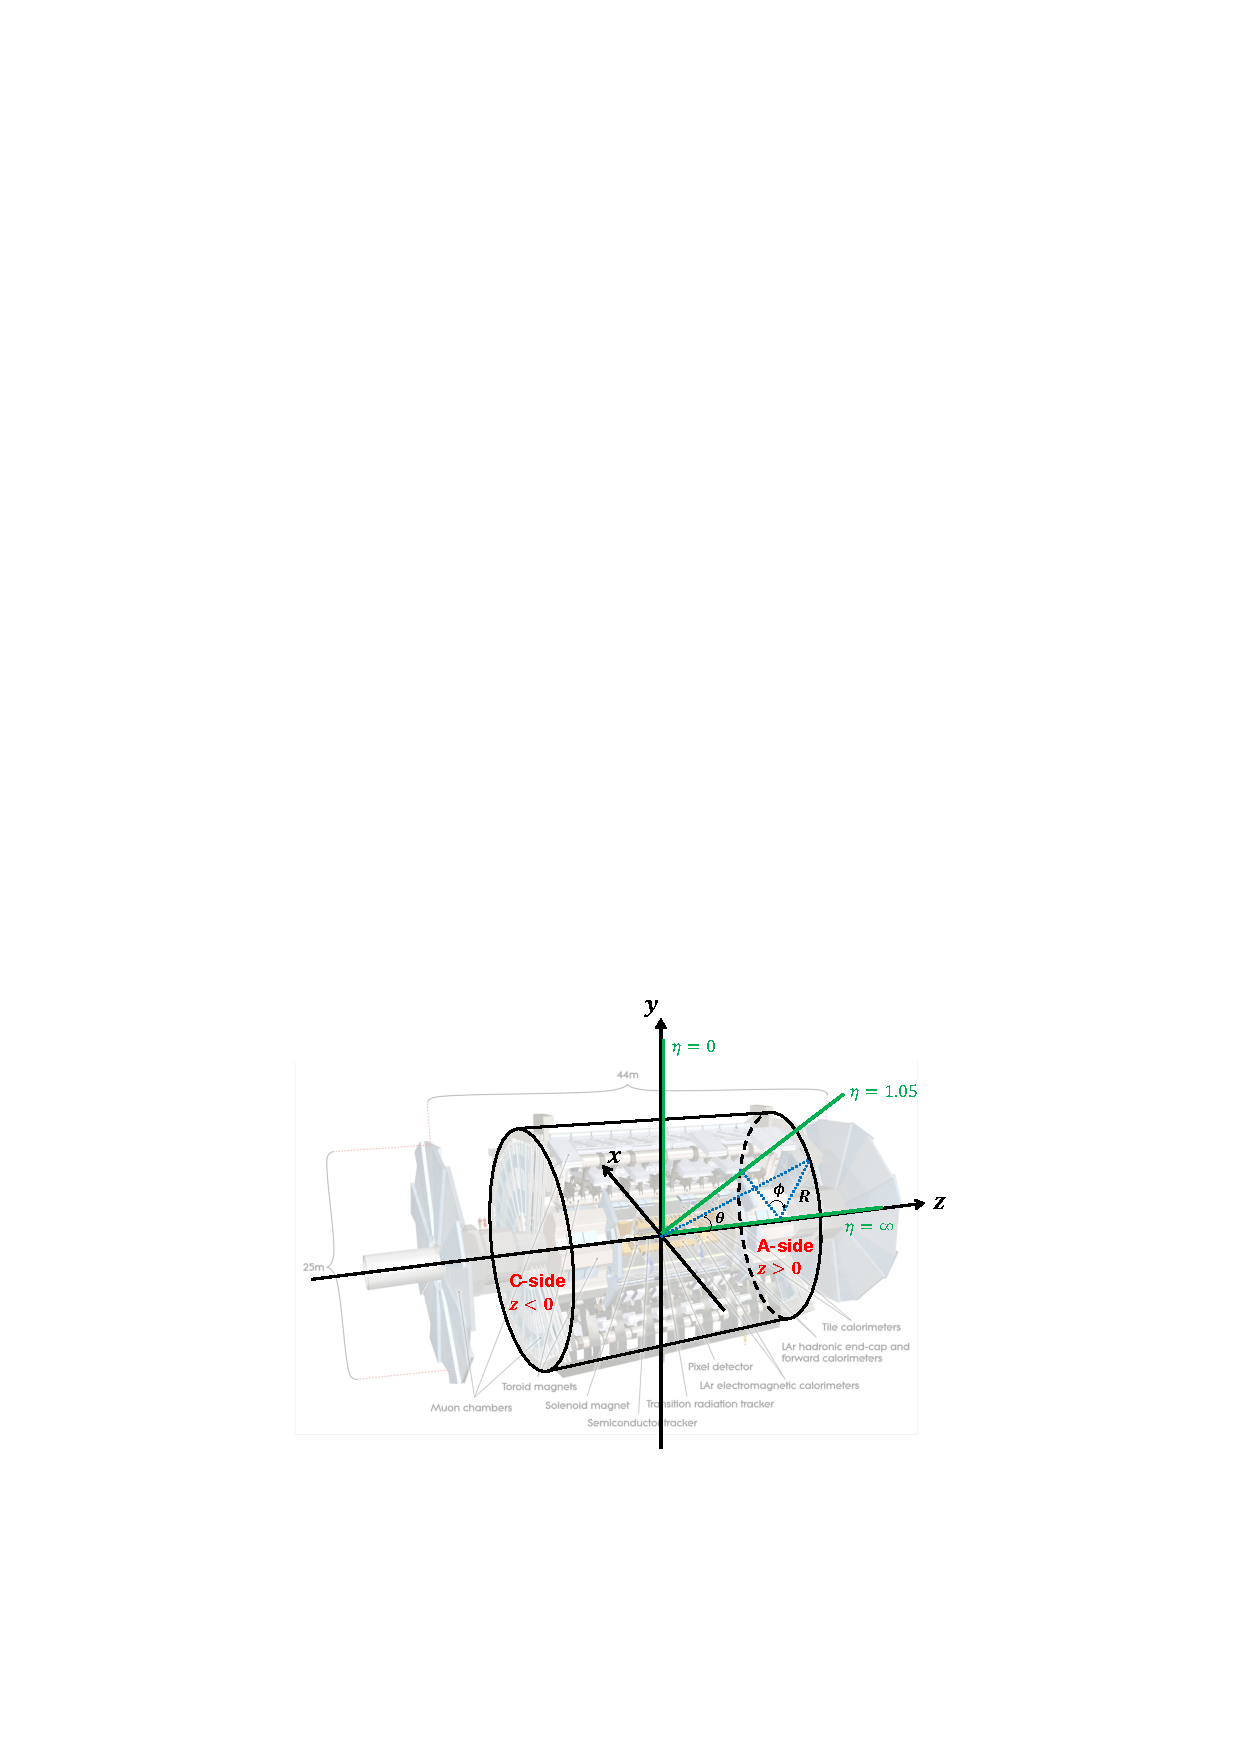
\includegraphics[width=16cm]{fig/Intro/ATLAScordination.pdf}
    \caption[ATLAS検出器における座標系]{ATLAS検出器で用いられる座標系。ビーム軸方向をz軸、LHC中心方向をx軸正の向きとした右手系で定義される。$z>0$をA side、$z<0$をC sideと呼ぶ。円筒座標系も利用され、特に検出器を覆う領域を説明するのに$\eta$が利用される。}
    \label{ATLAScordination}
    \end{figure}
  
    \subsection{ATLAS検出器における超伝導磁石}
    ATLAS検出器では荷電粒子の運動量を測定するため2種類の超伝導磁石が設置されている。図\ref{ATLASmagnet}にATLAS検出器における超伝導磁石の配置を示す。ソレノイド磁石は内部飛跡検出器とカロリメーターの間の領域に設置され、内部飛跡検出器内で荷電粒子を曲げるのに利用される。トロイド磁石はカロリメーターの外側に設置され、内部検出器を透過してきたミューオンを曲げるのに利用される。バレル部とエンドキャップ部のトロイド磁石は互いの干渉を避けるため22.5度ずらして設置されるが、双方の磁場は干渉してしまうため、生成される磁場は$\eta$方向にも$\phi$方向にも均一ではない。そのためミューオンの運動量は飛跡の曲率から直接逆算することが難しく、直線飛跡との角度比較を元に行われる。その方法の詳細は\ref{subsec_trigger_concept}節で説明する。

    \begin{figure} 
        \centering
        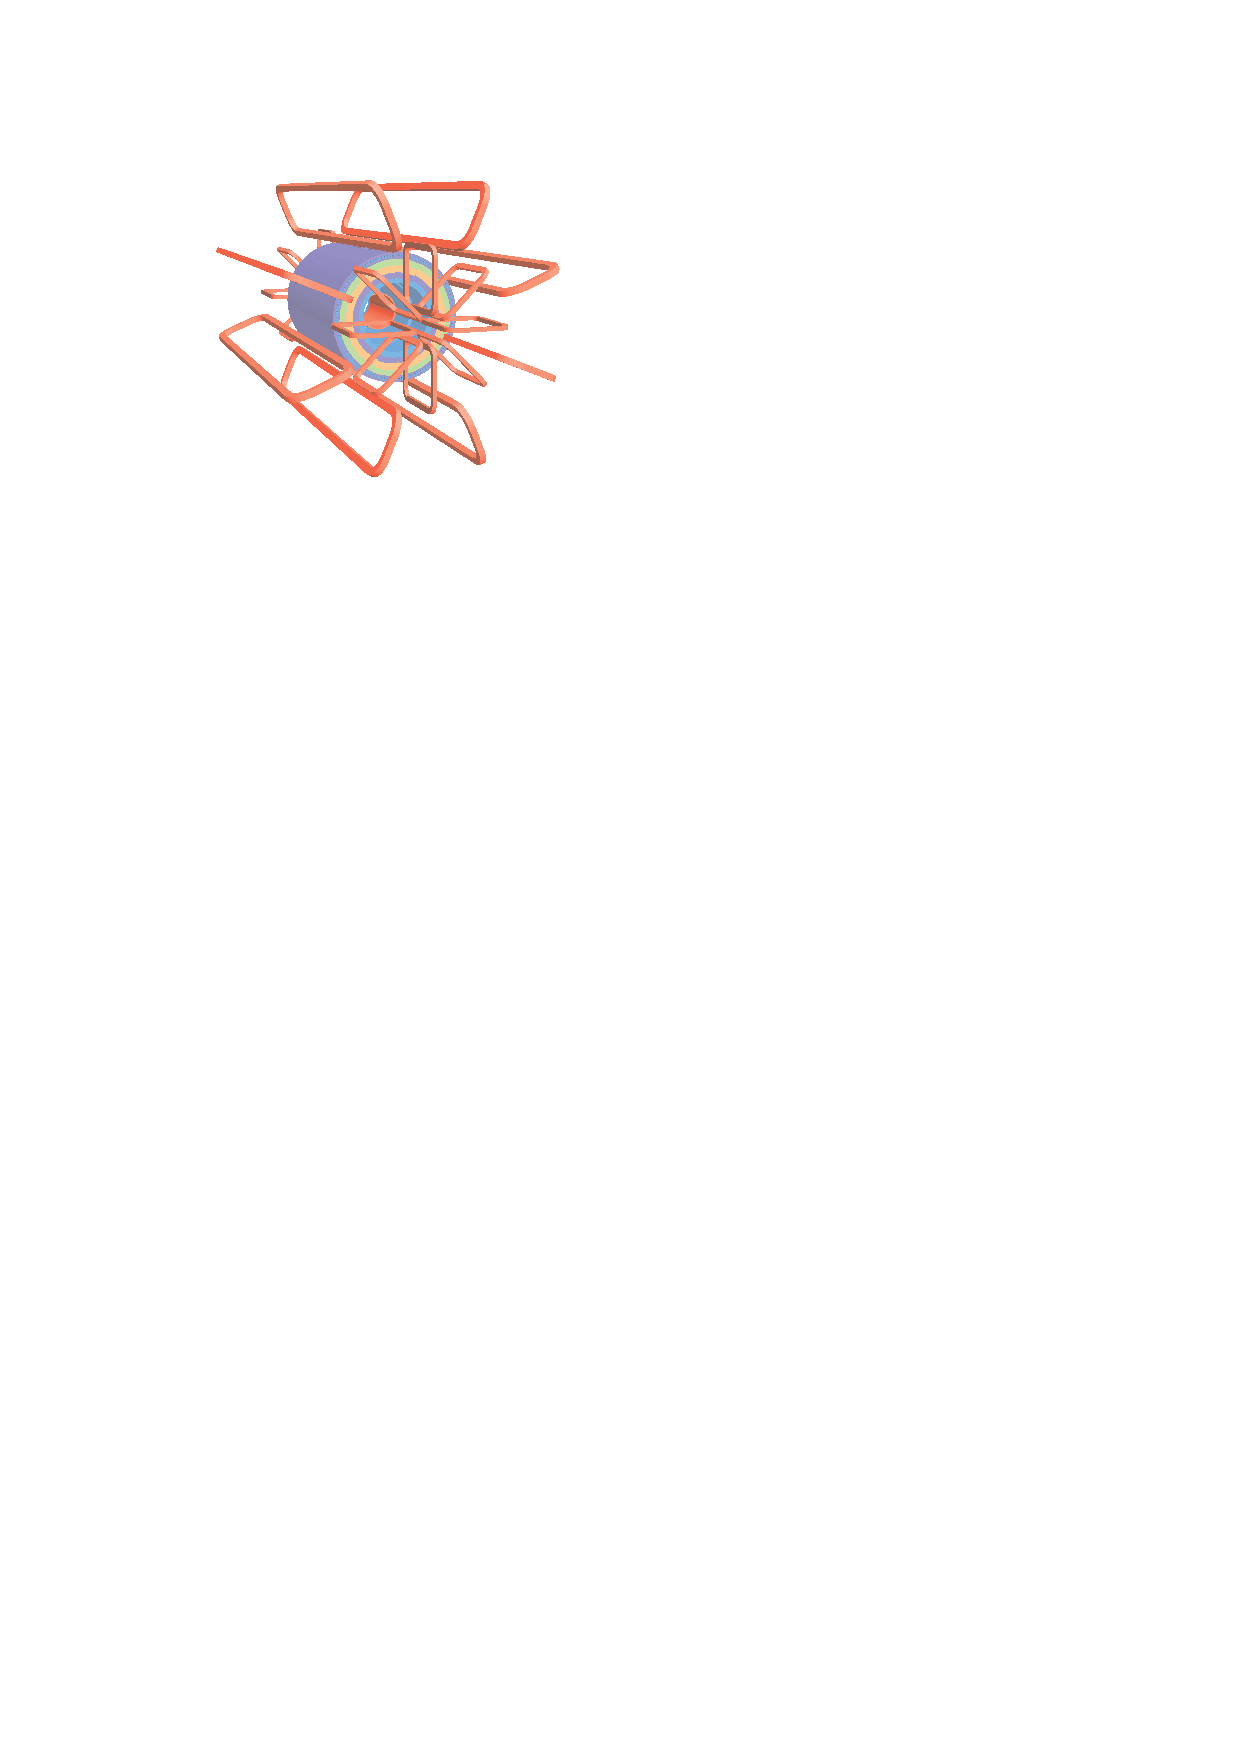
\includegraphics[width=16cm]{fig/Intro/ATLASmagnet.pdf}
        \caption[超伝導磁石の配置]{超伝導磁石の配置\cite{JINST:2008}。内部飛跡検出器を囲うようにソレノイド磁石が、カロリメーターの外側にトロイド磁石が設置されている。トロイド磁石はバレル部とエンドキャップ部で干渉の内容22.5度ずらして設置される。}
        \label{ATLASmagnet}
    \end{figure}
  
    \subsection{ミューオンスペクトロメーター}
    \label{subsec_Muonspectrometer}
本節ではATLAS検出器の中で、本研究に関係するミューオンスペクトロメーターについて述べる。ミューオンスペクトロメーターはATLAS検出器最外層に設置された検出器で、カロリーメーターを透過したミューオンの横方向運動量を測定する役割を担う。ミューオンスペクトロメーターは主にMonitored Drift Tube  (MDT) 、Resistive Plate Chamber  (RPC) 、Thin Gap Chamber  (TGC)  検出器で構成される。RPCとTGCは時間分解能に優れ、応答時間も高速であるためトリガーに利用される。MDTは位置分解能に優れているため、運動量の精密測定に利用される。トロイド磁場内部にはトリガー用の検出器としてTile Calorimeter、TGC EI、RPC BIS78、NSW、が設置されている。

各検出器の設置される領域を図\ref{Muonspectrometer2}に示す。ミューオンスペクトロメーターはトロイドマグネットの磁場構造に合わせて8回対称になっており、マグネットや支持構造と干渉しないよう、$\phi$方向にLarge sector、Small sectorという2種類のsectorに分かれている。トリガー用の検出器として|$\eta$| < 1.05のバレル領域ではRPC、1.05 < |$\eta$| < 2.4のエンドキャップ領域ではTGCが最外層に設置される。エンドキャップ領域において磁場内部の検出器がカバーする$\eta$、$\phi$領域を図\ref{SL_InnerCoin_covarage}に示す。1.3 < $\eta$ < 2.4の領域はNSWが網羅的にカバーしており、1.05 < $\eta$ < 1.3領域ではTGC EI、RPC BIS78、Tile カロリメーターがそれぞれ相補的にカバーしている。

\begin{figure} 
    \centering
    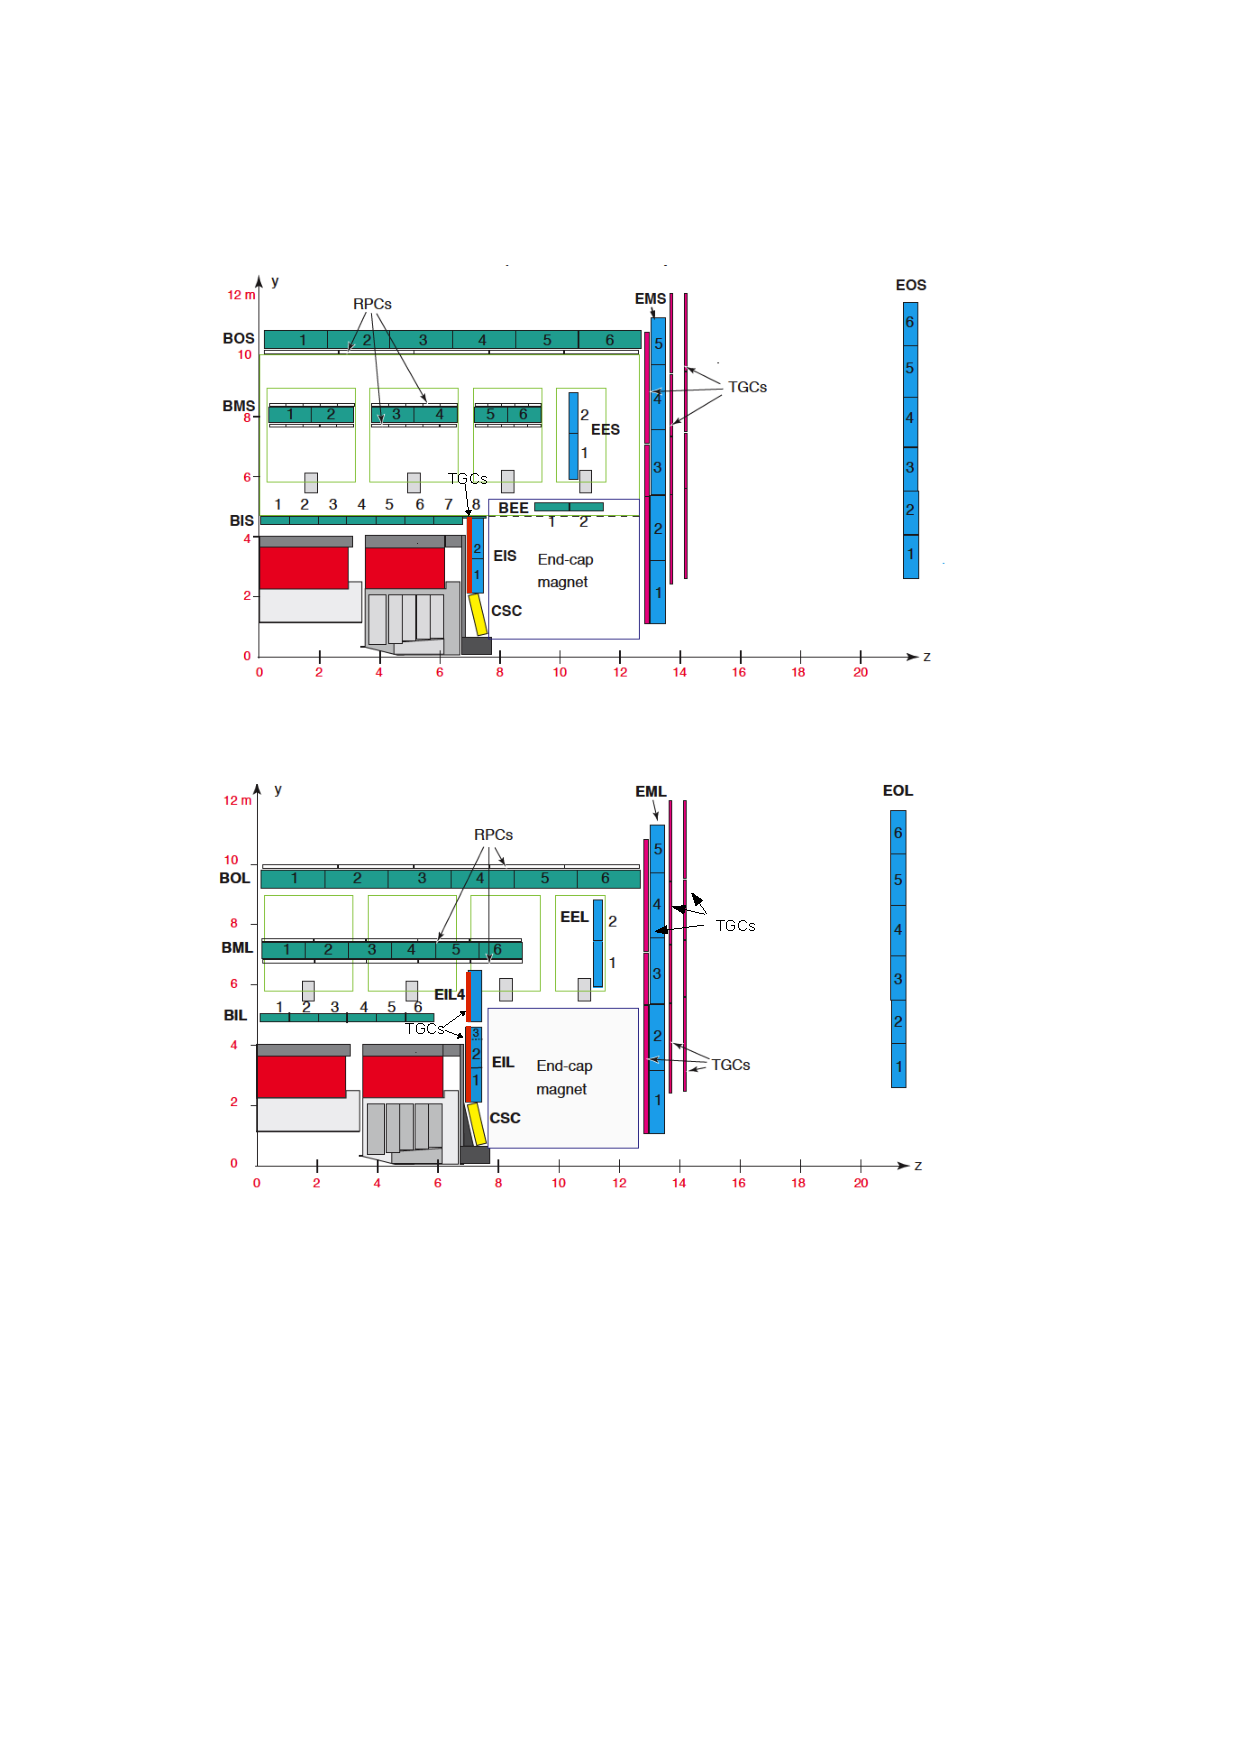
\includegraphics[width=16cm]{fig/Intro/Muonspectrometer.pdf}
    \caption[高輝度LHC-ATLAS実験でのミューオンスペクトロメーターの断面図]{高輝度LHC-ATLAS実験でのミューオンスペクトロメーターの断面図.\cite{tdr_phase2muon_2017017}
    }
    \label{Muonspectrometer2}
\end{figure}

\begin{figure} 
\centering
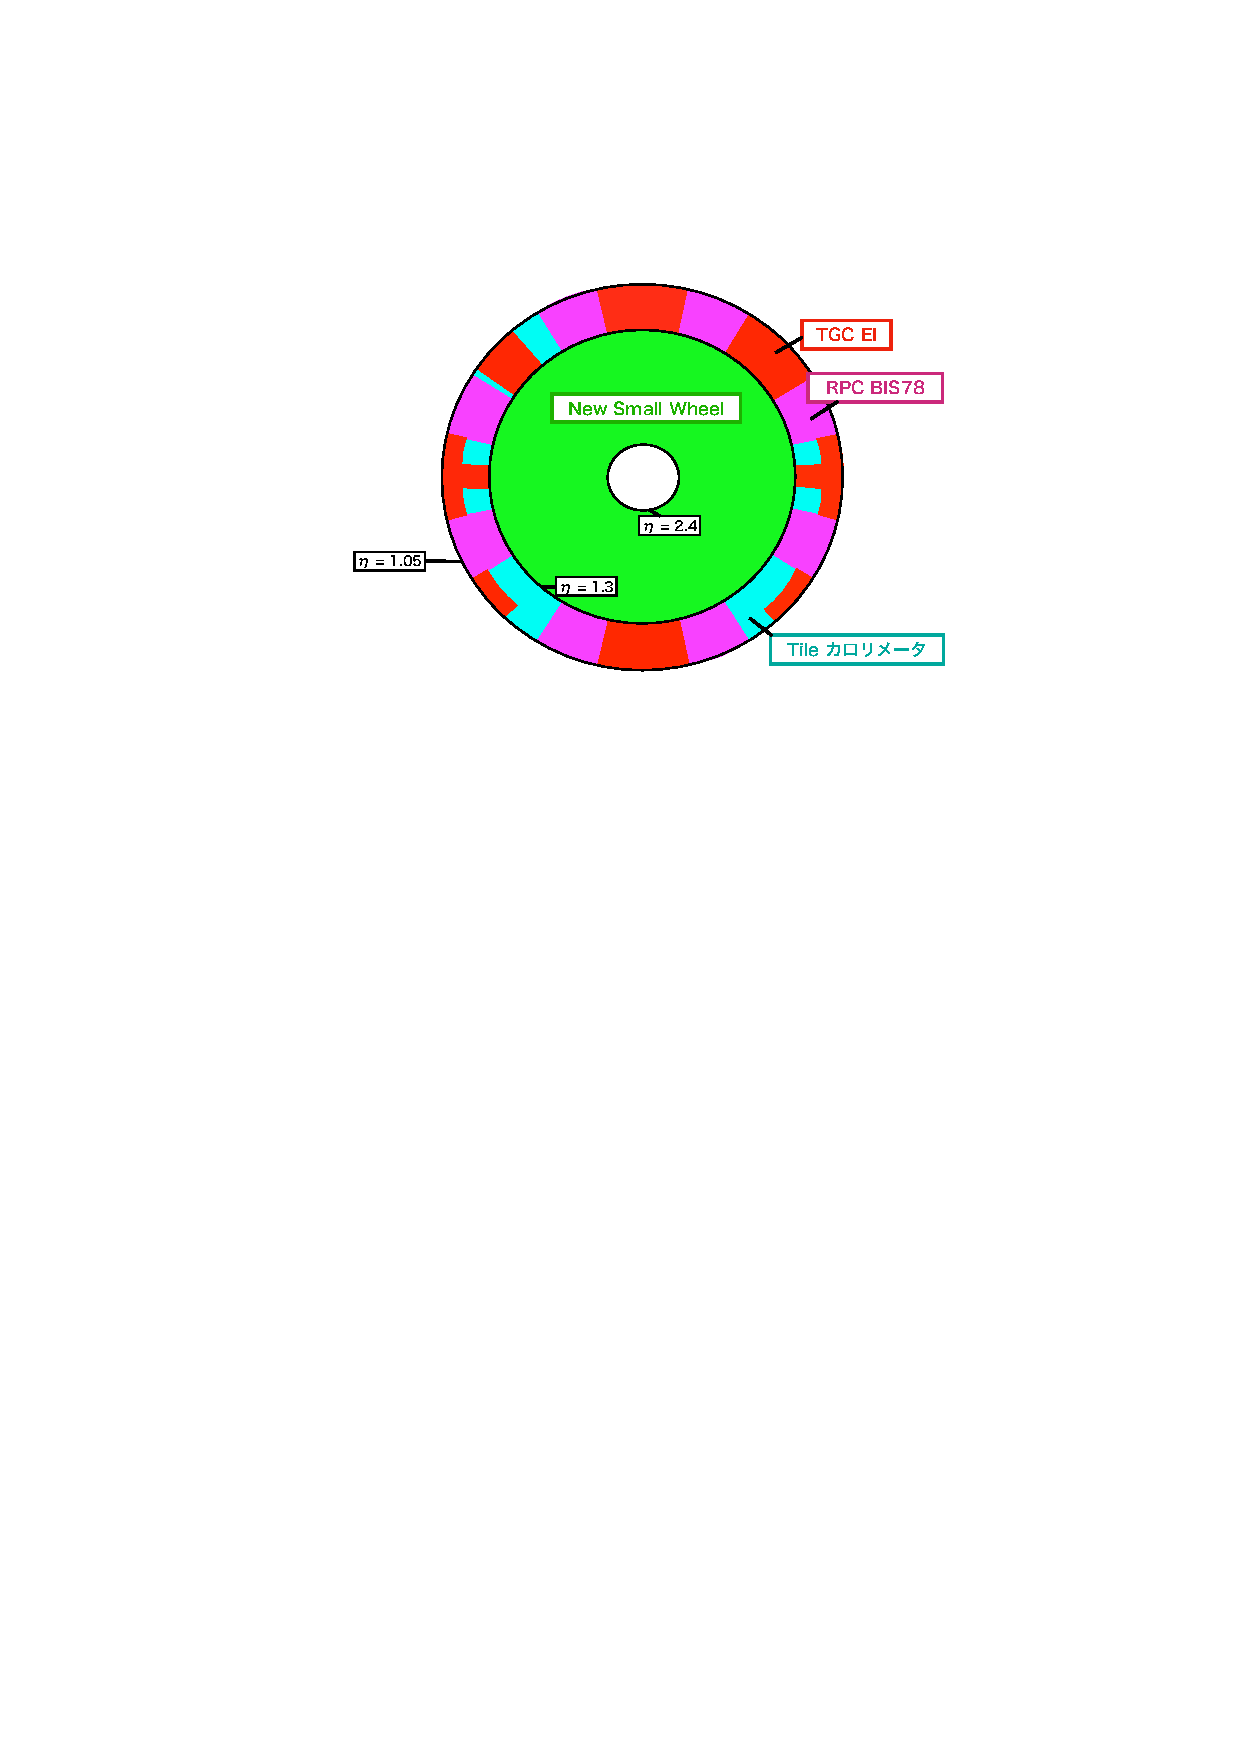
\includegraphics[width=16cm]{fig/Intro/SL_InnerCoin_covarage.pdf}
\caption[磁場内部の検出器でカバーされる$\eta$、$\phi$領域]{C磁場内部の検出器でカバーされる$\eta$、$\phi$領域\cite{mt_mino}}
\label{SL_InnerCoin_covarage}
\end{figure}


%TGC検出器
Thin Gap Chamber  (TGC) は1.05 < |$\eta$| < 2.4のエンドキャップ領域をカバーする円盤型のミューオントリガー検出器である。TGCはEndcapトロイドマグネットより内側に位置するEndcap Innner  (EI) と外側に位置するBig Wheel  (BW) に大別される。図\ref{TGC_picture}にBWの写真を示す。TGC BWはz方向に3つのステーションが連なって構成され、衝突点に近い方からM1、M2、M3ステーションと呼ぶ。各ステーションは2層または3層のガス層で構成されており、2層のものをdoublet、3層のものをtripletと呼ぶ。BWではM1がtriplet、M2、M3がdoubletになっている。

\begin{figure} 
\centering
\includegraphics[width=16cm]{fig/Intro/TGC_picture.jpg}
\caption[TGC検出器]{TGC検出器の正面写真 (M1)\cite{cern_document_server}}
\label{TGC_picture}
\end{figure}

TGCチェンバーの構造を図\ref{TGC_structure}に示す。TGCはアノードワイヤー間隔が1.8mm、アノードとカソードストリップの間隔が1.4 mmであるMWPCである。ワイヤーはR方向、ストリップは$\phi$方向に直交して張られており、2次元位置を読み出すことができる。ガス層には$CO_2/nC_5H_{12}$が55:45で混合されたガスが充填されている。

\begin{figure}
\begin{minipage}[b]{.5\linewidth}
\centering
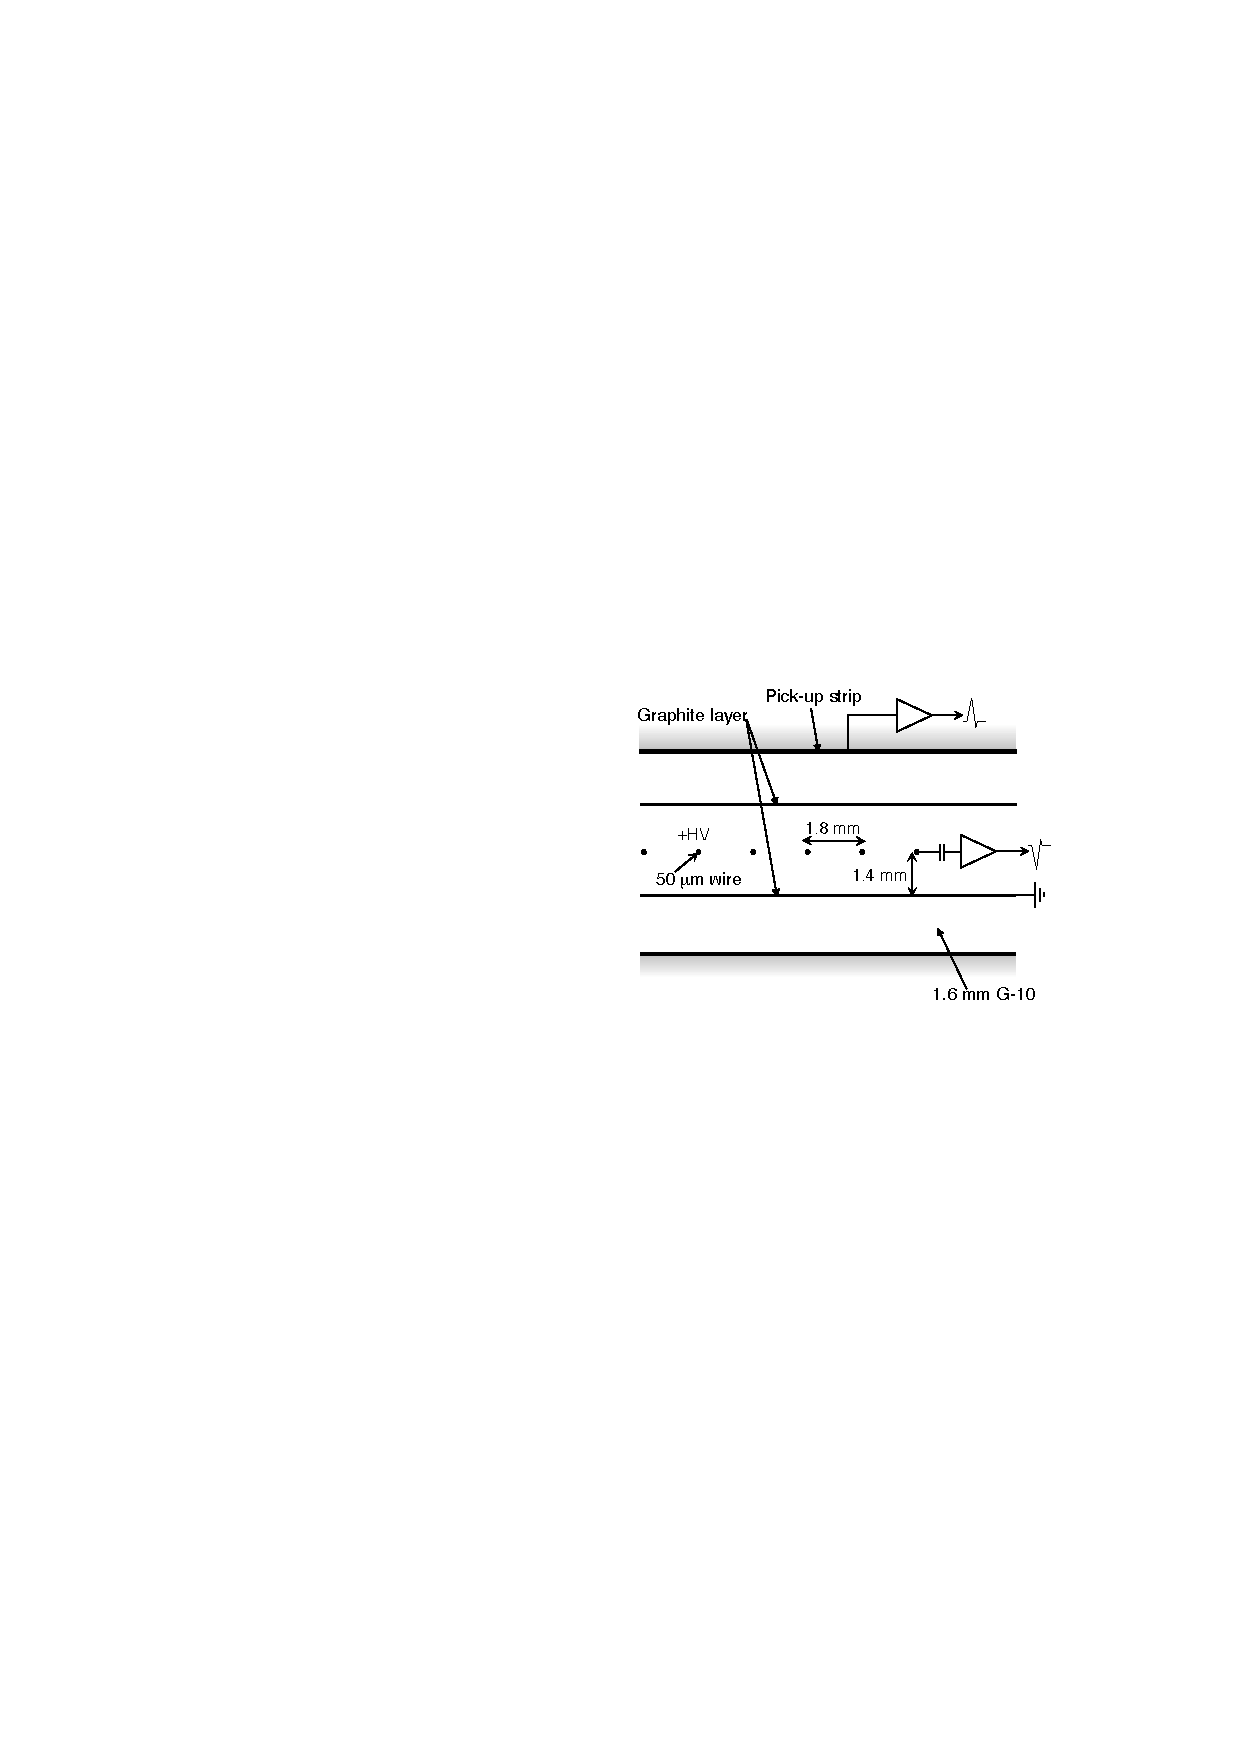
\includegraphics[height=5cm]{fig/Intro/TGC_structure.pdf}
\subcaption{TGCチェンバーの断面図}
\end{minipage}%
\begin{minipage}[b]{.5\linewidth}
\centering
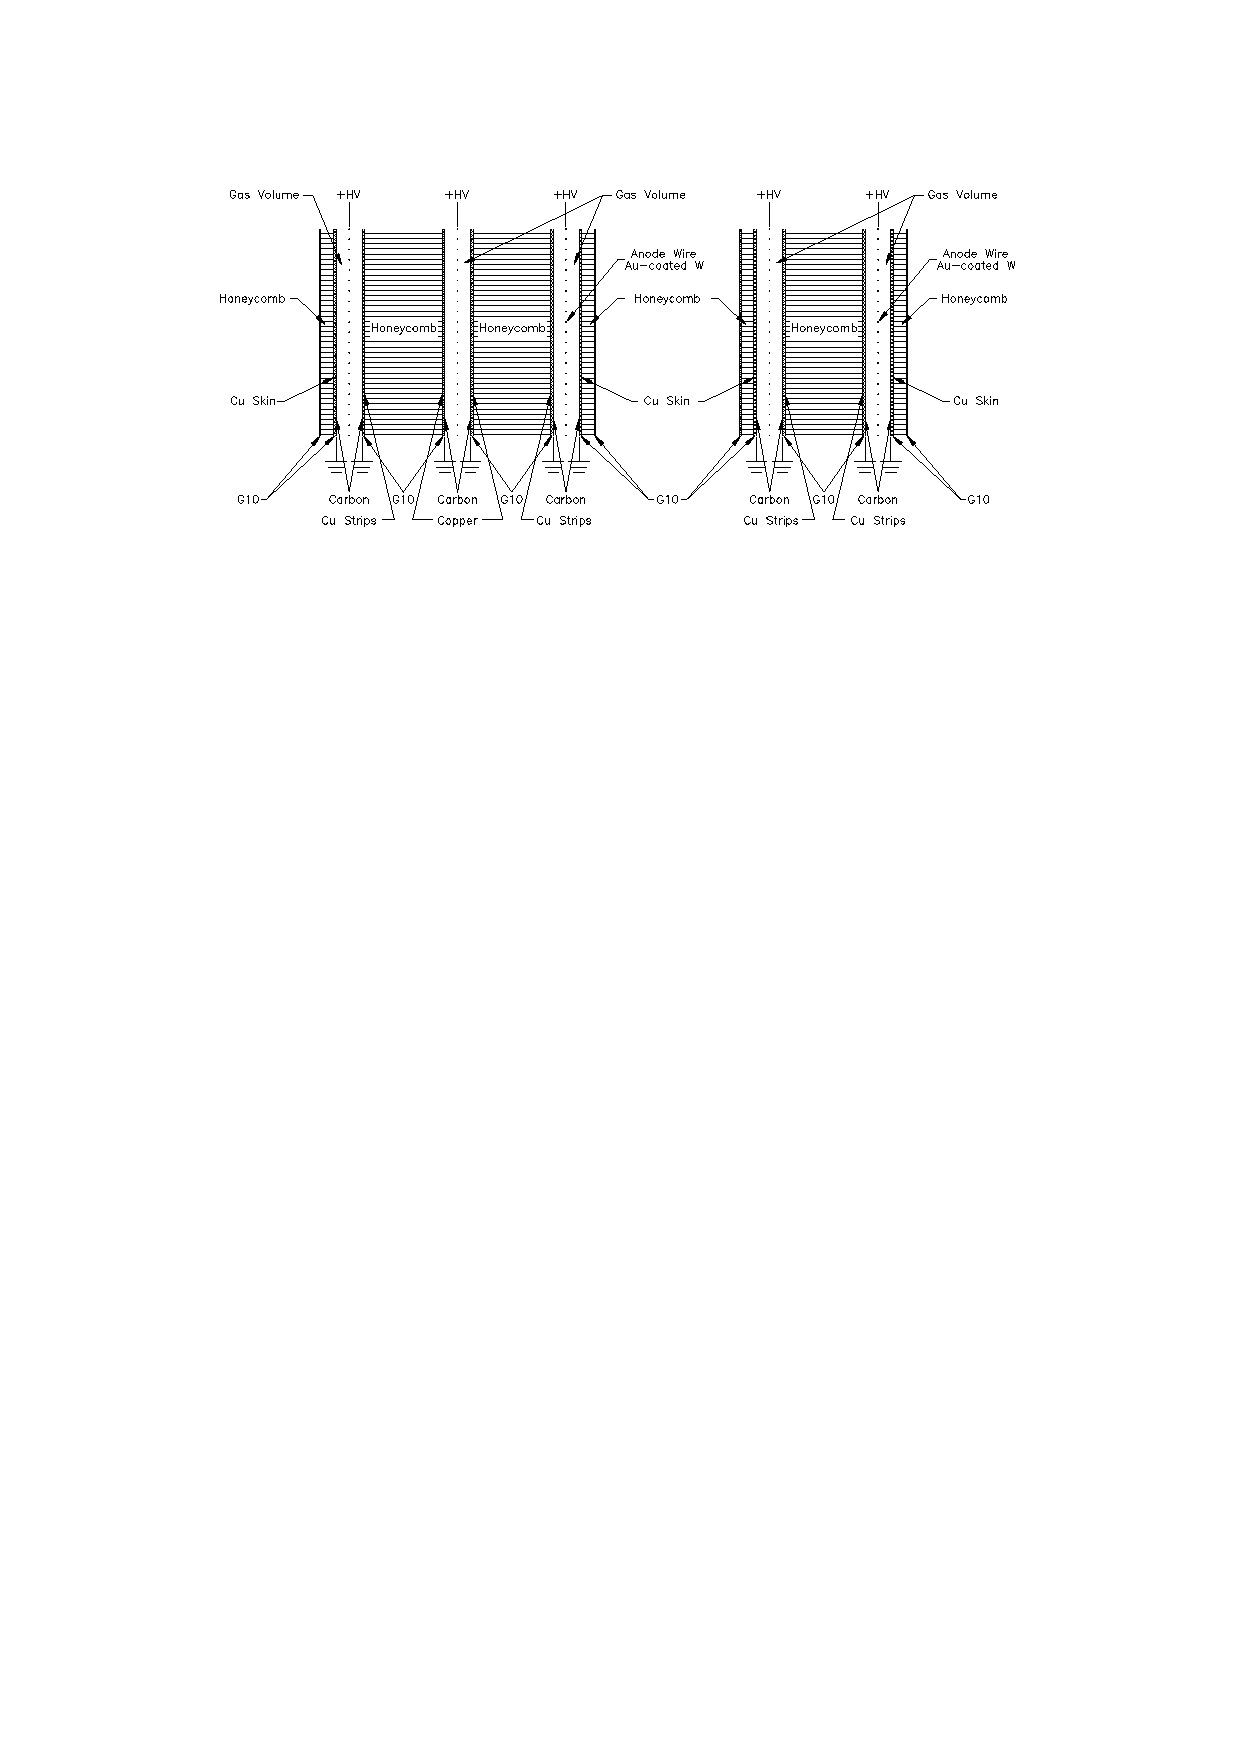
\includegraphics[height=5cm]{fig/Intro/TGC_crosssection.pdf}
\subcaption{TGC doubletとtripletの断面図}
\end{minipage}%
\caption[TGCチェンバーの断面図]{ (a)はTGCチェンバーの断面図を表す\cite{JINST:2008}。ワイヤーとストリップが直交して張られていることがわかる。 (b)はTGC doubletとtripletの断面図である。それぞれ2層、3層のガスギャップで構成されており、各ガスギャップの間はペーパーハニカムにより満たされている。}
\label{TGC_structure}
\end{figure}


荷電粒子がTGCに入射すると、電磁相互作用によりガス分子が電離される。電離した電子はワイヤーに印加された2.8 kVの電圧によりワイヤー方向に集められ、ワイヤー付近に到達すると強い電場により電子雪崩を生じる。ワイヤーでは電子雪崩で生じた正イオンのドリフトが、ストリップではそれらの鏡像電荷が電流信号として検出される。

TGC検出器はトリガー用の検出器であり、ガスギャップが薄く、ワイヤー間隔が小さいため時間応答がよい。これにより陽子衝突頻度である25 nsより細かな時間分解能でミューオンを検出し、そのミューオンがどの陽子バンチ衝突に由来するのかを識別 ( Bunch Crossing IDentification, BCID) することができる。一方、TGC検出器はそれほど高い位置分解能が求められていないため、ワイヤー電極を4 $\sim$ 20本まとめてから読み出しを行う。結果としてワイヤー、ストリップは合計32万チャンネルをもつ。

BWの外側  (1.05 < |$\eta$| < 1.92) はエンドキャップ領域、円盤の内側  (1.92 < |$\eta$|< 2.4) はフォワード領域と呼ばれる。エンドキャップ領域では$\phi$方向に48回対称になるよう、フォワードでは$\phi$方向に24回対称になるようにチェンバーが設置されている。エンドキャップ領域の1/48、フォワードの1/24はトリガー回路的に独立しており、それぞれが"トリガーセクター"と呼ばれる。
また電源供給、ガス供給、電気回路制御、読み出しの観点からBWは$\phi$方向に12個のセクターに分割される。各"1/12セクター"はx軸の正の方からy軸の正の方向に向かって順にA-sideではA01からA12、C-sideではC01からC12までの名前がついている。

\section{ATLAS実験におけるTDAQシステム}
\label{sec_TDAQ}
   
    \subsection{Run3でのTDAQシステム}
    \label{subsec_run3TDAQ}
    LHCでは25 nsの間隔で陽子バンチが衝突するため、衝突で生じたすべてのデータを保存することはできない。限られた読み出し帯域とオフラインの計算リソースを最大限有効活用するためには興味のある衝突事象のみを記録するトリガーが重要となる。またトリガー判定がなされたイベントに対して正しくデータを取得するには、トリガーシステムとデータ取得 (data acquisition、DAQ) システムが連動して機能する必要がある。ATLAS実験では、トリガーとデータ取得をまとめてTrigger and Data Acquisition (TDAQ) システムと呼ぶ。図\ref{Run3_TDAQ}にRun3におけるTDAQシステムの概要を示す。ATLASのトリガーシステムはLevel-1という初段のハードウェアトリガーと、それに続くHigh Level Trigger (HLT) という後段のソフトウェアトリガーから構成される。

    \begin{figure} 
    \centering
    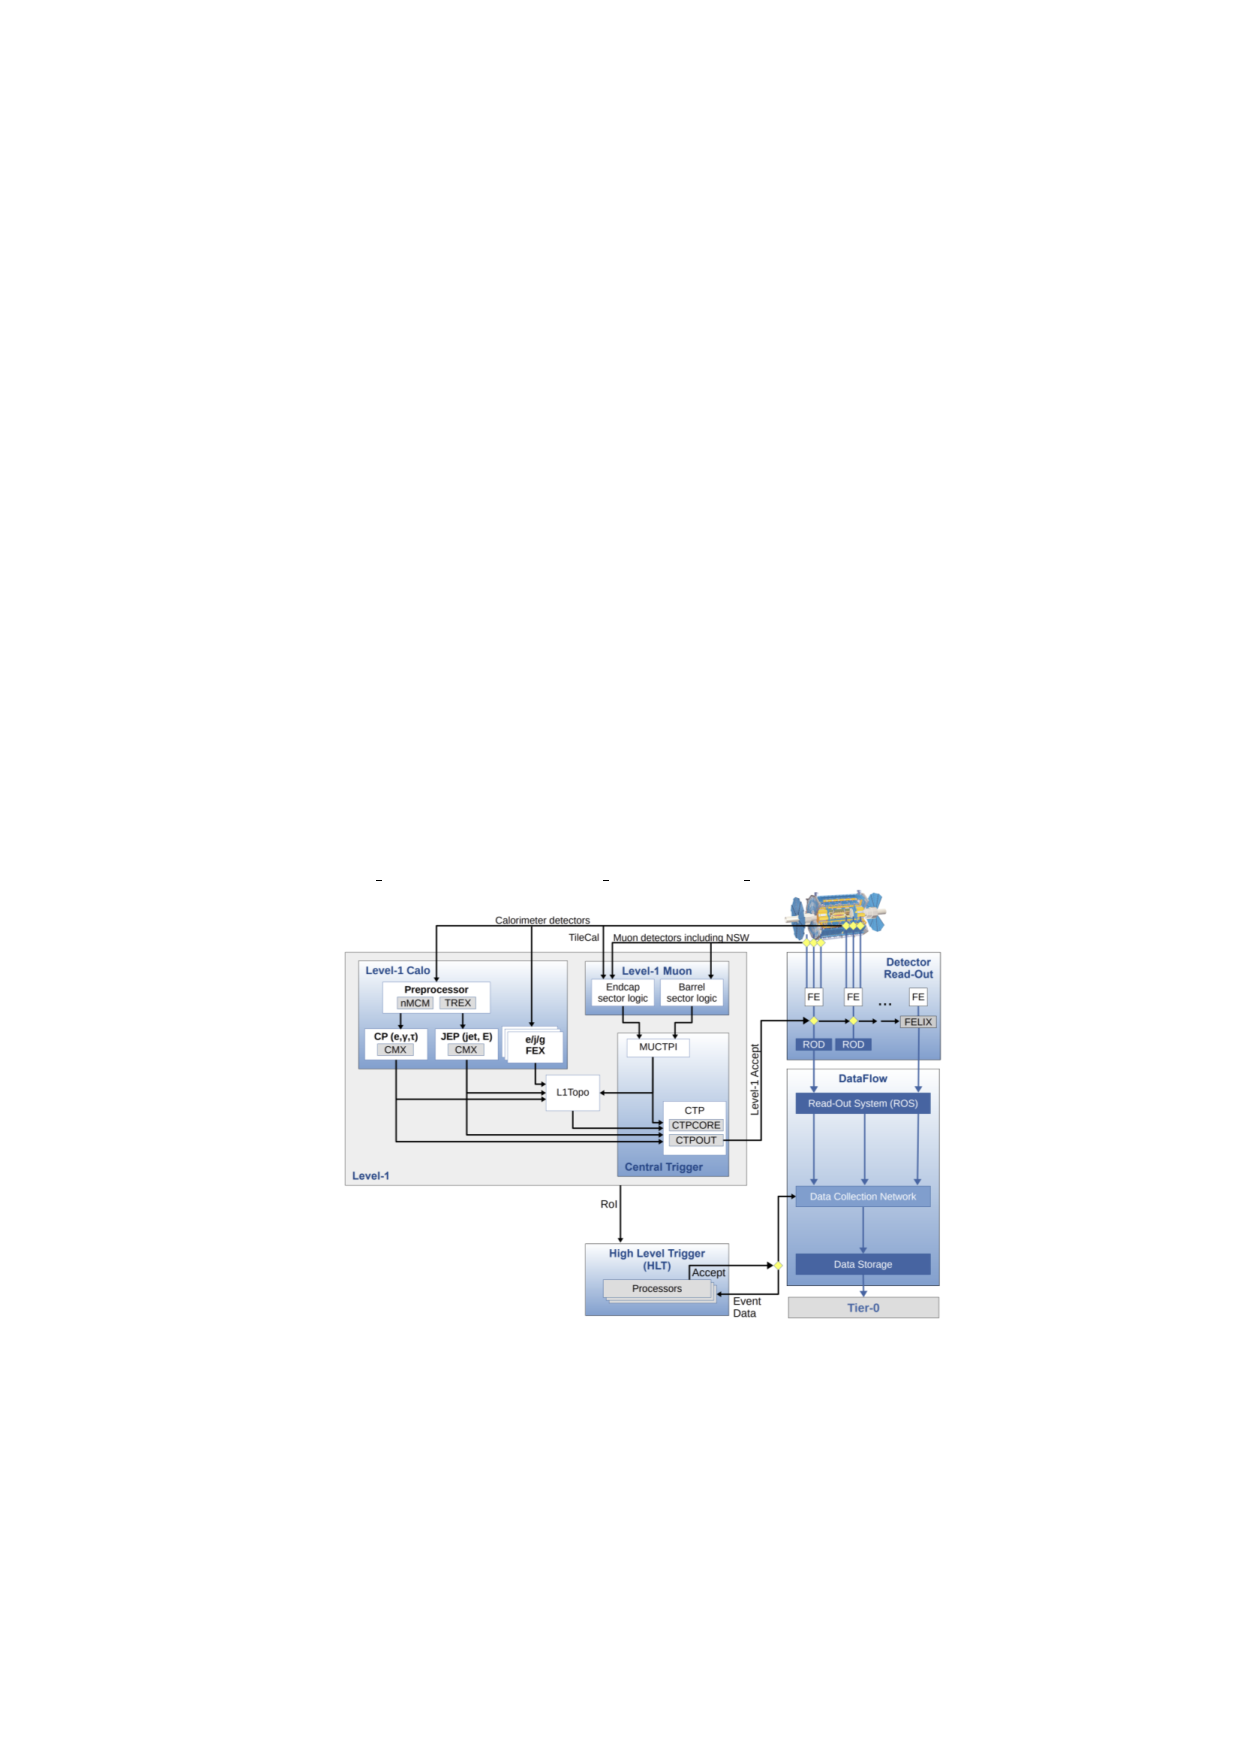
\includegraphics[width=16cm]{fig/Intro/Run3_TDAQ.pdf}
    \caption[Run3におけるTDAQシステムの概要]{Run3におけるTDAQシステムの概要\cite{Run3_TDAQ}。トリガーシステムはLevel-1 Triggerという初段ハードウェアトリガーとHigh Level Trigger (HLT)という後段のソフトウェアトリガーから構成される。L1 TriggerはL1 CaloとL1 Muonに大別されCTPで総合的なトリガー判定がなされる。L1 TriggerをパスしたイベントはHLTでより精度の高いトリガー判定が行われ、CERN Permanent Strageに保存される。 }
    \label{Run3_TDAQ}
    \end{figure}

    \subsubsection{Level-1 Trigger}
    \vskip0.5\baselineskip
    Level-1 Triggerは25 ns間隔で行われるすべての陽子バンチ衝突事象の中から、物理的に興味のあるオブジェクトを含むイベントを大まかに選別する初段トリガーである。L1 Triggerによってイベントレートは40 MHzから100 kHzまで削減される。L1 Triggerは大量のデータを高速で処理する必要があるため、ASICやFPGAなどのハードウェアを利用したトリガー判定が行われる。
    ATLASでのL1 Triggerシステムは主にLevel-1 CaloとLevel-1 Muonで構成される。Level-1 Caloはカロリーメーターからのエネルギー情報をもとに発行されるトリガーで、高いエネルギーを持つ電子、光子、ジェットを含むイベントに対してトリガーが発行される。Level-1 Muonは主にRPCとTGCからの情報をもとに発行されるトリガーで、横方向運動量の大きなMuonを含むイベントに対してトリガーが発行される。これらの信号はCentral Trigger Processor (CTP) に渡され、総合的にLevel-1トリガー判定が行われる。L1 Triggerが発行されると各検出器のフロントエンド回路にはLevel-1 Accept (L1A) が送られ、そのバンチ衝突に由来する検出器のヒット信号がReadout Driver (ROD) へと送られる。
    Level-1 Triggerではバンチ衝突が生じてからL1Aが届けられるまでの時間 (Level-1 レイテンシー) が一定であるFIxed Latency Schemeを採用している。陽子バンチ衝突で生じるデータはL1Aが出されるまでの間、各フロントエンドエレクトロニクス上のバッファーに保管される。L1レイテンシーは設置可能なバッファーサイズによって制限されており、Run3では2.5 $\mu\mathrm{s}$に設定されている。

    \subsubsection*{High Level Trigger (HLT) }
    \vskip0.5\baselineskip
    HLTは初段トリガーをパスしたイベントから最終的にストレージに保存する事象を選ぶ役割を担う、ソフトウェアベースのトリガーである。初段トリガーでは使われなかった内部飛跡検出器やMDTなどの精密測定用検出器からの情報も利用して、より高い精度でイベント再構成を行う。HLTによりトリガーレートは1 kHzまで削減され、記録すべきと判断されたイベントは、永久保存のためにCERNのコンピューティングセンターであるTier-0へ送られる。

    \subsubsection*{トリガーメニュー}
    ATLAS実験は陽子陽子衝突で生じるさまざまな事象を取得することで、幅広い終状態を持つ多様な物理解析を展開する。そのためにも、広範な物理事象を取得できるよう、限られたトリガーレートを適切に分配する必要がある。そのために用意されているのが図\ref{Run2_Triggermenu}に示すようなトリガーメニューである。トリガーメニューでは、解析で利用されるlepton、jet、消失横方向エネルギー ($E_{\mathrm{T}^{\mathrm{miss}}}$)などの典型的なオブジェクトを取得するためのLevel-1およびHLTトリガーの閾値が定められる。このテーブルはトリガーレートのシミュレーションなどにより、全体を通して100 kHzおよび1 kHzのトリガーレートの制約を守るよう設計されている。

    \begin{figure} 
    \centering
    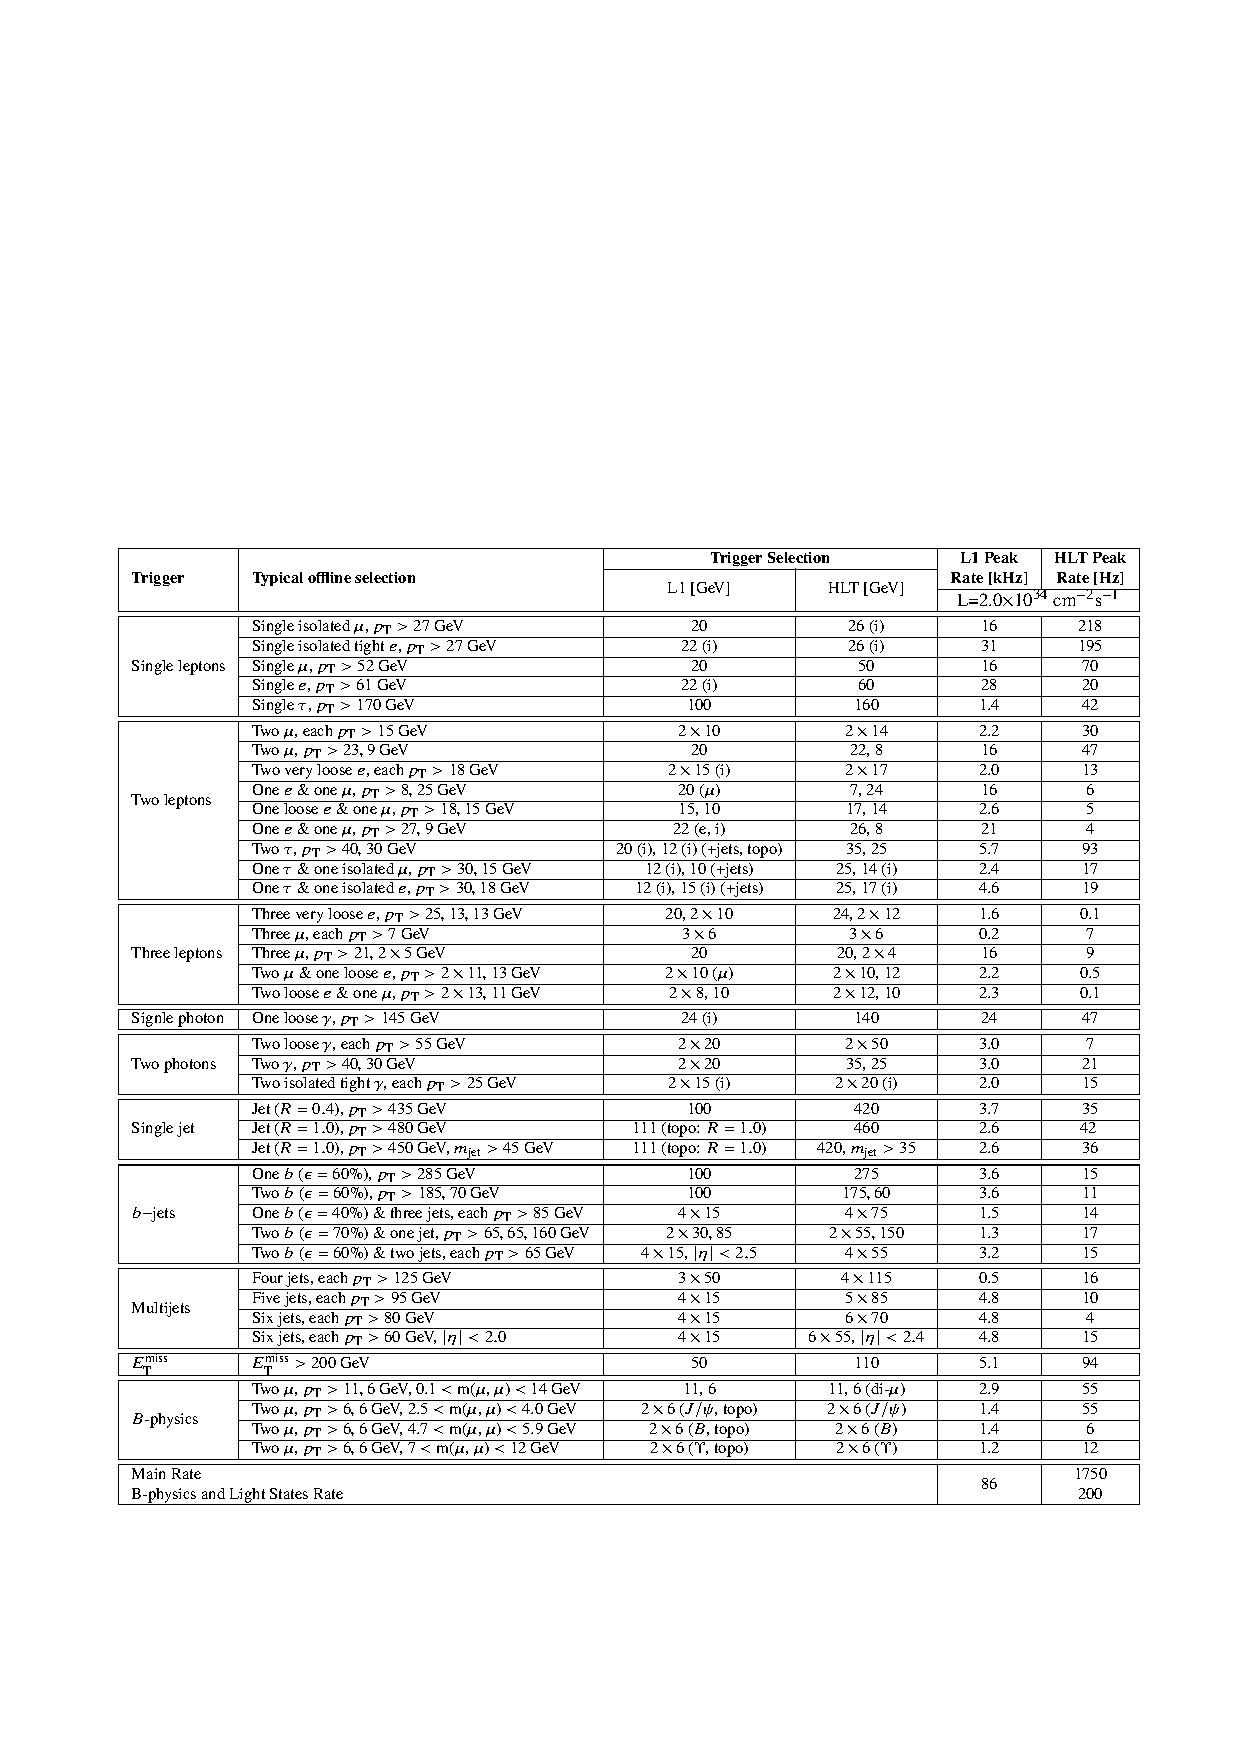
\includegraphics[width=16cm]{fig/Intro/Run2_Triggermenu.pdf}
    \caption[Run2でのトリガーメニューの一例]{Run2でのトリガーメニューの一例\cite{Run2_Triggermenu}。解析で利用される典型的なオブジェクトを取得するためのLevel-1およびHLTでのトリガー閾値が定められる。全体を通してトリガーレートの制約を守るよう設計される。}
    \label{Run2_Triggermenu}
    \end{figure}

    \subsection{高輝度LHC-ATLAS実験でのTDAQシステム}
2029年からビーム輝度を約3倍に増強した高輝度LHC実験が始まる。高輝度LHC実験ではパイルアップによる背景事象が大幅に増加し、結果としてトリガーレートが増加する。現行のTDAQシステムを維持しつつ読み出しレートの制約を守るためには、興味のある物理事象へのアクセプタンスを落とすことにつながる。そこで高輝度LHC実験に向けて大規模なTDAQシステムのアップグレードが行われる。初段トリガーレートは100 kHzから1 MHzへ、後段トリガーレートは1 kHzから10 kHzへと拡張される。さらに、初段トリガーレイテンシーも2.5 $\mu\mathrm{s}$から10 $\mu\mathrm{s}$へと拡張される。これにより洗練されたトリガーアルゴリズムを実装することができるようになる。図\ref{Phase2_TDAQ}に高輝度LHC実験でのTDAQシステムの概要を示す。
高輝度LHC実験では初段トリガーをLevel-0 Trigger、後段トリガーをEvent Filter (EF) と呼ぶ。

\begin{figure}
\begin{minipage}[b]{.5\linewidth}
\centering
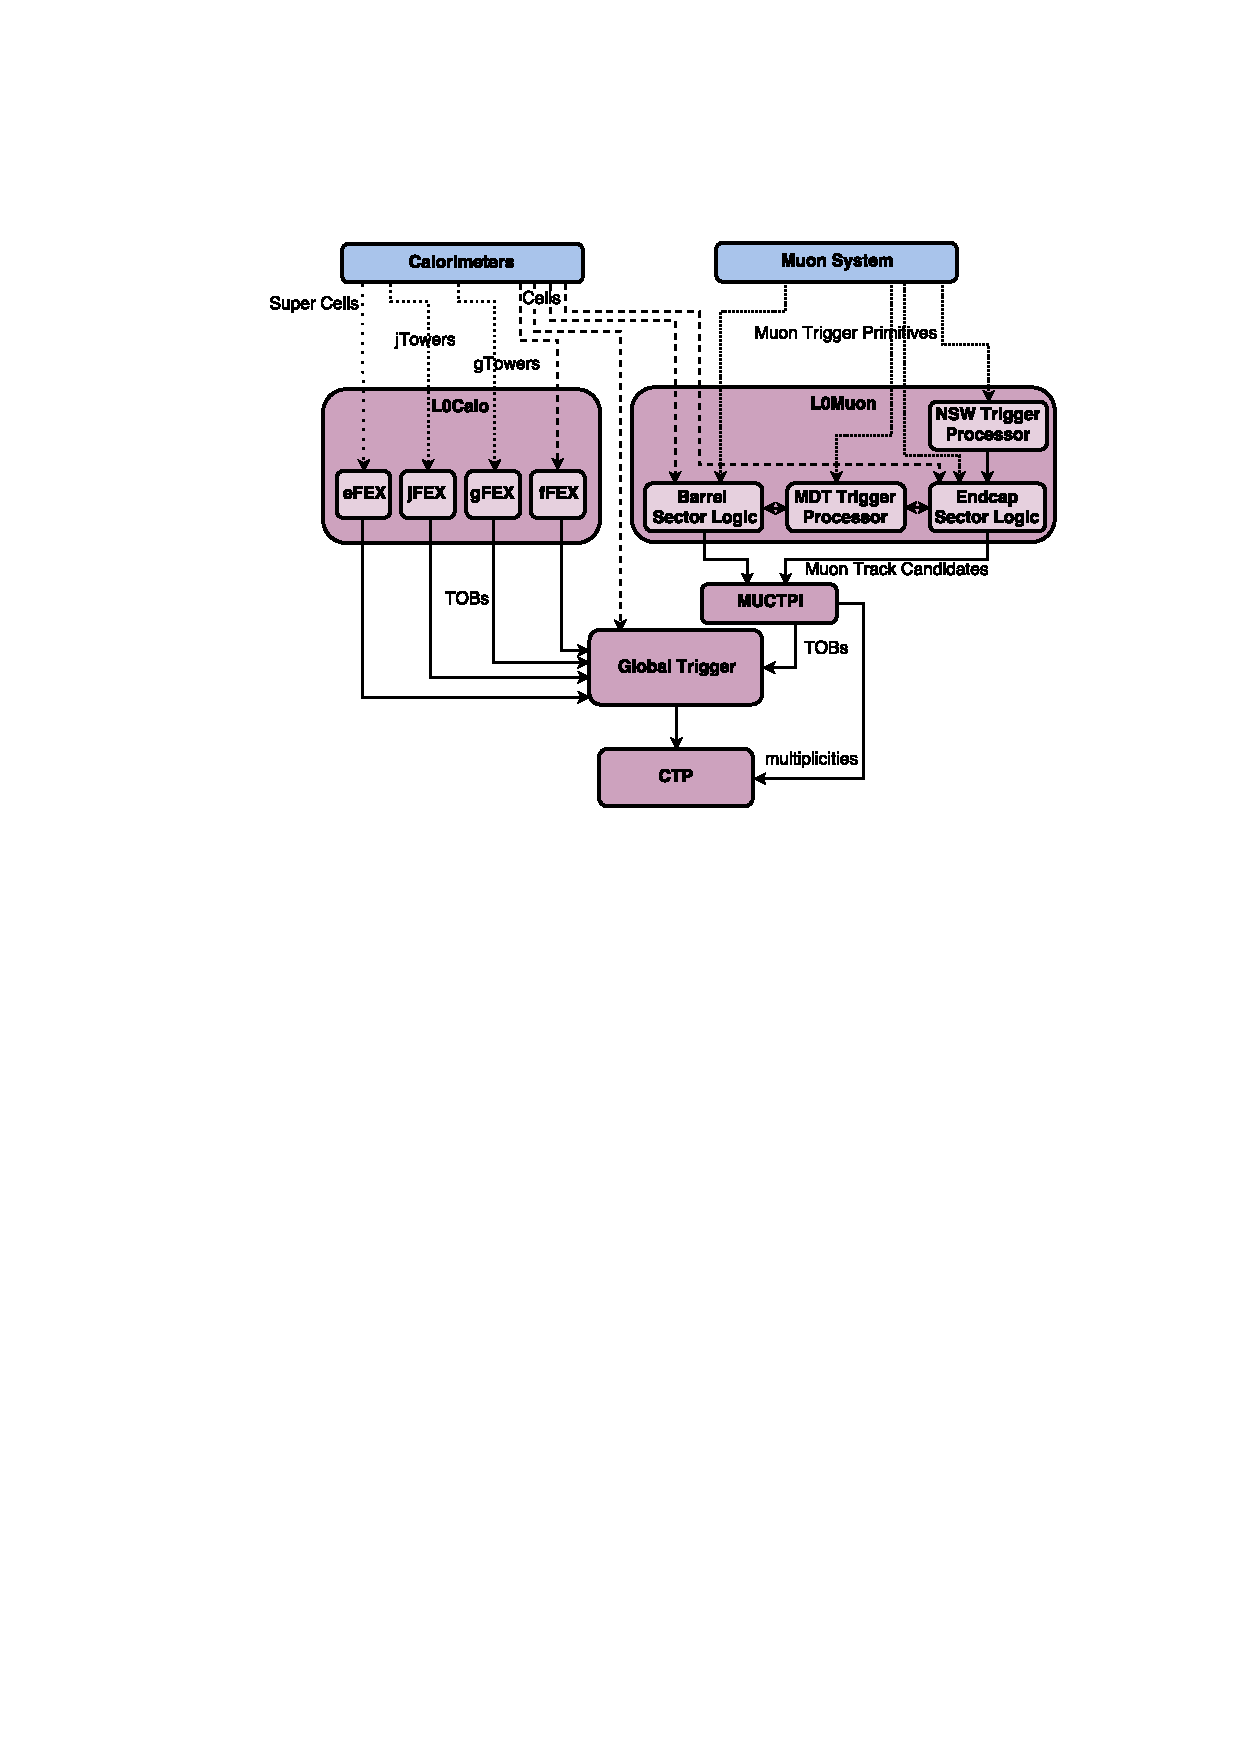
\includegraphics[height=7cm]{fig/Intro/Phase2_L0trigger.pdf}
\subcaption{Level-0 Triggerシステムの概要}
\end{minipage}%
\begin{minipage}[b]{.5\linewidth}
\centering
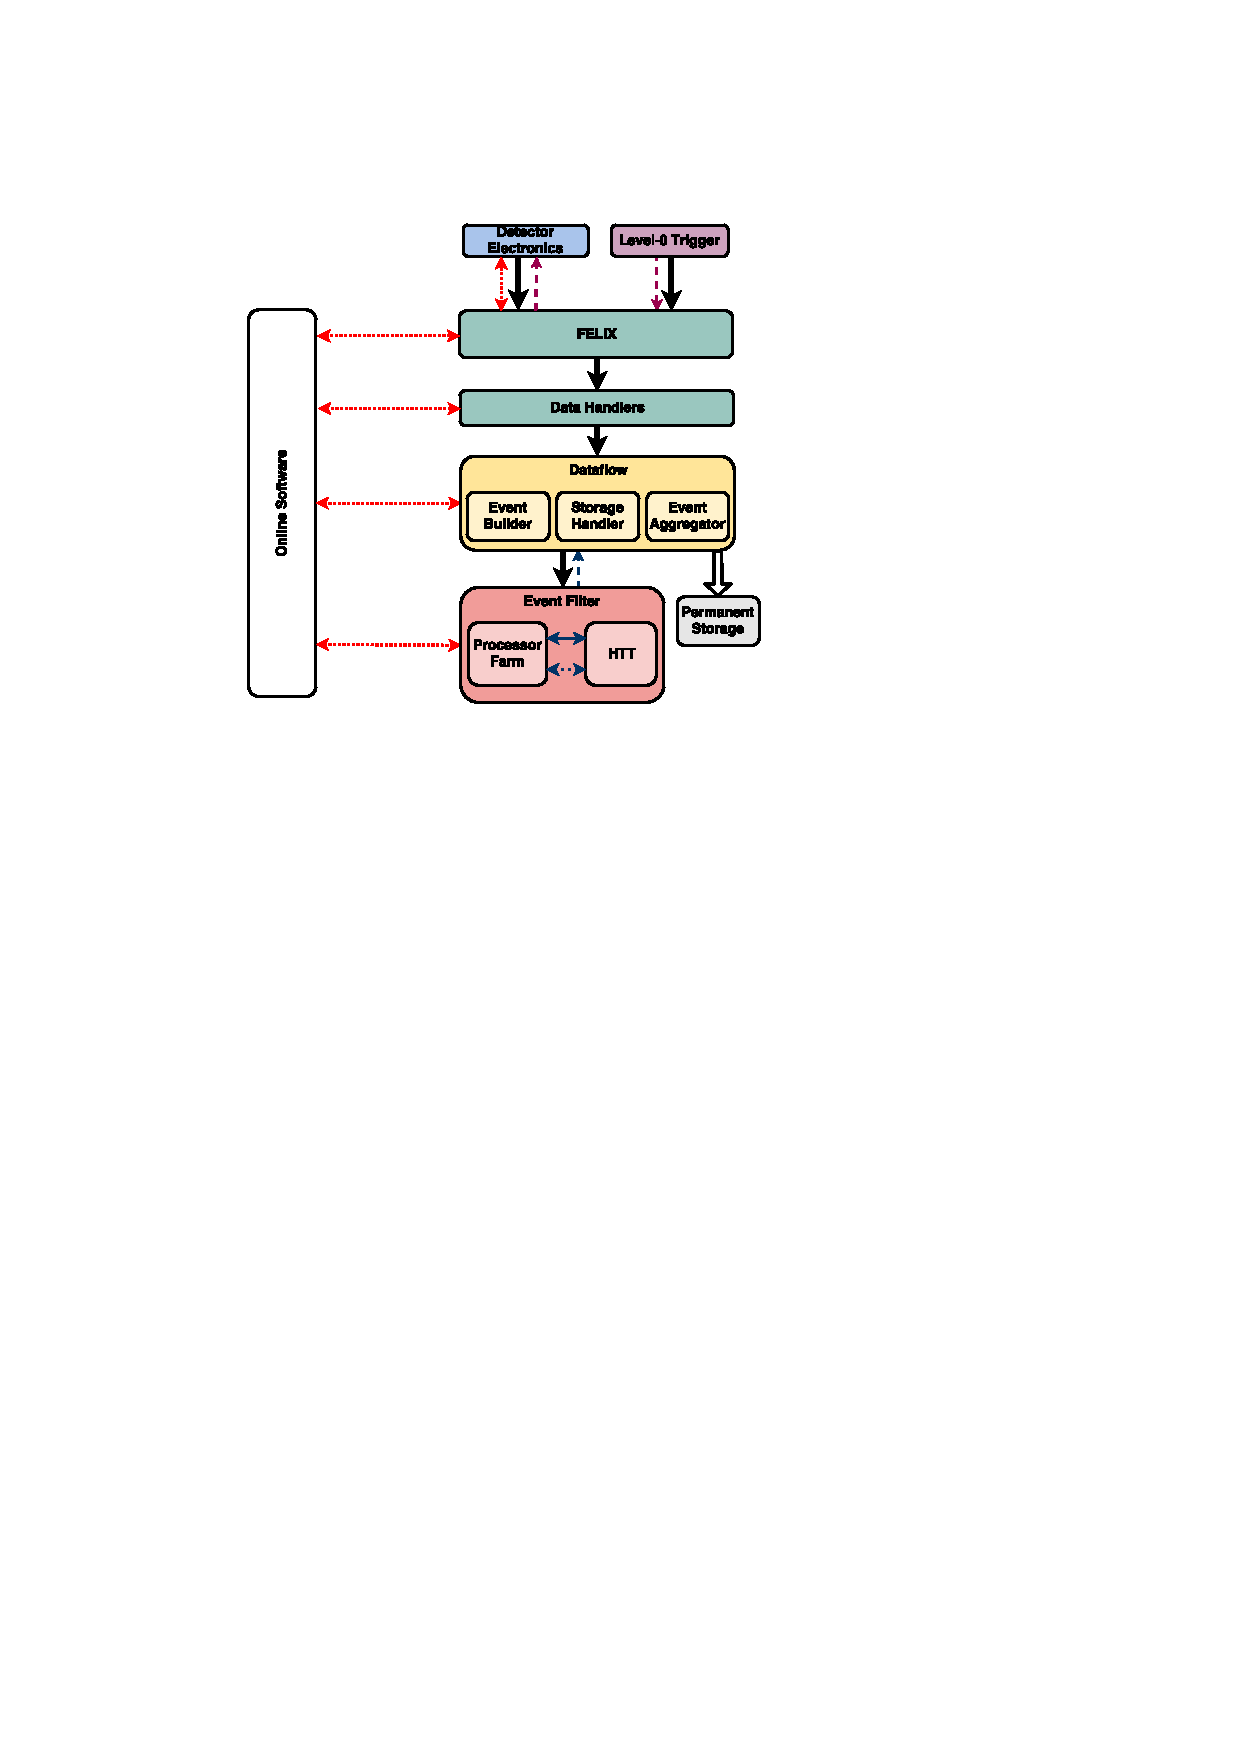
\includegraphics[height=7cm]{fig/Intro/Phase2_EF.pdf}
\subcaption{Event FilterとDAQシステムの概要}
\end{minipage}%
\caption[高輝度LHC-ATLAS実験におけるTDAQシステムの概要]{高輝度LHC-ATLAS実験におけるTDAQシステムの概要\cite{tdr_phase2tdaq_2017020}。 (a)にLevel-0 Triggerシステムの概要を示す。Level-0 TriggerはLevel-0 CaloとLevel-0 Muonに大別され、それぞれCTPで総合的なトリガー判定がなされる。CTPで後段に送られるべきと判断された場合、FELIXを経由して各フロントエンドエレクトロニクスにL0A信号が分配される。 (b)にEvent FilterとDAQシステムの概要を示す。L0Aを受けた各システムは検出器からのヒットデータをFELIXに送る。FELIXは受け取ったデータをEvent Filterに渡す。EFではソフトウェアベースのトリガー判定が行われ、最後まで残ったデータがCERNのPermanent Strageに保存される。}
\label{Phase2_TDAQ}
\end{figure}

L0 TriggerはL0 Calo、L0 Muon、Global Trigger、CTPで構成される。L0 Muonでは、新たに精密測定用のMDTもトリガーに用いられるようになる。TGCやRPCの情報と組み合わせることでより精度の高いトリガー判定を実現する。Global TriggerはL1 CaloとMUCTPIからの位置や\pt、\Et などの情報を基に、特徴的なトポロジーを持つ事象を選び出してCTPに送る。CTPはトリガーメニュー (図\ref{Phase2_Triggermenu}) に従い、各トリガー条件に指定されたプリスケーリングファクターを適用してトリガー判定を行う。各フロントエンドエレクトロニクスにはFront-End Link eXchange  (FELIX) を経由してLevel-0 Accept (L0A) 信号が分配される。L0Aを受けた各エレクトロニクスは該当する検出器のヒット情報をFELIXに送り返す。FELIXはこれらのデータをEvent Filterに転送する。Event Filterではソフトウェアのトリガー判定が行われトリガーレートは10 kHzまで削減される。最終的に残ったデータは、CERNの永久ストレージに保存される。

\begin{figure} 
\centering
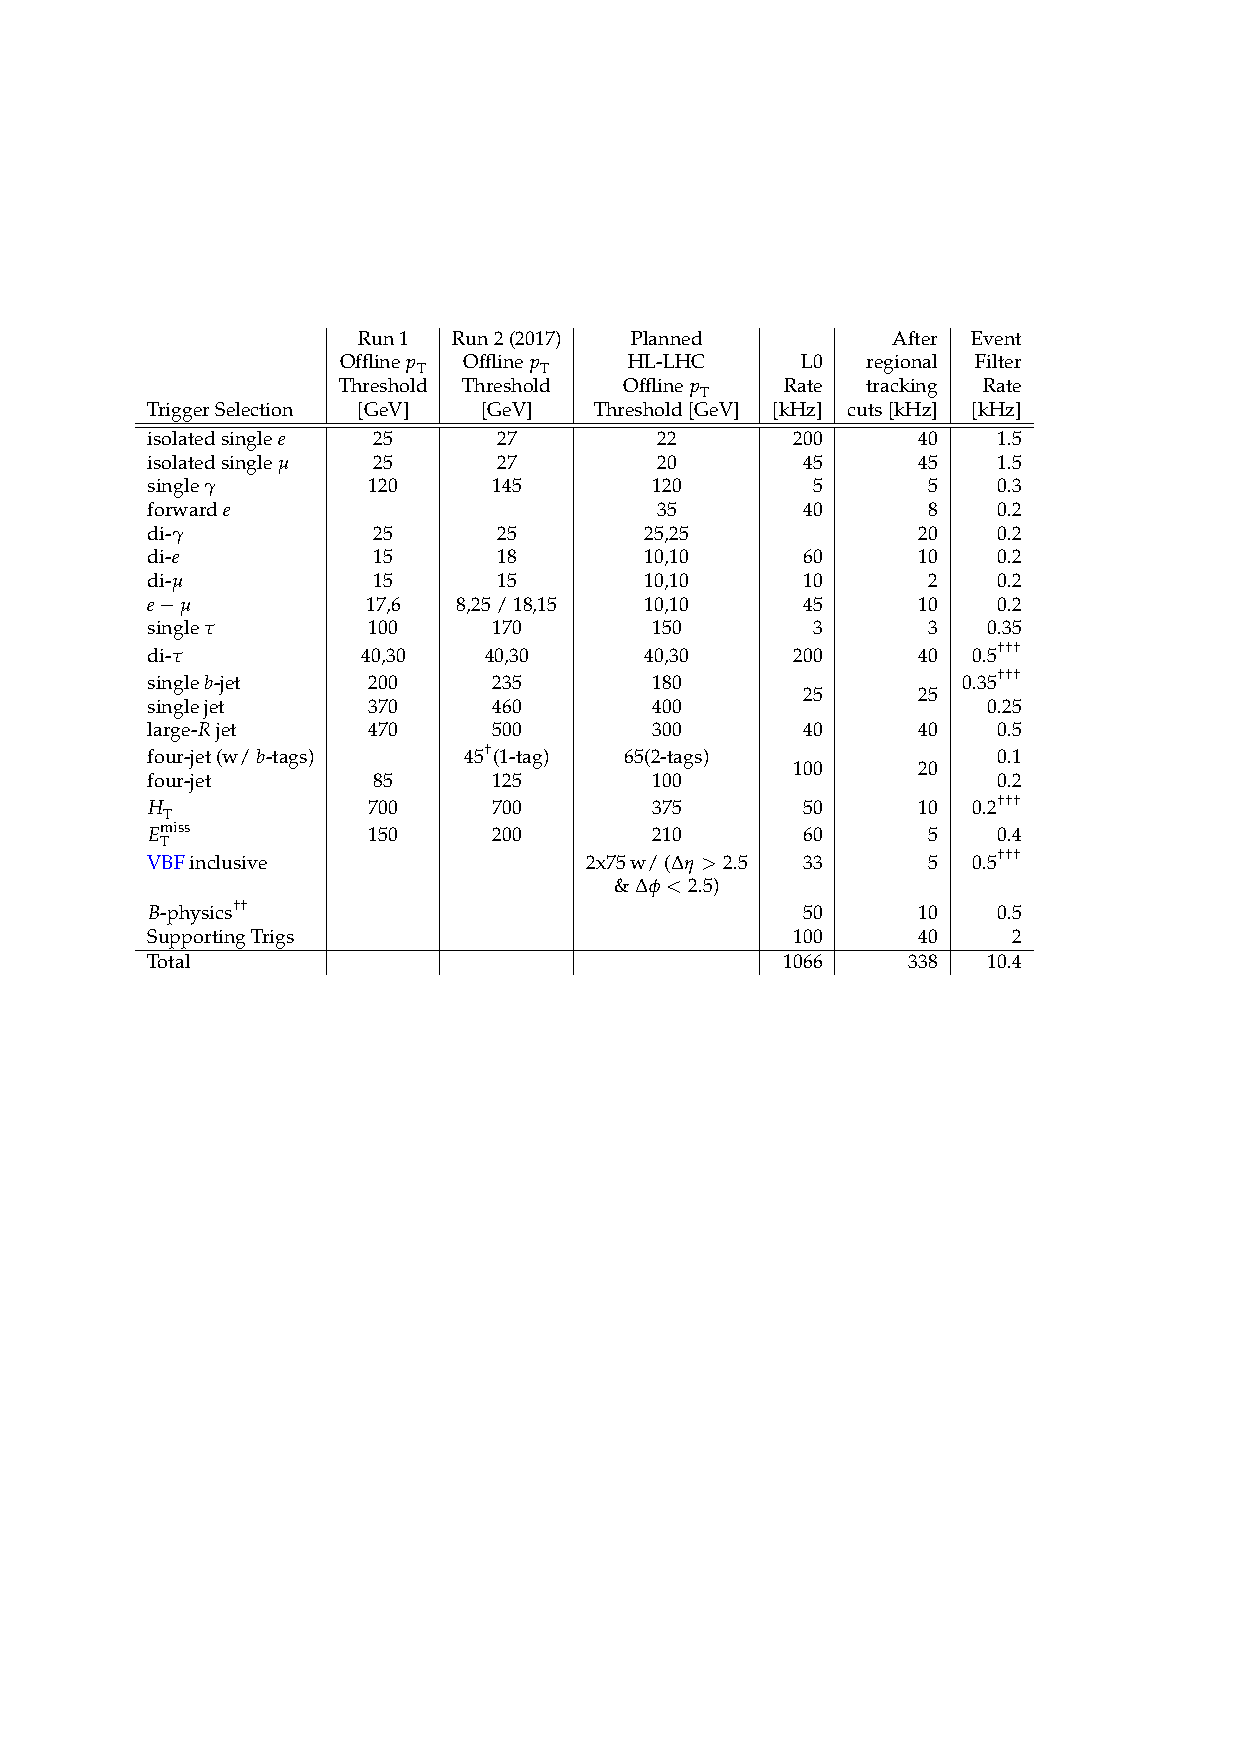
\includegraphics[width=16cm]{fig/Intro/Phase2_Triggermenu.pdf}
\caption[高輝度LHCにおけるトリガーメニューの例]{高輝度LHCにおけるトリガーメニューの例\cite{tdr_phase2tdaq_2017020}。解析に利用される典型的なオブジェクトに対してL0 TriggerおよびEvent Filterでのトリガーレートが分配されている。L0 TriggerレートはRun3の約10倍、Event Filterでのレートは約6倍に増強される。}
\label{Phase2_Triggermenu}
\end{figure}


\section{TGC検出器トリガーシステム}
\label{sec_TGCtrigger}

    \subsection{TGCトリガーのコンセプト}
    \label{subsec_trigger_concept}
本節では本研究のテーマであるTGC検出器のトリガーシステムについて述べる。
衝突点からエンドキャップ方向  (1.05 < |$\eta$| < 2.4) に飛来するミューオンはエンドキャップトロイド磁石で曲げられ、TGC検出器に入射する。TGC検出器の各層ではワイヤー、ストリップによる2次元読み出しで、TGCを通過したミューオンの  (R、$\phi$) 座標を検出する。TGC検出器はz方向に3つのステーションを持っており、ステーション間のコインシデンスをとることでミューオンの3次元飛跡を再構成し、それをもとに運動量を概算する。TGC検出器での運動量概算手法のコンセプトを図\ref{TGC_triggerconcept}に示す。

\begin{figure} 
\centering
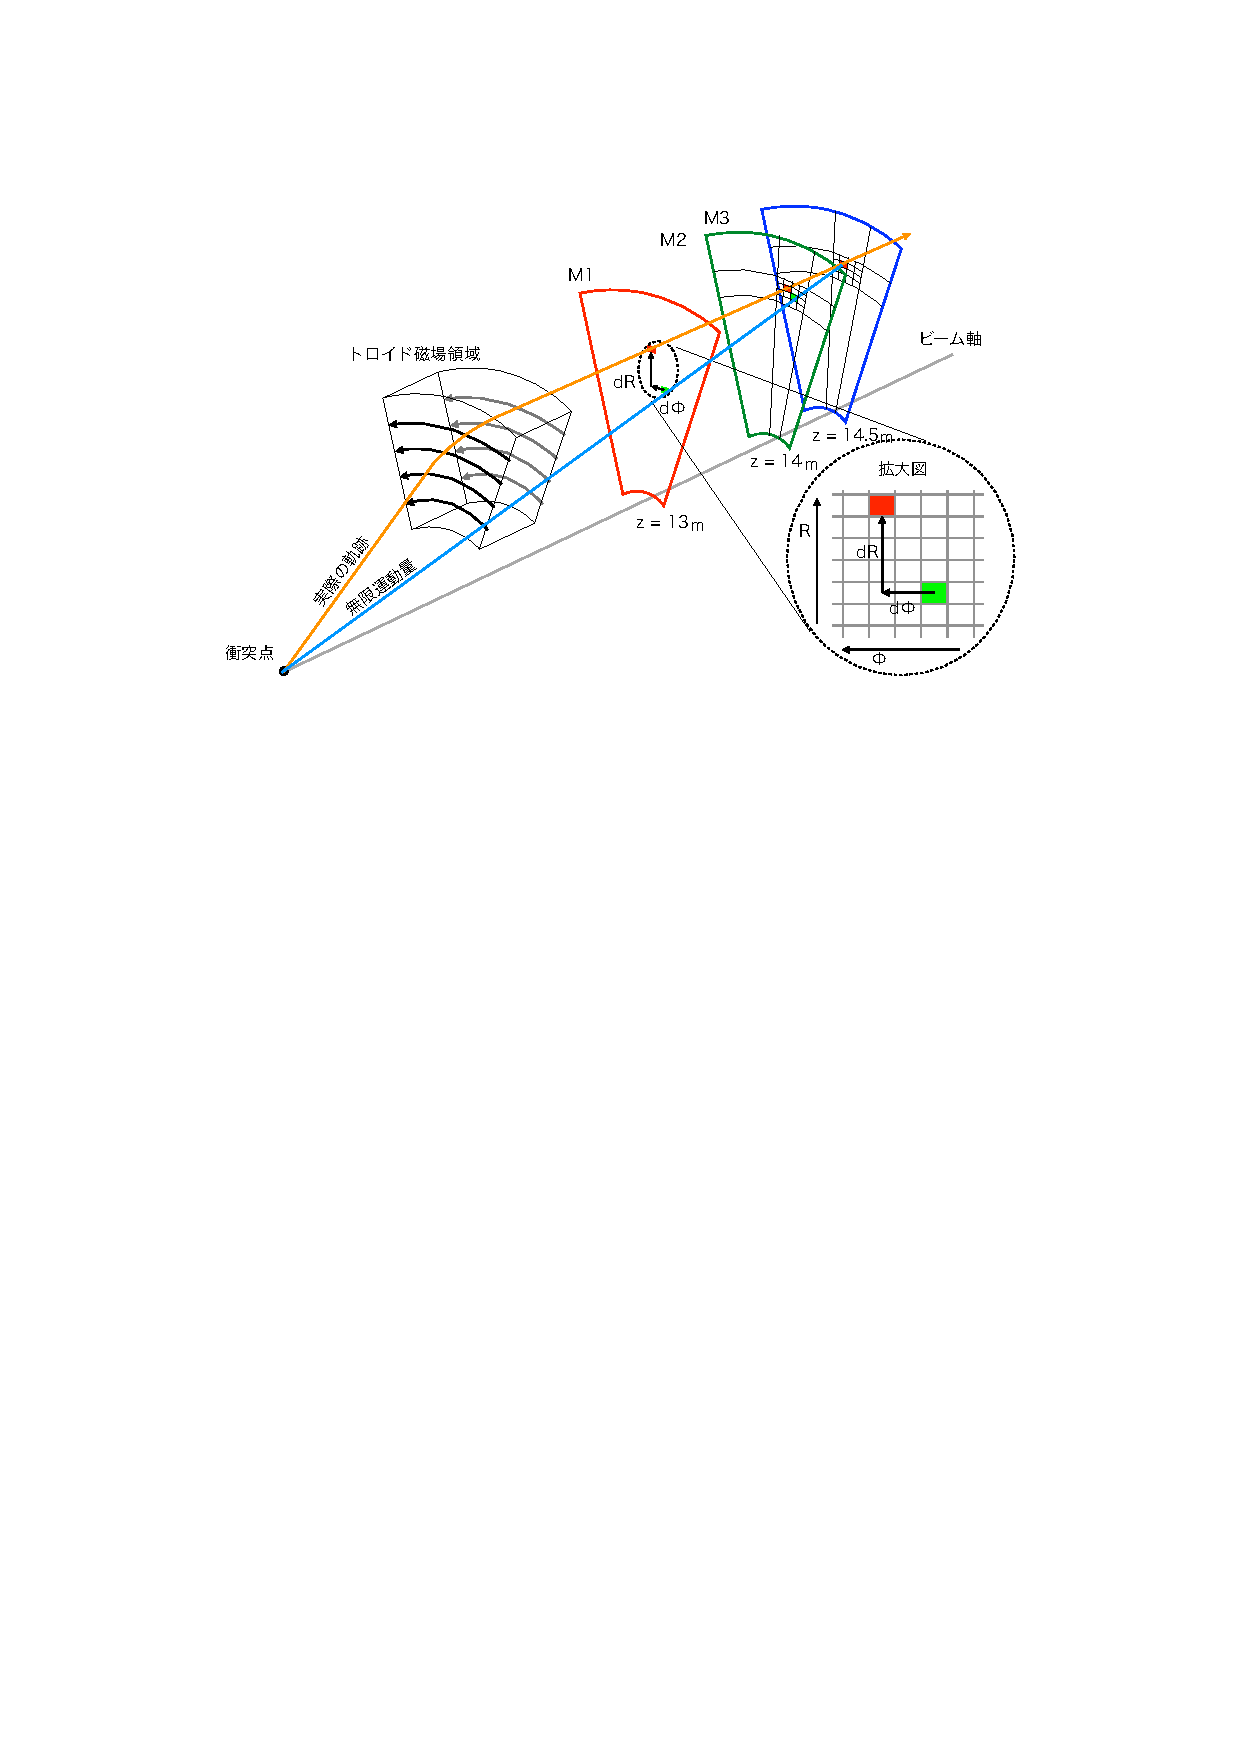
\includegraphics[width=16cm]{fig/Intro/TGC_triggerconcept.pdf}
\caption[TGCにおけるトリガーのコンセプト]{TGCにおけるトリガーのコンセプト\cite{mt_akatsuka}。ミューオンが実際に残したヒット点と無限運動量飛跡の位置の差分 ($\mathrm{dR}$,$\mathrm{\phi}$)を利用して\pt を概算する。}
\label{TGC_triggerconcept}
\end{figure}

内部飛跡検出器では、磁場で曲げられた粒子の曲率半径を利用して運動量を測定する。一方で、TGC検出器自体は磁場領域の外にあり、ミューオンは検出器を直線的に通過するため、この手法は利用できない。そこでTGC検出器では、3つのステーションのヒットから再構成したミューオンの飛跡と、M3のヒット点と衝突点を直線的結んだ無限運動量飛跡の"なす角"を分別変数に利用して、\pt を概算する。具体的にRun3のロジックでは、ミューオンが実際に残したヒット点と無限運動量飛跡のM1及びM2の交点との位置の差分  ($\mathrm{dR}$ , $\mathrm{d\phi}$)を 利用する\footnote{高輝度LHC-ATLAS実験では実際の飛跡と無限運動量飛跡のなす角($\mathrm{\Delta\theta, \Delta\phi}$)が利用される。本質的に等価なロジックである。}。\pt が小さいミューオンほどトロイド磁場領域で大きく曲げられるため、$\mathrm{dR}$ 、 $\mathrm{d\phi}$は大きくなる。
\ref{}節で述べたようにエンドキャップトロイド磁石から作られる磁場とバレルトロイド磁石で作られる磁場は互いに干渉しており、エンドキャップ領域に張られる磁場は、$\phi$方向の成分だけでなくR方向にも成分をもつ。そのため衝突点から飛来するミューオンはR方向だけでなく$\phi$方向にも曲げられる。また磁場が一様でないため、 ($\mathrm{dR}$ , $\mathrm{d\phi}$)と\pt の関係はミューオンの飛来する場所に依存する複雑な関数となり、代数的に求めるのが困難である。そこでシミュレーションを用いて、あらかじめ  ($\mathrm{dR}$ , $\mathrm{d\phi}$) と\pt の関係性をまとめたテーブル  (Look Up Table、LUT) を領域ごとに用意することで、迅速に\pt を計算している。

\begin{figure} 
\centering
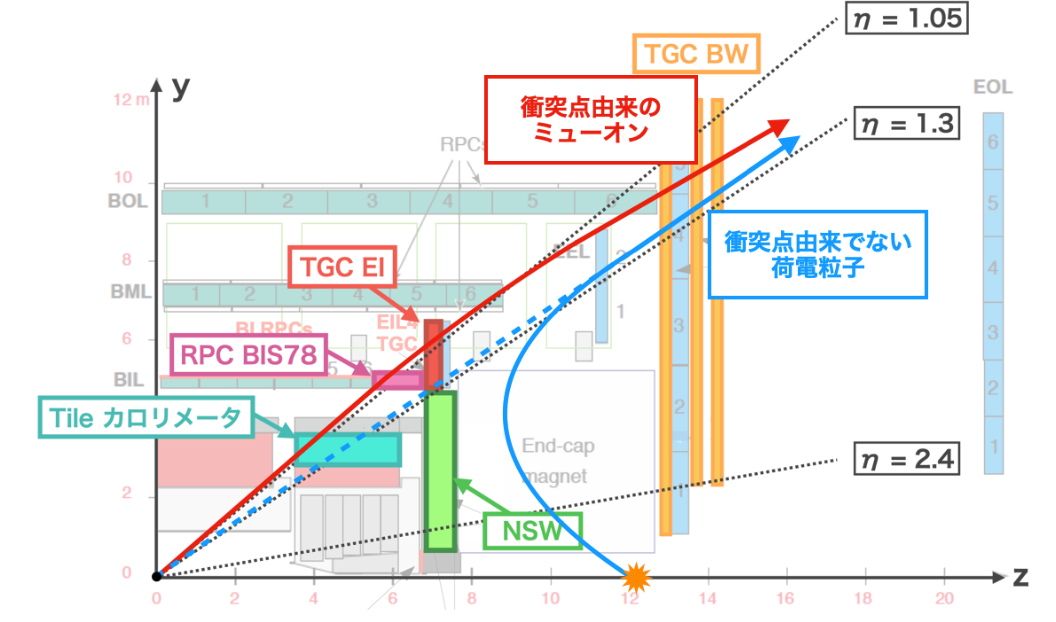
\includegraphics[width=16cm]{fig/Intro/TGC_Inner_concept.png}
\caption[フェイクトリガーの例]{Inner Coincidenceで落とすことが期待されるフェイクトリガーの例\cite{mt_kawamoto}}

\label{TGC_Inner_concept}
\end{figure}

加えてRun2以降のトリガーロジックでは、TGC BWの情報から再構成されたミューオンの情報とエンドキャップトロイド磁場内部にある検出器で得られた情報のコインシデンスがとられる。このコインシデンスをInner Coincidenceと呼ぶ。これにより、図\ref{TGC_Inner_concept}に示されるような、"フェイクトリガー"と呼ばれる衝突点に由来しない荷電粒子をトリガーしてしまう事象を減らすことができる。衝突点に由来しない荷電粒子が生成される例として、陽子陽子衝突やハドロンカロリメーター内で生成される中性ハドロンが、エンドキャップトロイド磁石と相互作用することで荷電粒子を放出される場合などが挙げられる。実際に、Inner Coincidenceが取られていなかったRun1のTGCシステムははフェイクトリガーを多く発行していたことが知られる。図\ref{TGC_faketrigger}にRun1でのミューオントリガー発行数の$\eta$分布を示す。1.05 < |$\eta$|のTGCがトリガーを発行する領域において、オフラインで再構成されたミューオンよりはるかに多くのトリガーが発行されていることがわかる。この差がフェイクトリガーであると考えられる。L1トリガーレートには上限があるため、フェイクトリガーによりトリガーレートを割いてしまうと、真に興味のある事象に対するアクセプタンスを減らすことにつながる。そのためフェイクトリガーの削減は、TGCのトリガーシステムにおいて重要な役割を果たす。
またNSWのような位置分解能に優れた検出器からの情報も組み合わせて\pt を計算することで、TGC BW単体での計算よりも精度を高めることができる。
この\pt に対して閾値を設け、それ以上の\pt を持つミューオンを含む事象を選別し、後段に送信する。

\begin{figure} 
\centering
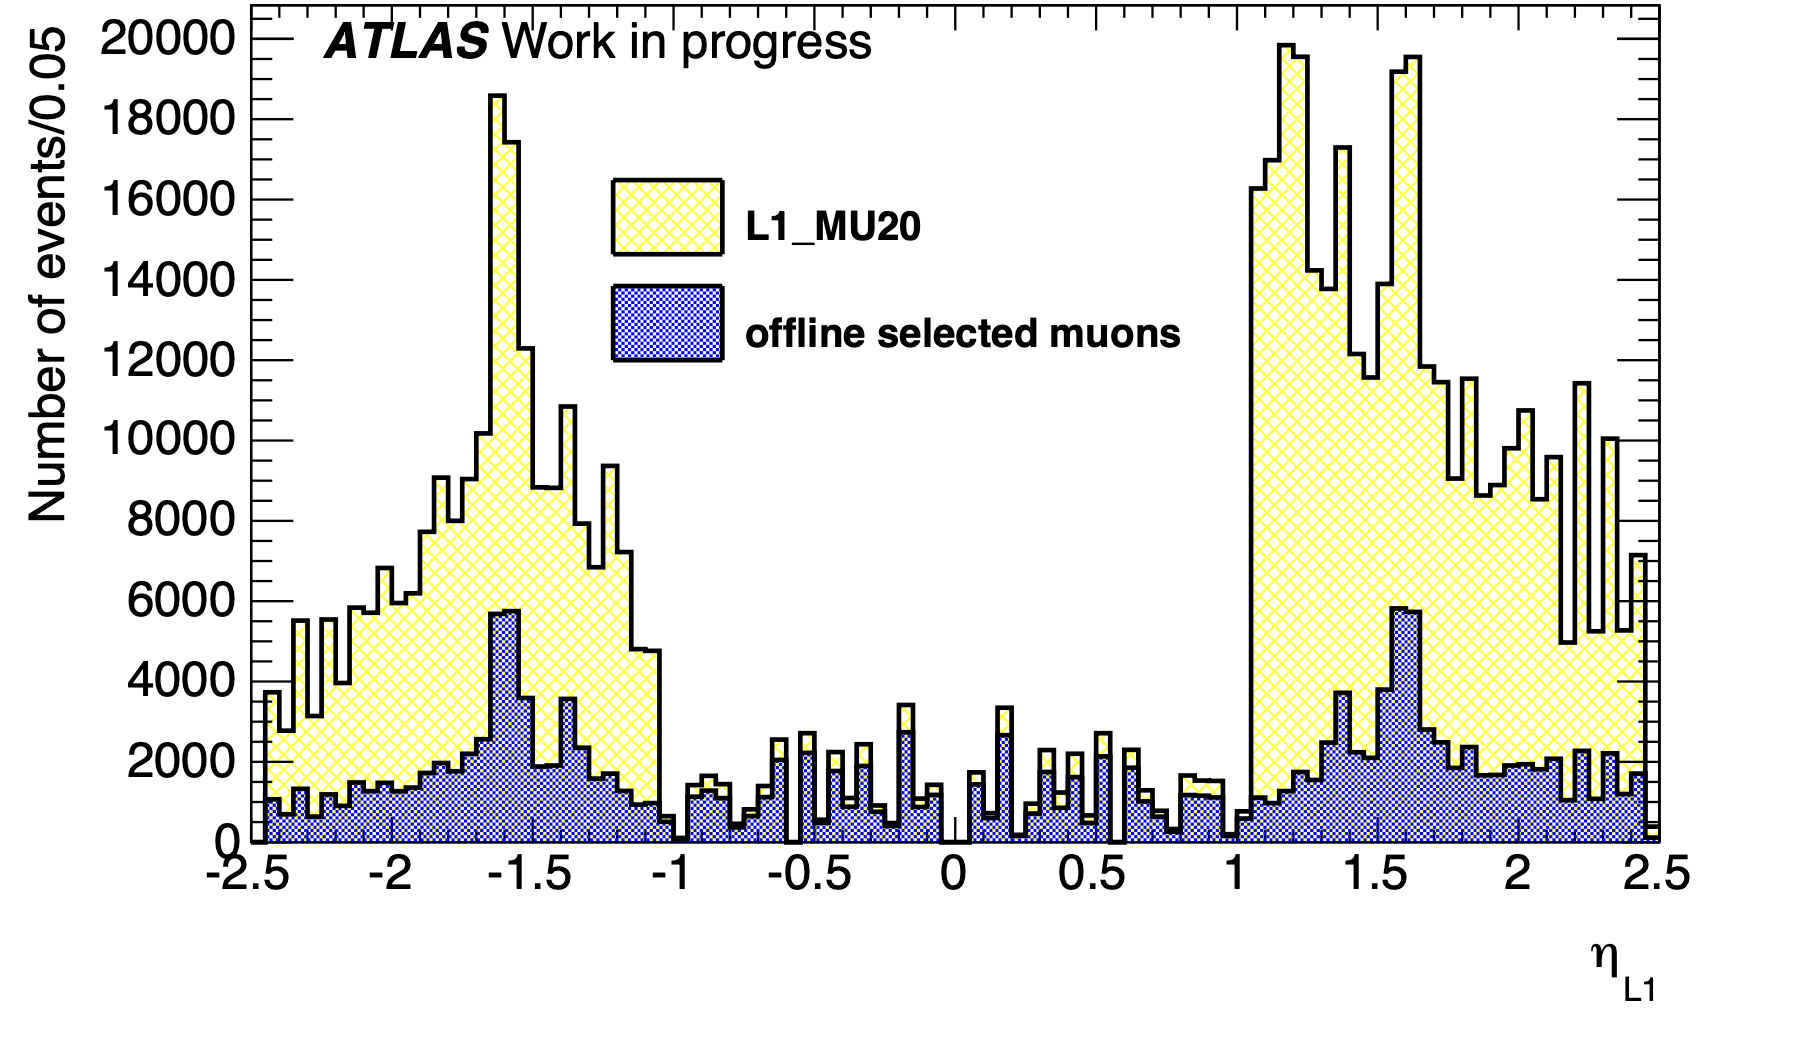
\includegraphics[width=16cm]{fig/Intro/TGC_faketrigger.png}
\caption[Run-1での\pt 閾値]{Run-1での\pt 閾値20 GeVのL1vel-1ミューオントリガーの発行数の$\eta$分布。}
\label{TGC_faketrigger}
\end{figure}



    \subsection{Run3でのTGCトリガーシステム}

\begin{figure} 
\centering
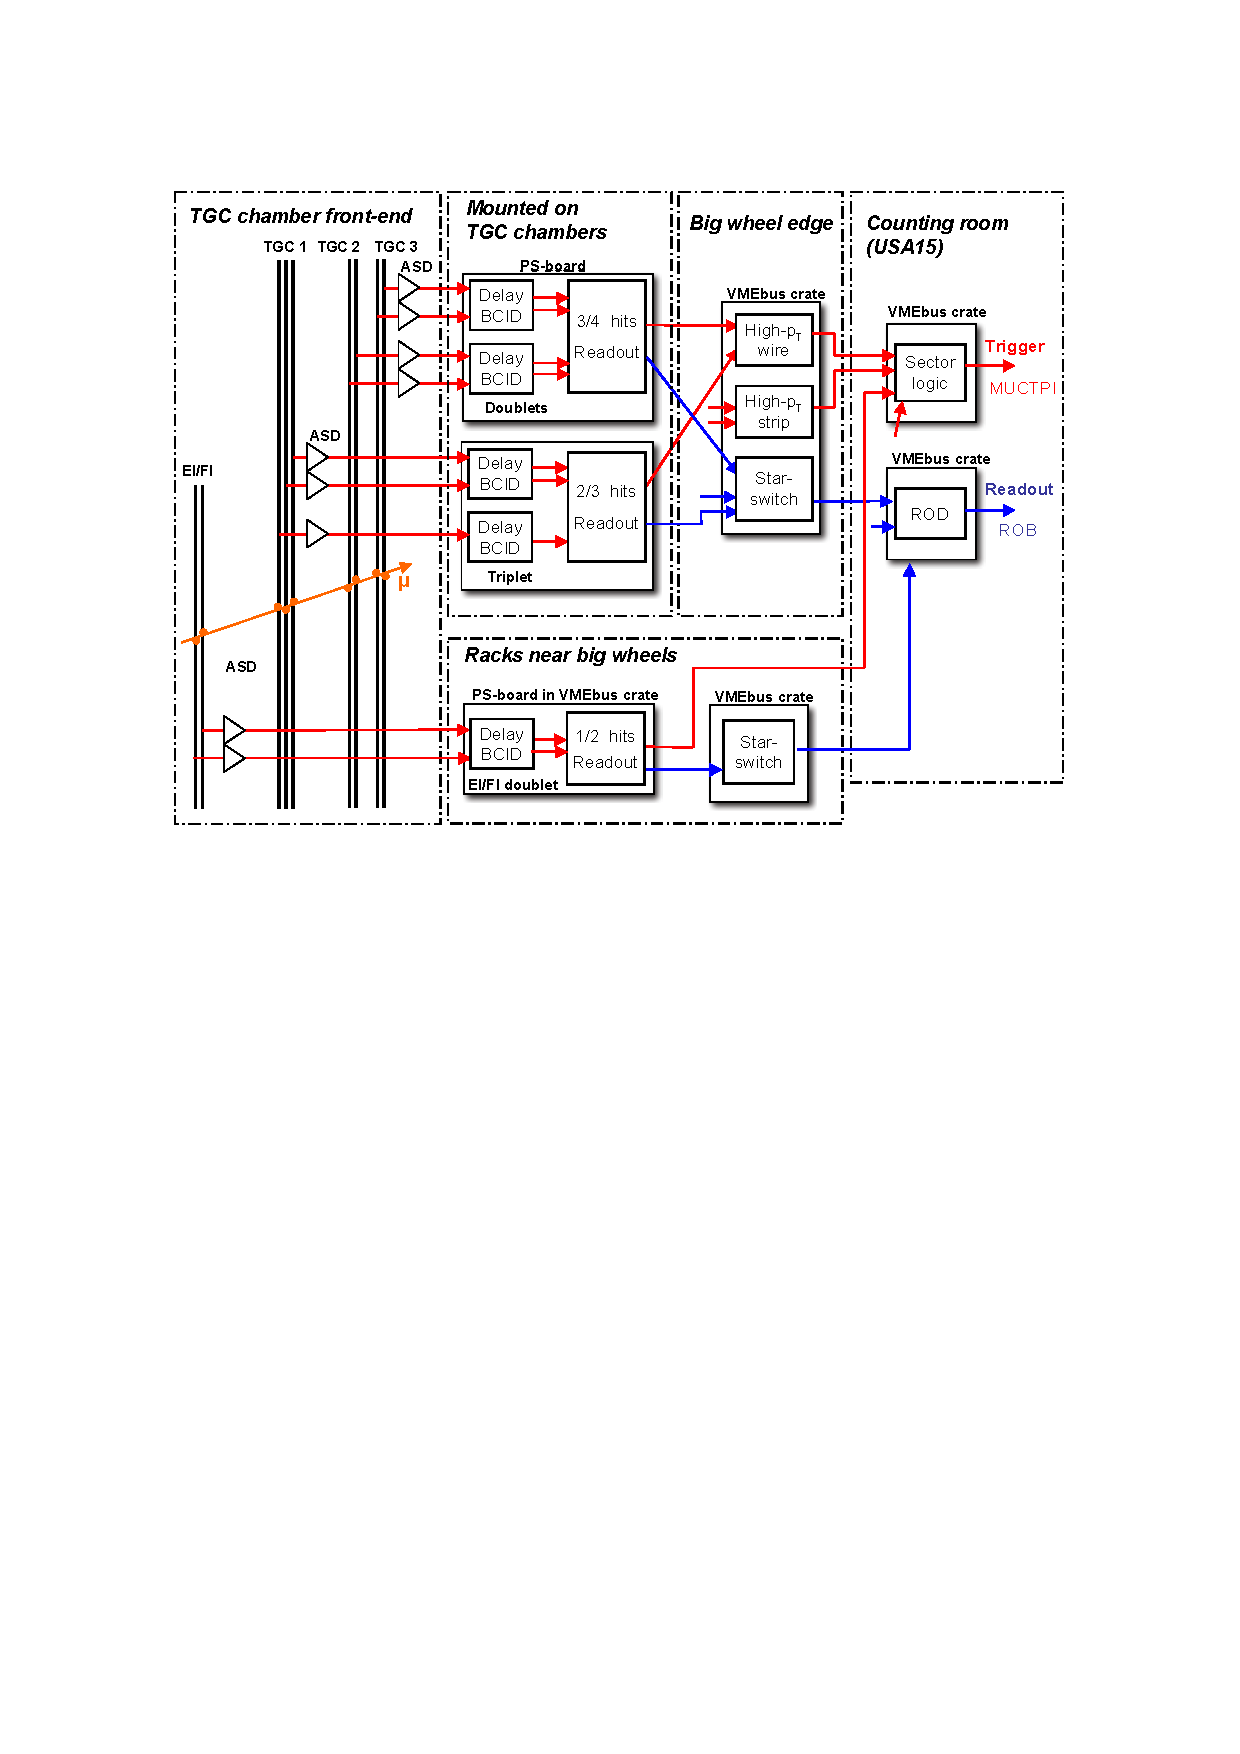
\includegraphics[width=16cm]{fig/Intro/TGC_run3tdaq.pdf}
\caption[Run3におけるTGC TDAQシステム]{Run3におけるTGC TDAQシステム}
\label{TGC_run3tdaq}
\end{figure}

上記のトリガーコンセプトを実現する現行 (Run3) のTGC TDAQシステムのブロック図を図\ref{TGC_run3tdaq}に示す。図の赤色の線はトリガーパス、青色はデータパスを示す。TGC検出器にミューオンが入射すると、各ガスレイヤーに張られたワイヤーとストリップでアナログの電流信号が発生する。アナログ信号はTGC検出器に直接取り付けられたAmplifier Shaper-Discriminator  (ASD) に集められる。ASDは信号を電圧信号に変換し増幅したのち、閾値電圧と比較することでデジタル信号を生成する。デジタル信号は後段のPS board上に搭載されたPatch-Panel ASIC  (PP ASIC) において、どのバンチ陽子衝突に由来するものか識別される  (BCID) 。この後から信号はトリガーパスとリードアウトパスに分けられる。

トリガーパスは、Slave Board  (SLB) ボード、High-pt  (HPT) ボード、Sector Logic  (SL) というパスを経由して後段に渡される。SLBではワイヤーとストリップそれぞれでM1ステーション内コインシデンスが取らる。またM2、M3ステーション間のコインシデンスもとられ、無限運動量飛跡との位置の差分、 ($\mathrm{dR_{23}}$,$\mathrm{d\phi_{23}}$)が計算される。この際、M1では3層中2層以上のヒット、M2、M3では4層中3層以上のヒットが要求され、コインシデンスが取れたもののうち$\mathrm{dR_{23}}$が小さいものを選択して出力する。HPTボードではM1とM3のコインシデンスにより ($\mathrm{dR_{13}}$,$\mathrm{d\phi_{13}}$)が計算され、絶対値の小さいものが優先的に出力される。SLボードではM3におけるヒット位置および ($\mathrm{dR_{13}}$,$\mathrm{d\phi_{13}}$)をもとにワイヤー・ストリップ間のコインシデンスがとられ、LUTを用いて\pt を概算する。また磁場内部に位置する検出器 (NSW、RPC BIS78、TGC EI、Tile カロリメーター)の飛跡情報とのコインシデンスもとられ、より精度の高い\pt が計算される。SLで得られた入射位置と\pt 情報はMUon-to Central Trigger Processor Interface  (MUCTPI) に送られ、CTPへ渡される。CTPで後段へ送るべきと判断された場合にはL1A信号が発行される。

読み出しパスはSLB、Star SWitch  (SSW) ボード、ReadOut Driver  (ROD) というパスを経由して後段へ渡される。PP ASICで同期された信号は、トリガー判定が完了するまでSLB内のL1 Bufferに保存される。SLBでは最大128イベント分の信号をバッファリングすることが可能である。前節で述べた通り、L1 TriggerはFixed latency Schemeを採用しており、L1 Bufferにデータが入ってからそのイベントにL1Aが出されるまでの時間  (L1 latency) は固定されている。そのためSLBはL1Aを受信した後、L1 latencyだけ前のデータを読み出すことで、正しくデータを読み出すことができる。SLBから読み出されたデータはSSWボードでゼロサプレスと呼ばれるデータ圧縮が行われ、イベント毎にパッケージされる  (Event Building)。RODは1つのセクター内の全てのSLB-SSWから送られたデータ集約し、さらに後段のReadOut System  (ROS) へとデータを送信する。

これらのTGCエレクトロニクスのうち、ASD、PS board、HPT、SSWはATLAS実験室内に設置され、フロントエンドエレクトロニクスと呼ばれる。図\ref{TGC_elec_mount}にフロントエンドエレクトロニクスの設置場所を示す。ASDはTGCチェンバーに直接取り付けられたアダプタボードにマウントされる。PS boardは2枚ごとにアルミケース  (PS-pack) に収納され、TGCチェンバー付近に設置される。HPTおよびSSWはBWの外側にあるMini-Rack内のVMEクレートに収められる。SL、ROD以降のエレクトロニクスはUX15から100 mほど離れたUSA15というATLAS回路室内に設置され、バックエンドエレクトロニクスと呼ばれる。HPTとSLおよびSSWとRODの通信はUX15とUS15間の限られた帯域幅を用いて行われる必要があり、Run3ではG-linkと呼ばれる旧式のシリアル通信規格で接続される。G-linkにおけるシリアルデータ転送レートはおよそ1 Gpbsである。

\begin{figure} 
    \centering
    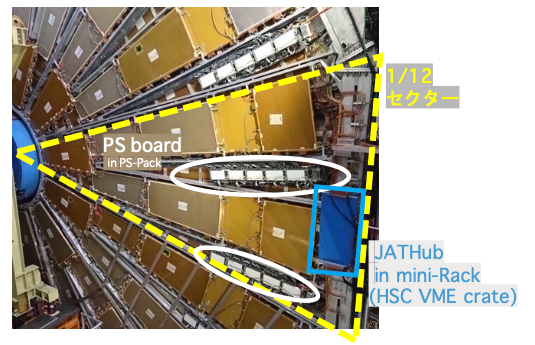
\includegraphics[width=16cm]{fig/Intro/TGC_elec_mount.png}
    \caption[TGCエレクトロニクスが設置されている場所]{TGCエレクトロニクスが設置されている場所}
    \label{TGC_elec_mount}
\end{figure}

次にTTC系について述べる。Level1 Bufferより前の読み出し回路およびトリガー回路は、Fixed latency schemeを実現するためLHCの陽子バンチ衝突と同期して動作する必要がある。この同期のために、各検出器とLHCを同期させるシステムをTiming, Trigger and Control  (TTC) システムとよび、そのために配布される信号をTTC信号と呼ぶ。TTC信号には陽子バンチ衝突と同期した40.079 MHzのLHCバンチ交差クロック  (LHCクロック) やL1A信号などが含まれる。Run3におけるTTC系の概要を図\ref{Run3_TTC}に示す。TTC信号はCTPから各検出機サブシステムのLocal Trigger Processor  (LTP) に配られる。その後TTC信号はTTCvi、TTCex、TTXrxと呼ばれるTTC専用モジュールおよび専用線を通じて、PS board、HPT、SSW、SLへ分配される。

\begin{figure} 
\centering
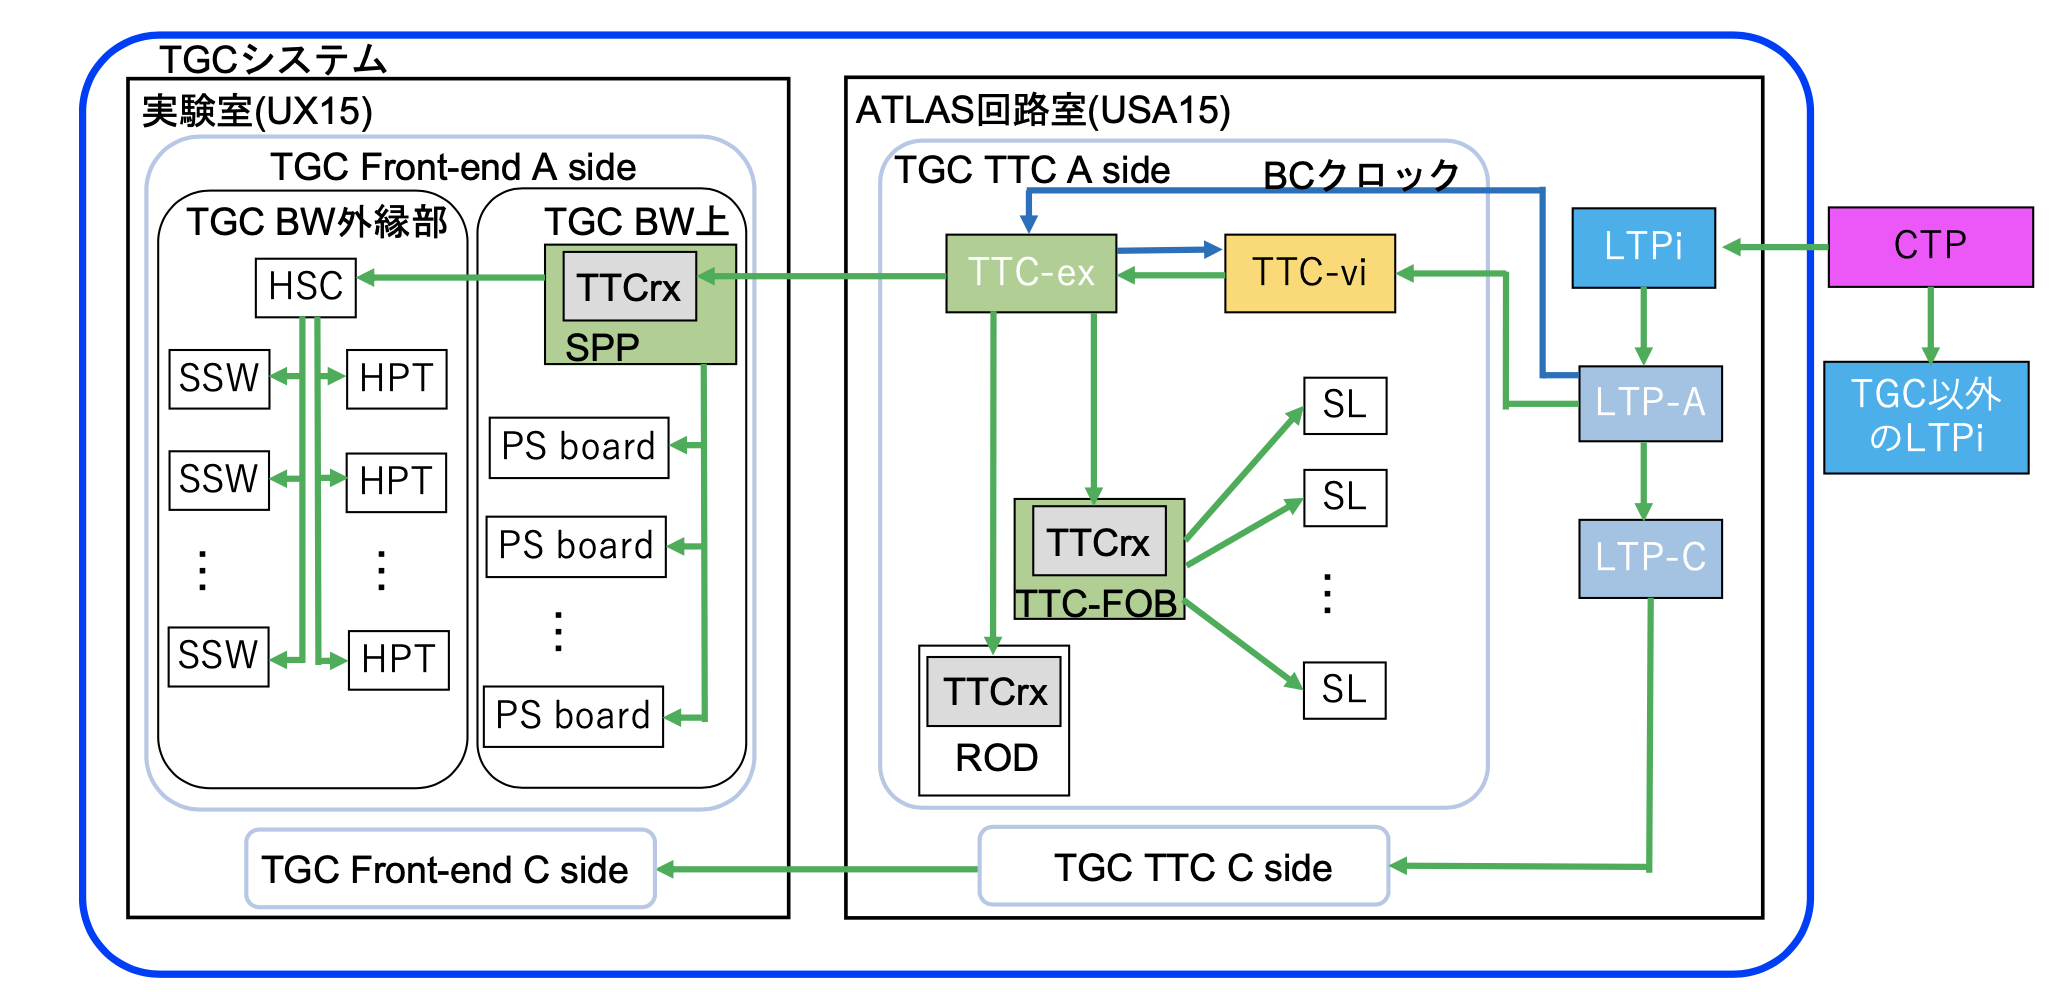
\includegraphics[width=16cm]{fig/Intro/Run3_TTC.png}
\caption[Run3 TGCシステムにおけるTTCシステムの概要]{Run3 TGCシステムにおけるTTCシステムの概要\cite{JINST:2008}}
\label{Run3_TTC}
\end{figure}

以上に述べたRun3のTDAQシステムでは、高輝度LHC-ATLAS実験のトリガーおよび読み出し性能の要求を満たすことができない。この限界は、主にSLBに設置されるL1 Bufferの容量と、ATLAS実験室と回路室間の帯域幅に由来している。Run3では、L1 Bufferは最大128イベント分のデータしか保存できないため、高輝度LHC-ATLAS実験のL0 latencyの要求である10us  (400バンチ) の間データを保持することができない。さらに、1 MHzの初段トリガーレートに対応するデータ量を読み出すためには、現行システムのATLAS実験室と回路室間の帯域幅では不十分である。

    \subsection{高輝度LHC-ATLAS実験でのTGCトリガーシステム}  
前節で述べた問題を解決するため、高輝度LHC-ATLAS実験ではTGC検出器のエレクトロニクスシステムが大幅にアップグレードされる。主な違いはPS boardでBCIDされたすべてのヒット信号が、トリガーをかけられることなく後段のSLに送られることである。Run3のトリガーパスでは、検出器からの信号はSLBやHPTボードでのコインシデンスを通じて、データサイズを徐々に減らしながら回路室へ送られる。高輝度LHC-ATLAS実験では新しく高速シリアル通信技術を導入することで、実験室と回路室の間の帯域幅を1 Gbps程度から10 Gbpsへ大幅に拡張する。これにより、PS boardで受け取ったTGCからの信号を削減することなく、すべて回路室のSLへ転送することが可能になった。回路室では、ボードのサイズや放射線への耐性に対する制約が少ないため、バックエンドエレクトロニクスであるSLには大規模なFPGAを搭載することができる。その結果、CTPからL0Aが発行されるまでデータを保管しておくL0 Bufferも余裕を持って実装することができ、10 usのL0 latencyに対応することが可能である。またSLは1つのトリガーセクター内の全てのPS boardからのヒット信号を集約するため、TGC BW 7層分の情報を利用した、より包括的なトリガーアルゴリズムを実現することができる。高輝度LHC-ATLAS実験でのトリガーロジックの詳細は\ref{subsec_phase2_triggerlogic}節で示す。

図\ref{TGC_phase2tdaq}に高輝度LHC-ATLAS実験でのTGC検出器エレクトロニクスの概要を示す。ASDは現行システムのものを引き続き使用する。一方で、Run3で使われていたPS board、SLB、HPT、SLはすべて撤去され、新しくPrimary ProceSsor board  (PS board)、JTAG AssisTance Hub  (JATHub)、Endcap Sector Logic  (SL) が設置される。PS boardはRun3と同様にPS-packに格納され、TGC検出器付近に設置される。JATHubはMini-pack内のVMEクレートに設置される。SLはUSA15のATCAクレートに設置される。1つのSLはTGCの1/24セクター担当し、このセクターを担当する最大31枚のPS boardからヒットデータを受け取る。

\begin{figure} 
\centering
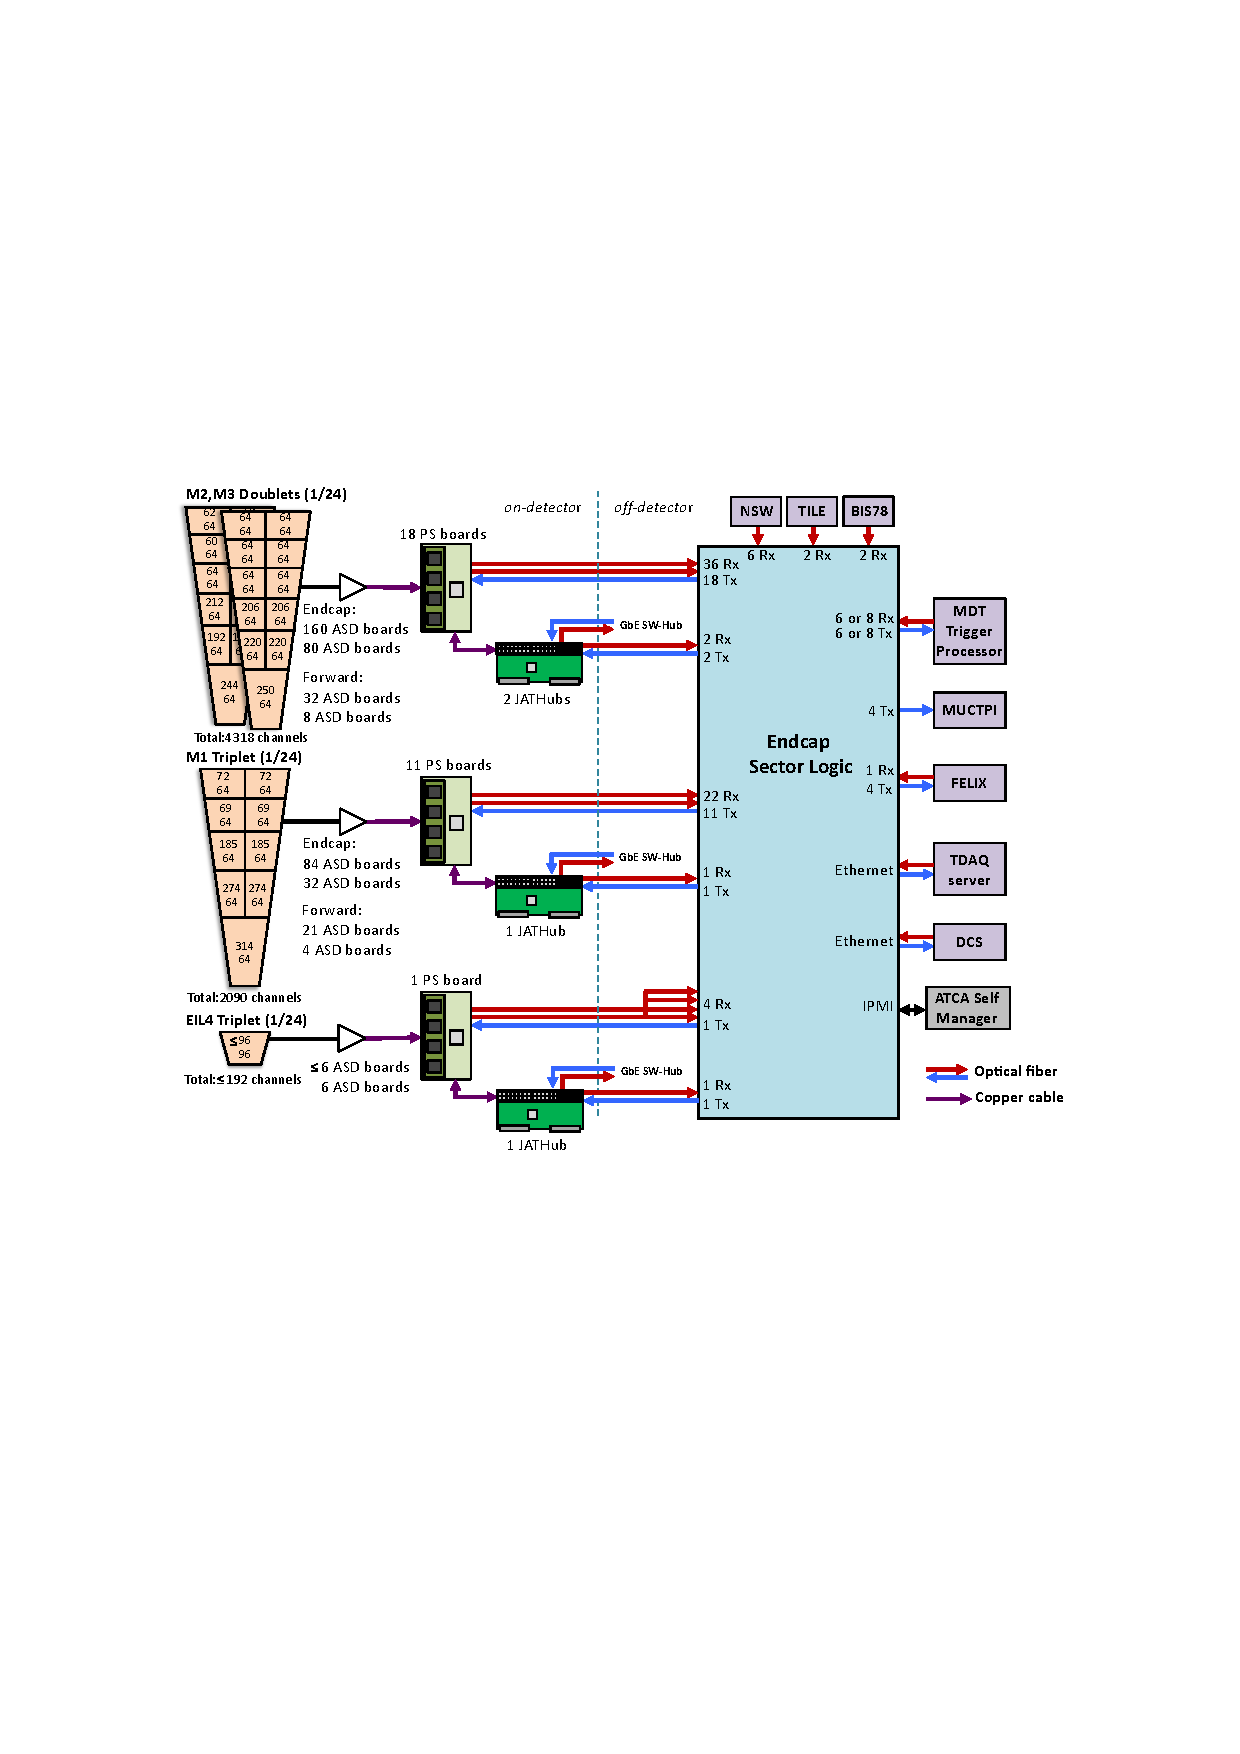
\includegraphics[width=16cm]{fig/Intro/TGC_phase2tdaq.pdf}
\caption[高輝度LHC-ATLAS実験におけるTGC検出器システムの概要]{高輝度LHC-ATLAS実験におけるTGC検出器システムの概要\cite{tdr_phase2muon_2017017}}
\label{TGC_phase2tdaq}
\end{figure}

トリガーパスにおけるデータ伝達を図中赤色の矢印で示す。TGCで生じる電流信号はASDでデジタル信号に変換された後、PS board上のPP ASICで陽子バンチ交差クロックと同期される。PP ASICからの信号は、ヒットの有無に関わらず、PS board上のFPGAから光ファイバーを通じてSLに送信される。SLは、PS boardから送られるTGC BW 7層の情報に加え、TGC BW、TGC EI、NSW、RPC BIS78、Tile カロリメーターの情報も用いてミューオンの\pt を概算する。その後SLはMDT Trigger Processorにミューオン飛跡候補を送信し、よりよい\pt 分解能の情報を得る。SLからのトリガー出力はMUCTPI通じてCTPへ送信される。CTPでのトリガー判定を待っている間のデータのバッファーもSLで行われる。SLはL0Aを受信すると、対応するイベントのデータをFELIXを通じて後段に送信する。

コントロールパスを青色で示す。SLは光ファイバーを通じてコントロール信号を送ることでPS boardを制御する。さらに、SLはCTPからFELIXを介して取得したTTC信号をこの線に乗せてPS boardに分配する。
このシステムではバックエンドのSLとフロントエンドのPS boardが光リンクのみで接続されており、
トリガー・データ読み出し、コントロール、TTCの分配を単純なセットアップで実現している。

以下にそれぞれのエレクトロニクスとその役割を説明する。

        \subsection*{Amplifier-Shaper-Discriminator (ASD)}
    ワイヤー、ストリップからの電流信号はTGCのチェンバーに直接取り付けらたAmplifier-Shaper-Discriminator  (ASD) ボードで電圧信号に変換された後に増幅され、閾値電圧との比較による信号識別を経て、最終的にLVDS規格のデジタル信号へ変換される。図\ref{TGC_ASD}にASDの概要を示す。ASDはチャージアンプである前段増幅器 (Preamplifier)、差動電圧増幅回路、コンパレーターから構成されている。前段増幅回路では、0.8 V/pのゲインで電流信号を電圧信号に変換する。その信号は差動電圧増幅回路で7倍に増幅され、コンパレーターで閾値電圧を超えている時間に対応するパルス長のLVDS信号に変換される。この閾値電圧はPS boardから設定できるようになっている。またASDにはTGCのチャージ出力をエミュレートするTest Pulse源が実装されており、ASD以降のトリガー・データパスのデバッグに利用される。1枚のASDボードには4枚のASDチップが搭載されており、1枚あたり4チャンネル、全部で16チャンネルの信号を処理する。TGCの読み出しチャンネルはおよそ32万チャンネルであるため、システム全体ではおよそ2万枚のASDボードが設置される。

    \begin{figure}
    \begin{minipage}[b]{.5\linewidth}
    \centering
    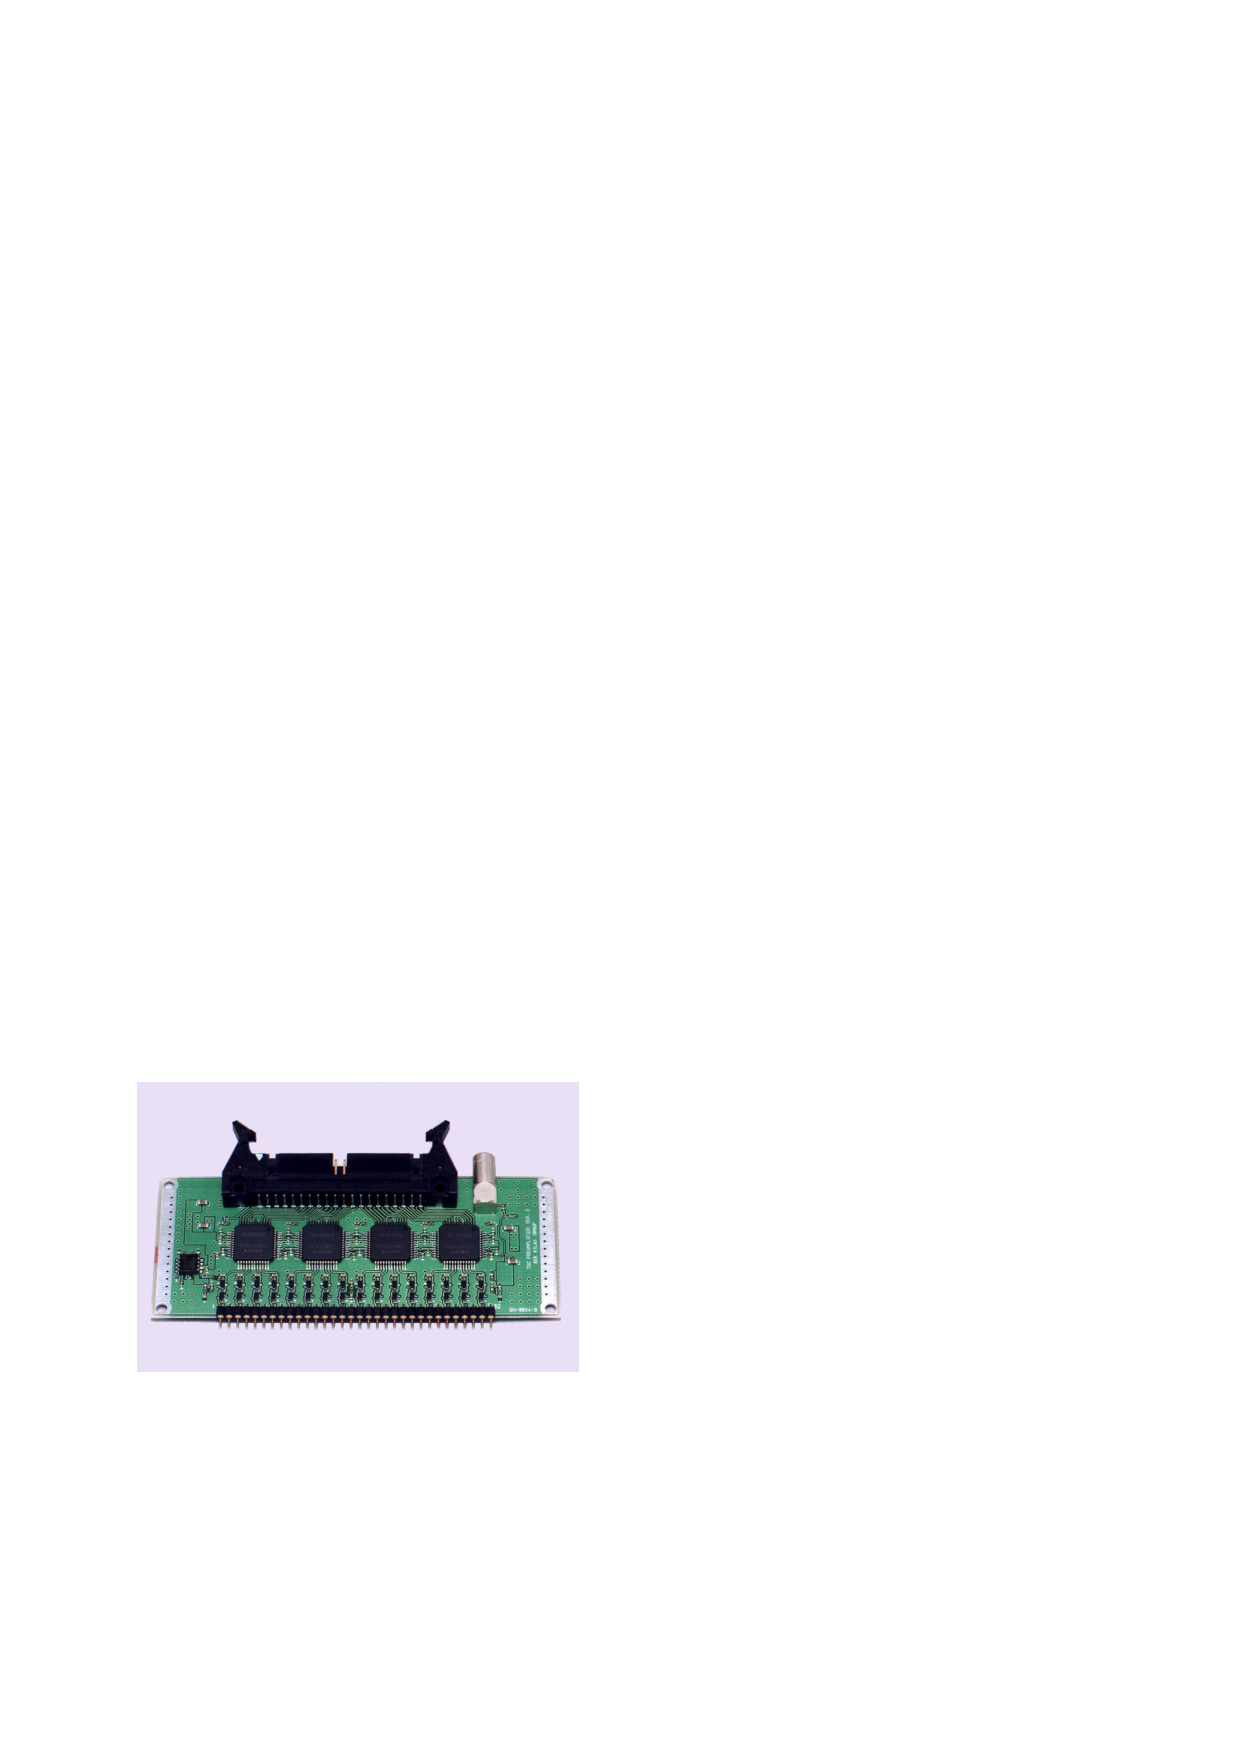
\includegraphics[height=5cm]{fig/Intro/TGC_ASD.pdf}
    \subcaption{ASDボードの写真}
    \end{minipage}%
    \begin{minipage}[b]{.5\linewidth}
    \centering
    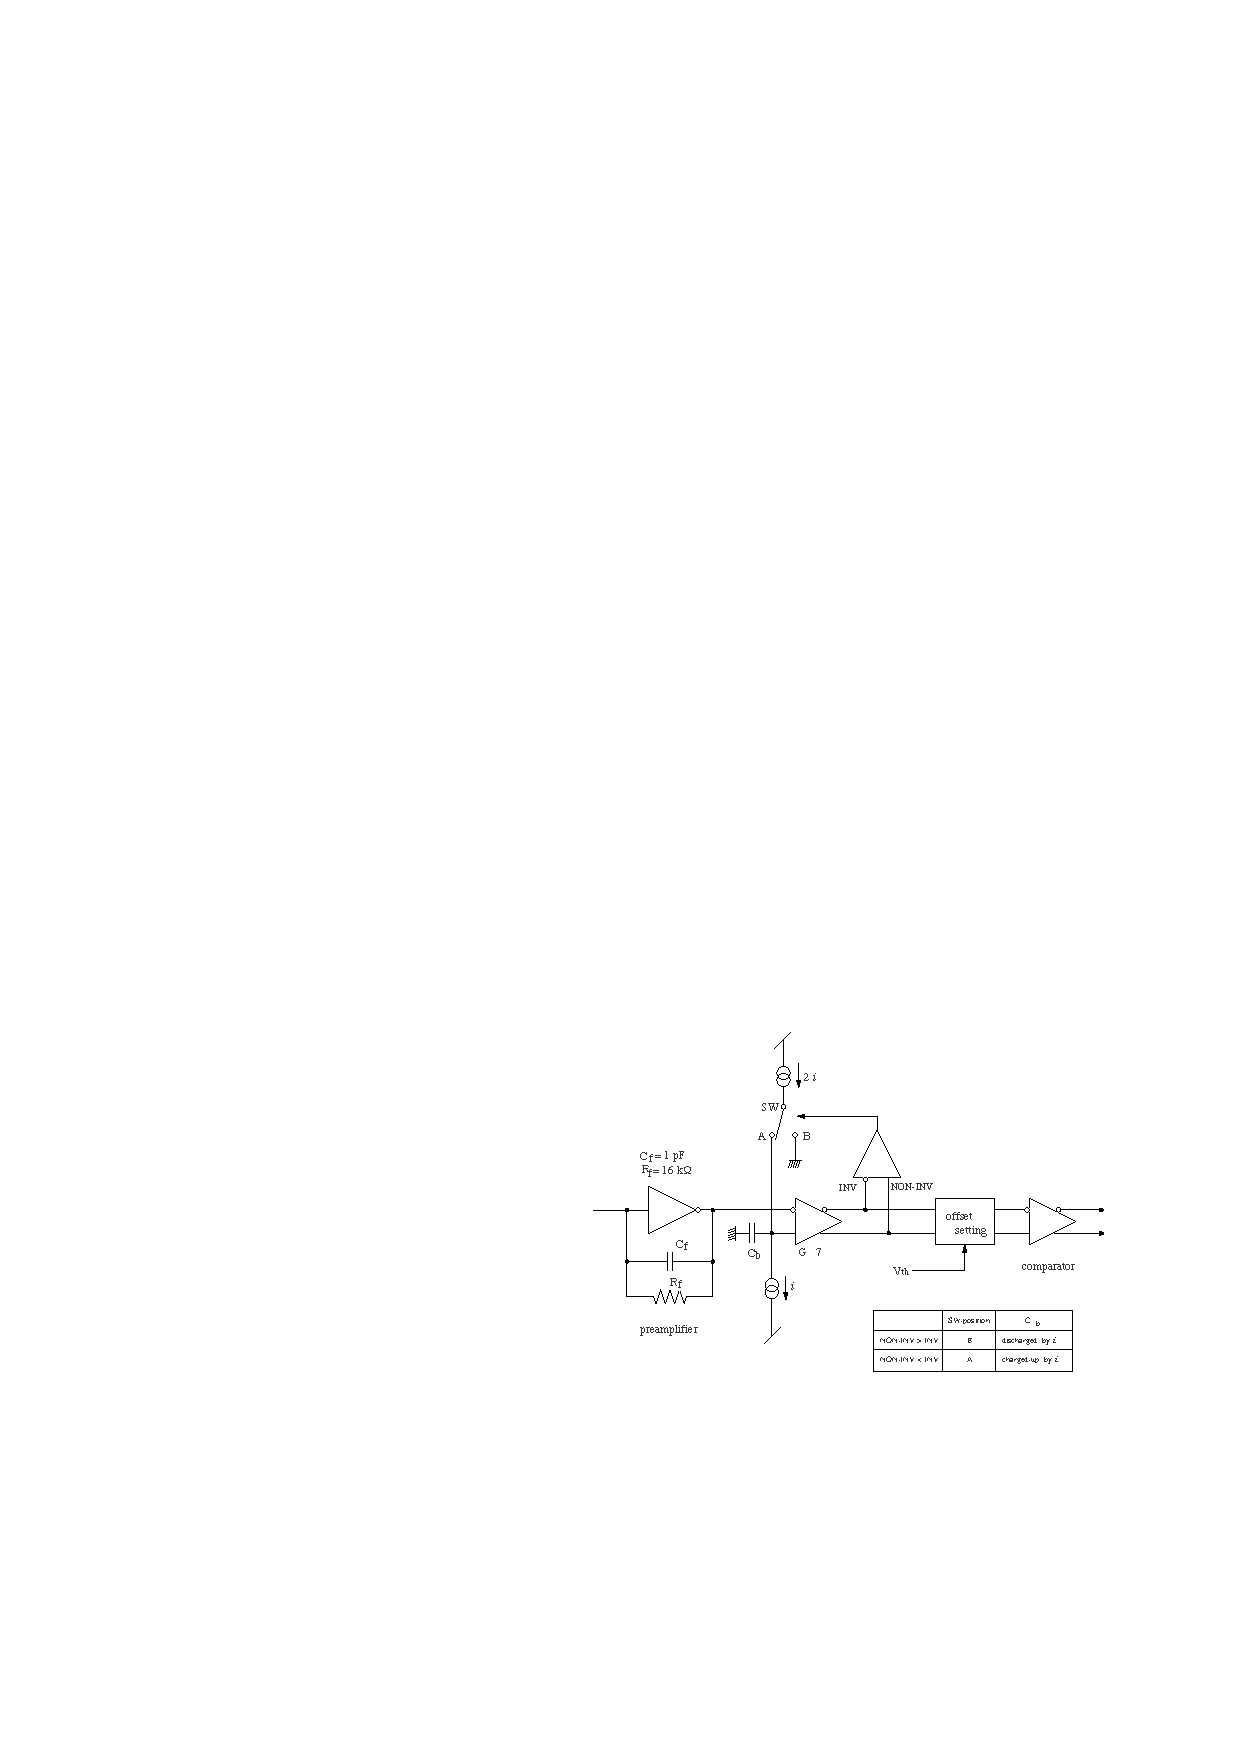
\includegraphics[height=5cm]{fig/Intro/TGC_ASDcircuite.pdf}
    \subcaption{ASDチップの回路ブロック図}
    \end{minipage}%
    \caption[ASDの概要]{ASDの概要\cite{ASD}}
    \label{TGC_ASD}
    \end{figure}

        \subsection*{Primary ProceSsor board (PS board)}
    ASDボードからのヒット信号は、次にPS boardに送られる。PS boardはPP ASICとXilinx 社製のKintex-7 FPGAという二つの集積回路を搭載している。PP ASICは各ASDからの入力信号の到着時間を揃え、その信号がどの陽子バンチ衝突に由来するかを識別する (BCID)。PS board FPGAはBCIDされたヒット信号を高速光シリアル通信に乗せてSLへ転送する。図\ref{TGC_PSB}にPS boardの最終試作機の写真とブロック図を示す。PS boardには8つのPPASICが搭載され、そのうち4つはメザニンカード上に乗せられる。1つのPP ASICは2台のASDと接続され、合計で32チャンネルの信号を処理する。PS board FPGAは8つのPP ASICからの信号をまとめ上げ、合計256チャンネル分のヒットデータをヒットの有無に関わらずSLに送る。
    PS boardはボード上にDAC  (Degital Analog Converter) 、ADC  (Analog Degital Converter) 、クロックジッタークリーナー、QSPIフラッシュメモリーなどの素子を搭載している。DACはASD ASICのコンパレーターにアナログの閾値電圧を供給するための素子であり、PS board FPGAから閾値電圧の大きさを設定することができる。ADCはDACから供給される閾値電圧をモニターする。クロックジッタークリーナーは、PS baord FPGAがシリアルデータから再構成したLHCバンチ衝突クロックのジッターを低減するために使用される。QSPI フラッシュメモリーは不揮発性のメモリーであり、ボードの電源が落とされた場合でも書き込まれた値を保持しておくことができる。これを利用してPS board FPGAのファームウェアやボードごとに定義されるPP ASICの遅延値などのパラメーターを保存する役割を果たす。
    またインターフェイスとして、電気信号を光信号に変換して光通信を行うSFP+モジュール、Cat-6ケーブルのコネクターであるRJ45を有しており、それぞれSLとJATHubに接続される。システム全体で1434枚のPS boardが設置される。

    以下にPP ASICとPS board FPGAの役割を詳しく説明する。

    \begin{figure}
    \begin{minipage}[b]{.5\linewidth}
    \centering
    \includegraphics[height=8cm]{fig/Intro/TGC_PSB.pdf}
    \subcaption{PS boardの写真}
    \end{minipage}%
    \begin{minipage}[b]{.5\linewidth}
    \centering
    \includegraphics[height=8cm]{fig/Intro/TGC_PSBblock.pdf}
    \subcaption{PS boardのブロック図}
    \end{minipage}%
    \caption[PS boardの概要]{PS boardの概要}
    \label{TGC_PSB}
    \end{figure}

    \subsubsection*{Patch-Panel ASIC (PP ASIC)}


    \begin{figure} 
    \centering
    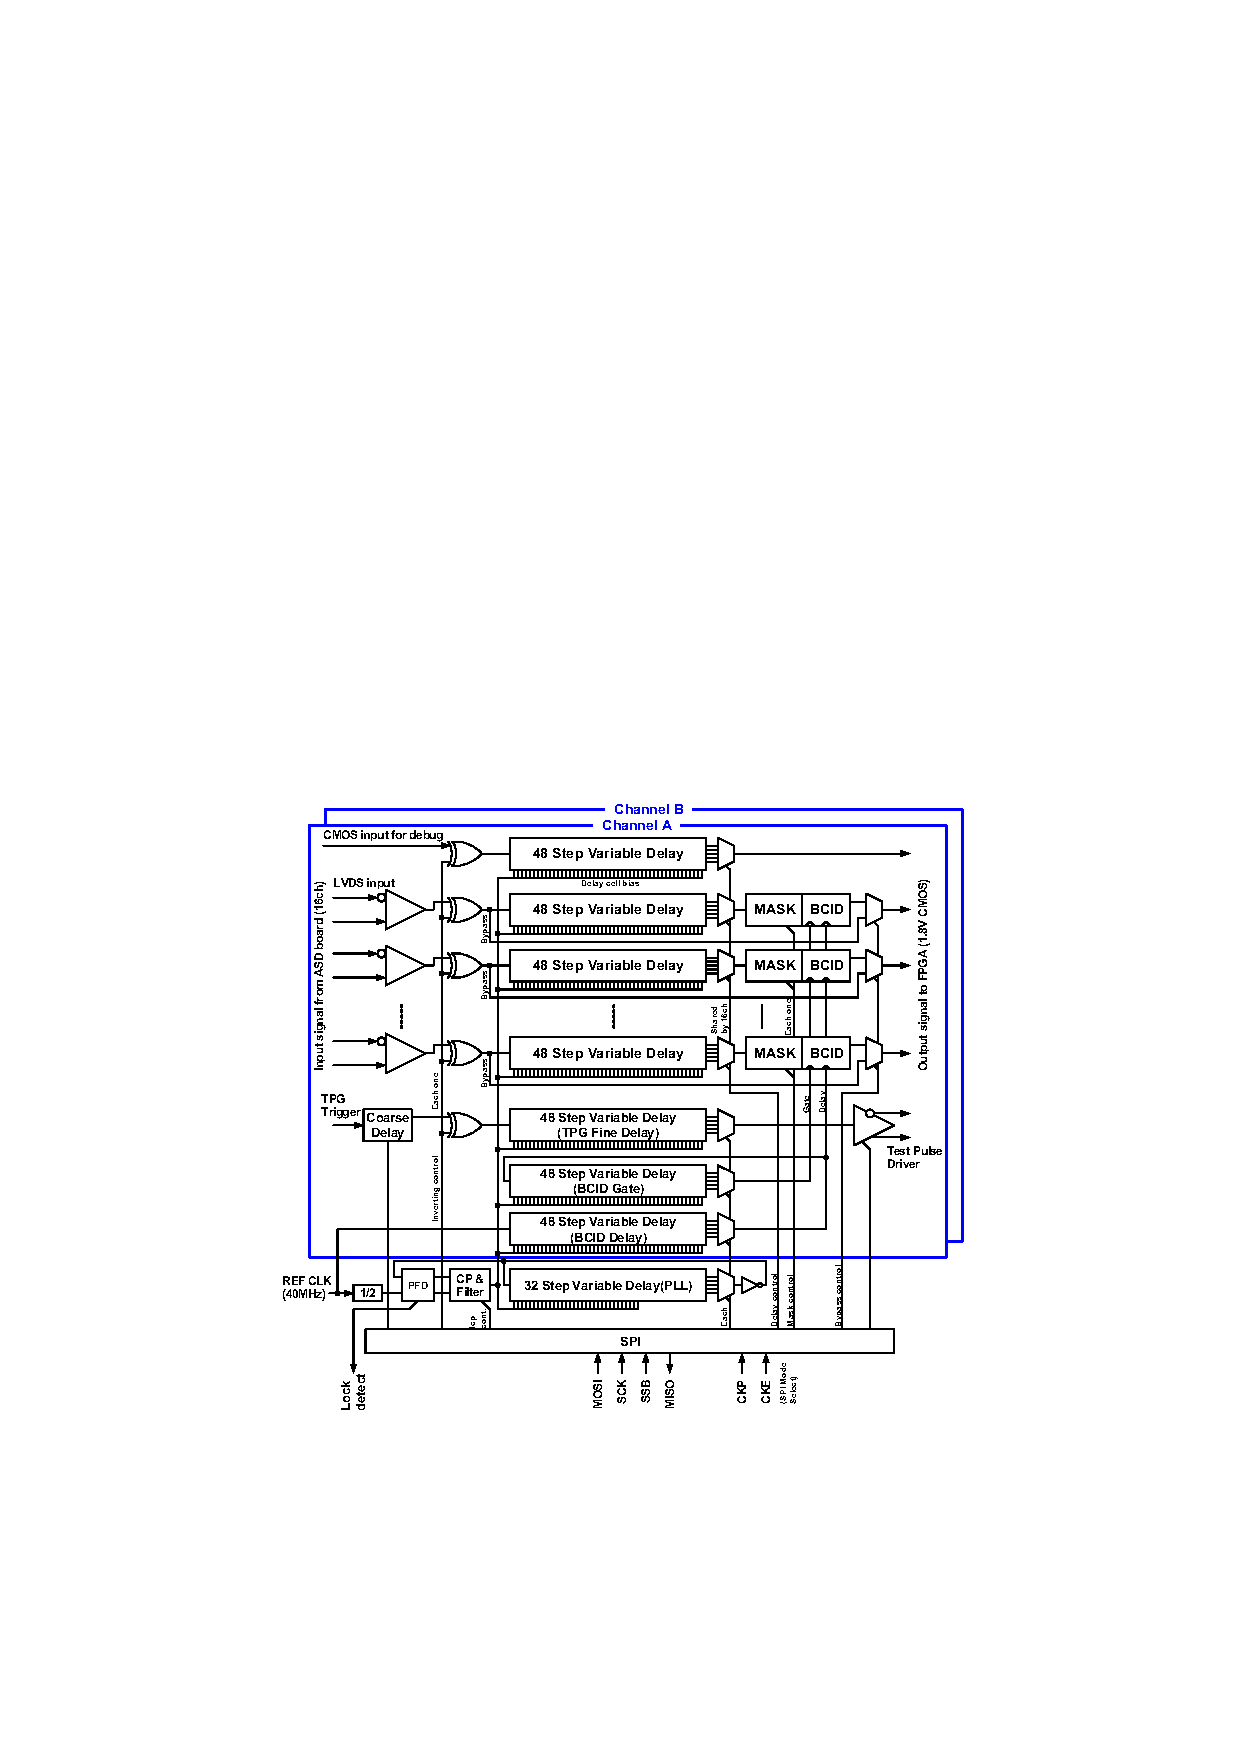
\includegraphics[width=16cm]{fig/Intro/TGC_PPASIC.pdf}
    \caption[PP ASIC回路のブロック図]{PP ASIC回路のブロック図\cite{PPASIC}}
    \label{TGC_PPASIC}
    \end{figure}

    図\ref{TGC_PPASIC}にPP ASICのブロック図を示す。PP ASICは主に可変遅延回路と陽子バンチ識別回路で構成される。PP ASICが受け取るLVDS信号の入力時間には、チャンネルごとに最大26 ns程度のばらつきが存在する。これは、チャンネルごとにミューオンの衝突点から検出器までの飛行時間  (Time-of-Flight) やASDからPP ASICまでのLVDSケーブルの長さが異なるからである。さらに、TGCの同じチャンネル内でもイベントごとに信号の到着時間が20 $\sim$ 30 ns程度変動する (\ref{TGC_fructuation})。これはミューオンの入射位置によって、チェンバー内で電荷が検出される位置からASDまでの距離や、電荷のドリフト時間が変わるからである。

    \begin{figure} 
    \centering
    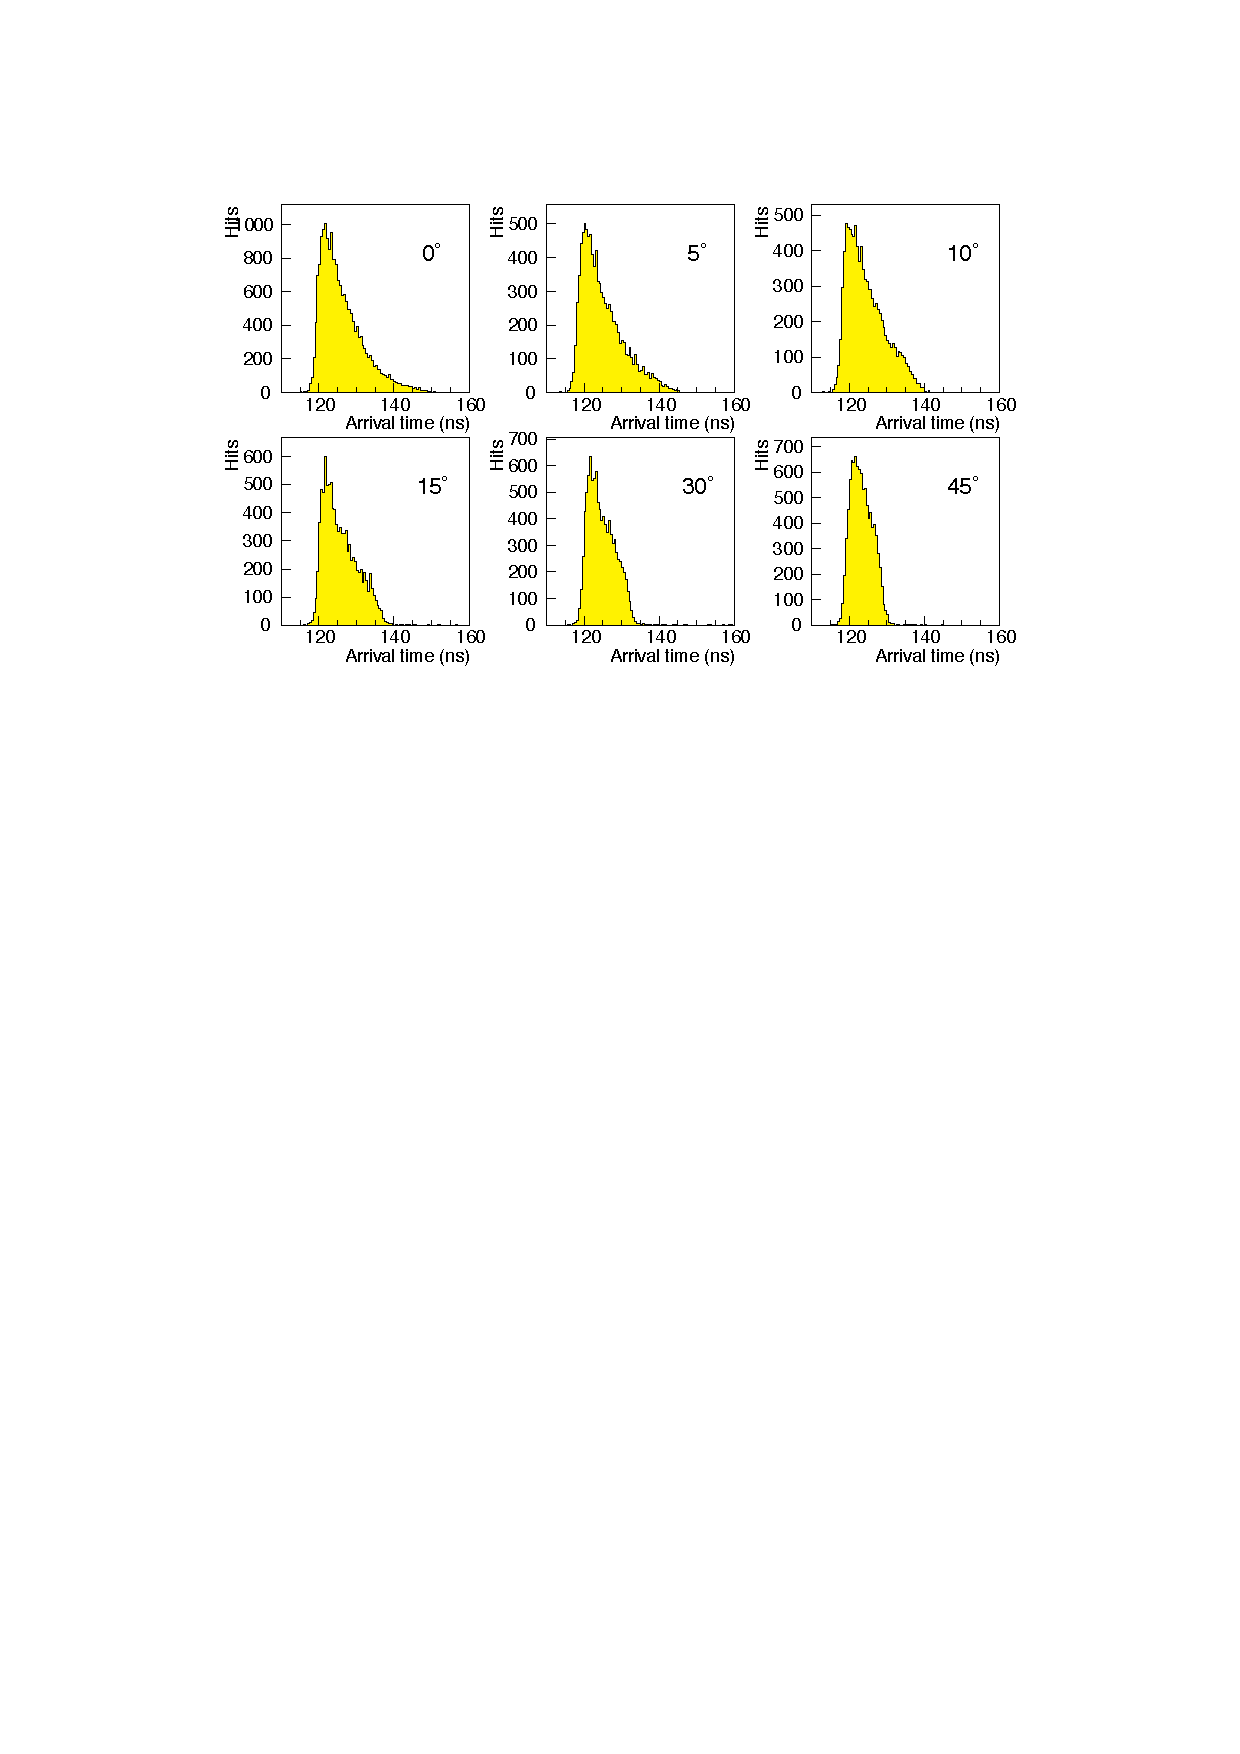
\includegraphics[width=16cm]{fig/Intro/TGC_fructuation.pdf}
    \caption[fructuation]{ミューオンがTGC検出器に入射してから、ASDに信号が到着するまでの時間分布\cite{TGC_fructuation}。時間分布はミューオンが入射する角度に依存して、20 $\sim$ 30 nsの幅を持つ。}
    \label{TGC_fructuation}
    \end{figure}

    このばらつきを揃えるために、各ASDごとに固有の遅延をかけるのが可変遅延回路である。可変遅延回路は1 ns以下の刻み幅で、最大45 nsの遅延をかけることができる。PP ASICに一番遅く到着するASDからの信号の立ち上がりと他のASDからの信号の立ち上がりを合わせる形で、遅延パラメーターが決められる。この遅延パラメーターはPS boardのFGPAから設定することができる。

    可変遅延回路でタイミングが揃えられた後、信号は陽子バンチ識別回路に送られる。陽子バンチ識別回路は、PP ASICに入射するデジタル信号の立ち上がりを検出し、その信号がどの陽子バンチ衝突に由来するのか識別する。陽子バンチ回路の概念図を図\ref{TGC_BCID}に示す。前述の通り、同じチャンネル内であってもヒット信号の到着時間はイベント毎に20 $\sim$ 30 ns程度の幅を持ち、この時間幅のうちに来るヒット信号には同じBCIDを付与する必要がある。そのため、同じBCIDを付与する時間幅 (有効ゲート幅) をASDごとに設定できるようになっており、信号到着時間幅が25 nsを超える場合に対応するため、有効ゲート幅は25 ns以上に設定できるようになっている。その場合、2つの有効ゲートが重なる時間が存在するが、このタイミングに入射した信号には2バンチ分の信号が出力される。有効ゲート幅もPS boardのFPGAから設定することができる。

    \begin{figure} 
    \centering
    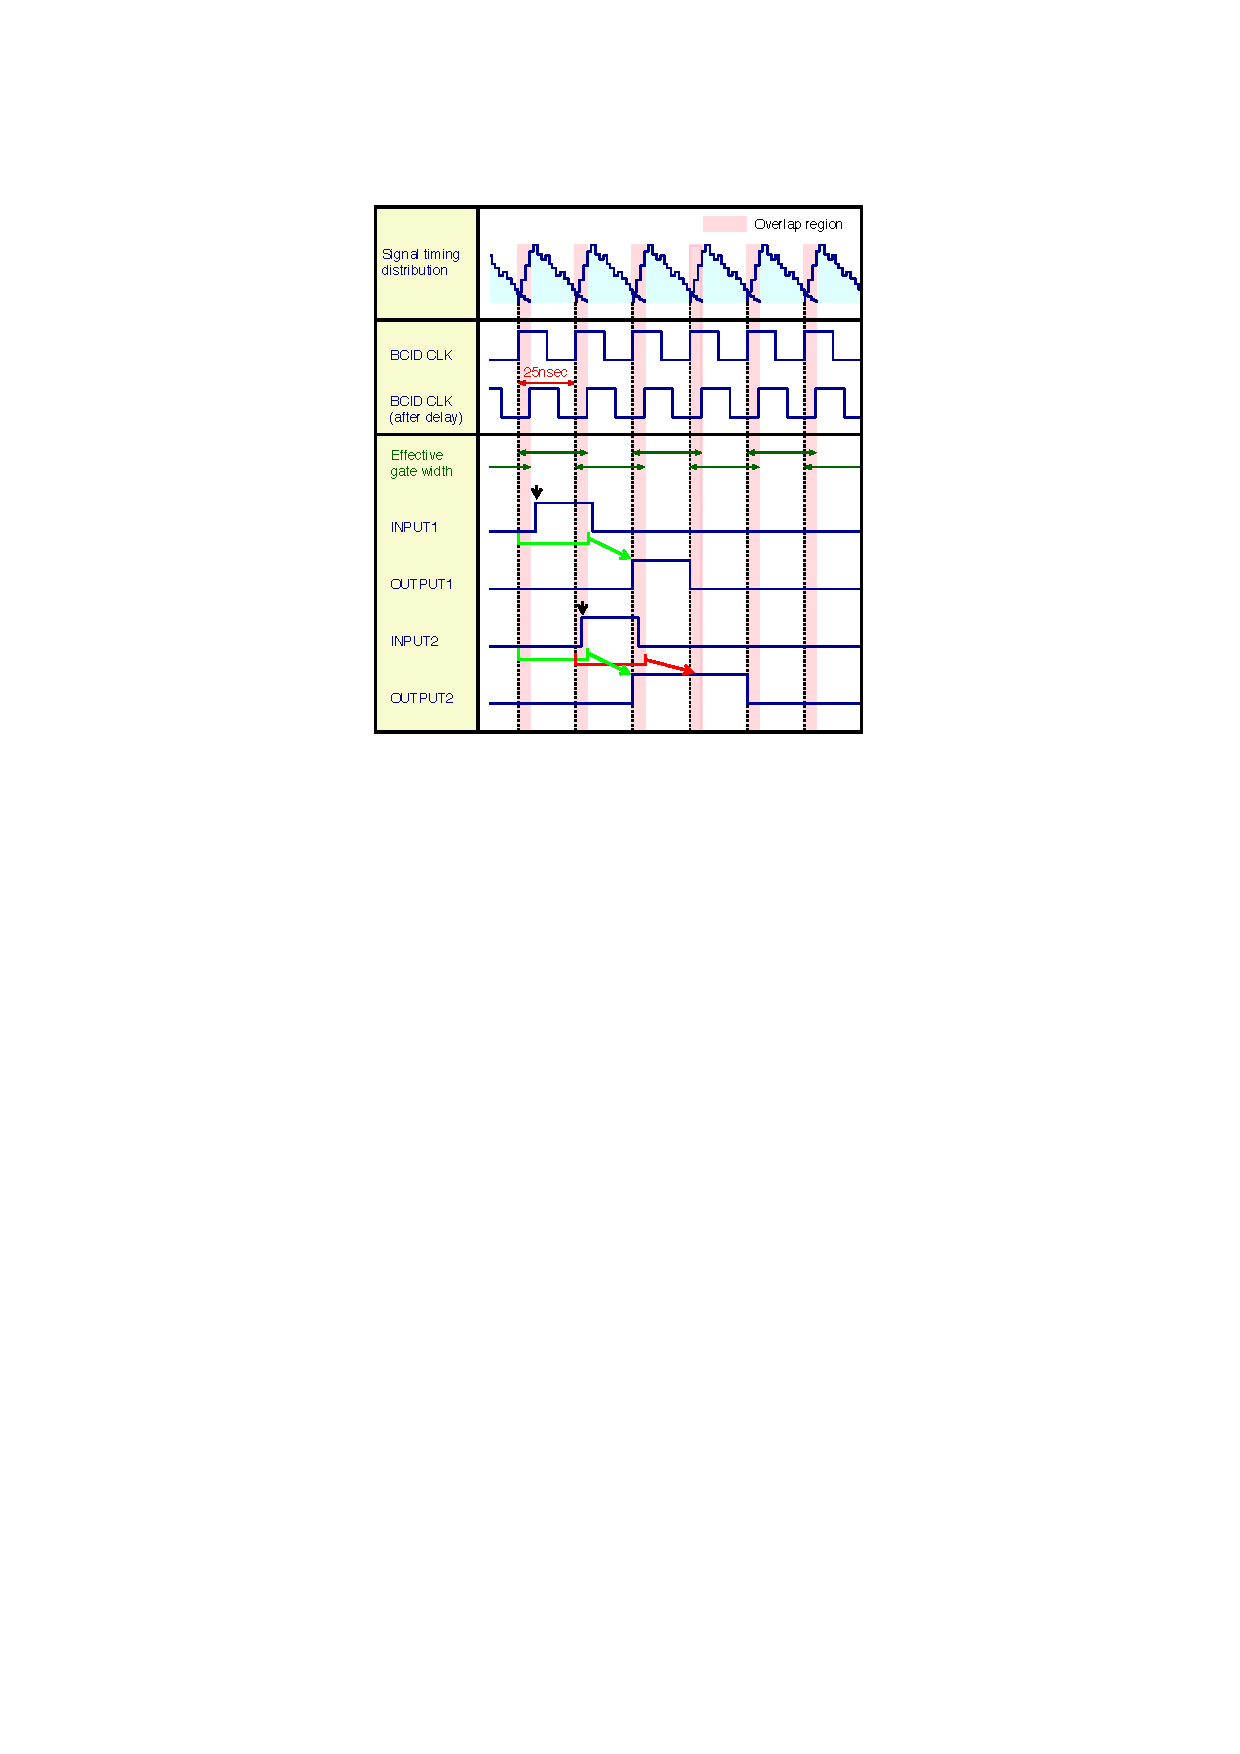
\includegraphics[width=16cm]{fig/Intro/TGC_BCID.pdf}
    \caption[陽子バンチ識別回路のタイミングチャート]{陽子バンチ識別回路のタイミングチャート\cite{mt_takemoto}}
    \label{TGC_BCID}
    \end{figure}

    \subsubsection*{PS board FPGA}

    PS board FPGAはSLへのヒットデータ転送に加えて、PS board上の各素子の制御/監視およびLHCバンチ交差クロックの再構成も担当する。
    8つのPP ASICでLHCバンチ交差クロックと同期された256チャンネルのヒット信号は、PS board FPGAで集められ、光ファイバーを通じてSLに転送される。
    PS boardからSLに送られるデータフォーマットを図\ref{TGC_PSBuplink}に示す。256チャンネルのヒットデータに加え、64 bitのヘッダーが付与され合計320 bitのデータが25 nsおきに送信される。320 bitのデータは2本の光ファイバーに分けられ、32 bitごとにワードとしてまとめられて送信される。ここでワード0ではヘッダーが、ワード1 $\sim$ 4にはヒットデータが詰められる。データ転送には高速シリアル通信に対応したGTXトランシーバーを用いる。ここでは8b10bコーディングが用いられ、FPGA内のパラレルデータをシリアルデータに変換し、高速シリアル通信を実現をする。そのため、1本の光ファイバーのラインレートは$160 \, \mathrm{bit} \times 10/8 \times 40 \mathrm{\,MHz} = 8 \,\mathrm{Gbps}$となる。

    \begin{figure} 
    \centering
    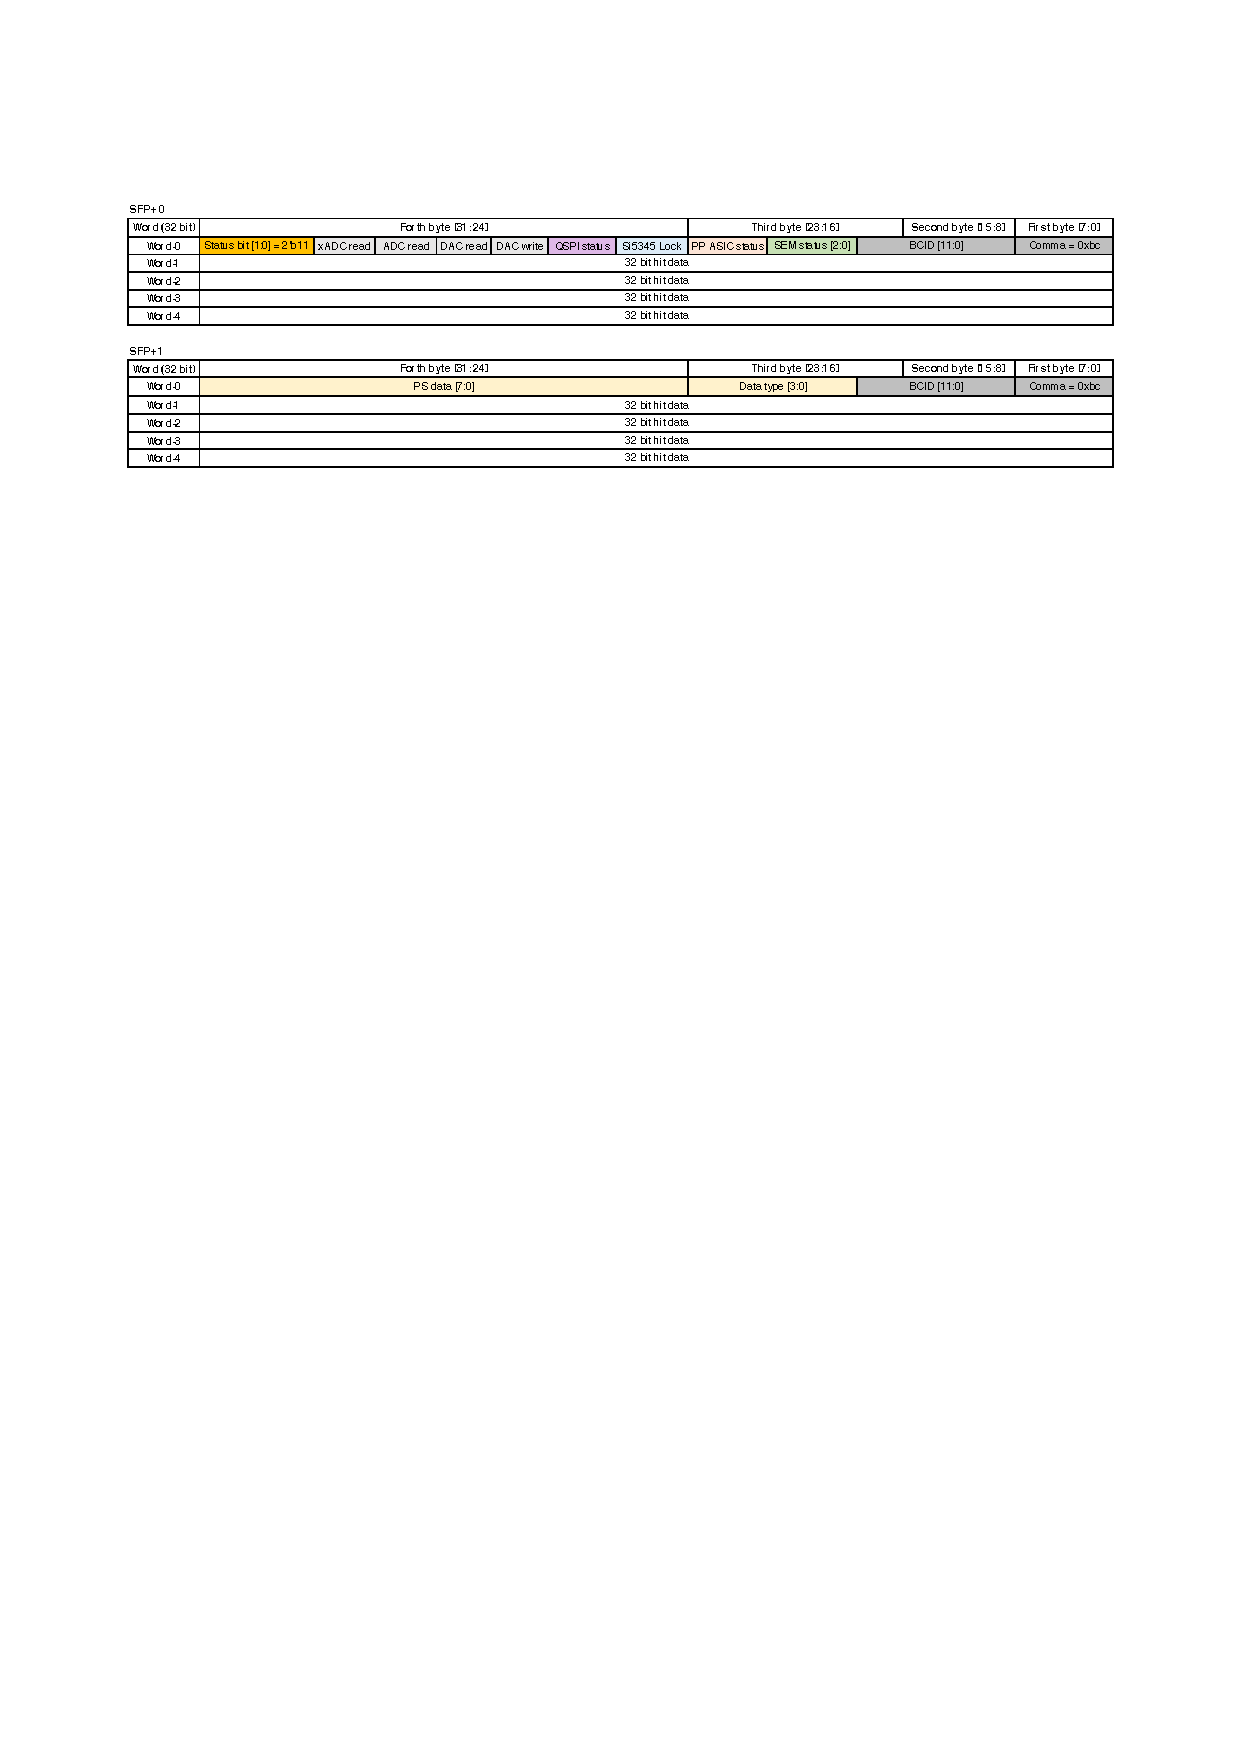
\includegraphics[width=16cm]{fig/Intro/TGC_PSBuplink.pdf}
    \caption[PS boardからSLへ送るデータフォーマット]{PS boardからSLへ送るデータフォーマット\cite{mt_aoki}}
    \label{TGC_PSBuplink}
    \end{figure}

    PS board FGPAはSLからコントロール用の信号を1本の光ファイバーを通じて受け取る。SLからPS boardに送られるデータフォーマットを図\ref{TGC_PSBdownlink}に示す。SLはワード2と3で定義されたAddress、Data、Commandを利用してPS board FPGA内のレジスタを操作する。また、PS board FPGAとQSPIフラッシュメモリーはSPIバスで接続されており、SLがFPGAを経由してSPIバスをビットバンギングすることで、QSPIフラッシュメモリーにデータを書き込むことができる。このパスを利用して、PP ASICの遅延パラメーターや有効ゲート幅、ASDに供給する閾値電圧など、各PS board毎に異な値を設定する必要がある制御用パラメーターをQSPI フラッシュメモリー上に保存することができる。
    そして、PS board FPGAはQSPIフラッシュメモリーに書き込まれた制御用パラメーターを自動で読み取り、PP ASIC、ASDに分配する。これを自立型制御機構と呼ぶ。この機構により、1434枚のPS boardには同じファームウェア\footnote{正確にはPS boardからSLに送るデータフォーマットに3種類のバラエティが必要であるため、3種類のファームウェアを使い分けることになる。}を書き込んだ上で、ボード毎に必要な設定は自動で行うという、次世代的な制御モデルを実現している。
    PS board FPGA にはPS board上の素子の状態を監視するための機構も備わっており、DACに分配した設定値、ADC、xADC\footnote{Xilinx Analog-Digital Converter、FPGA内部の温度、電源電圧、外部からのアナログ信号を監視するためのモジュール。PS boardに供給される3.3 VD  (デジタル) 、+ 3 VA  (アナログ) 、-3 VAをモニターする}のモニター値、GTXトランシーバーのロック信号を定期的に読み出し、SLに送信する。これを自立型監視機構と呼ぶ。これによりコントロールマスターのSLはフロントエンドのPS boardの状態を常に把握し、異常が生じた際には瞬時に対応することができる。

    \begin{figure} 
        \centering
        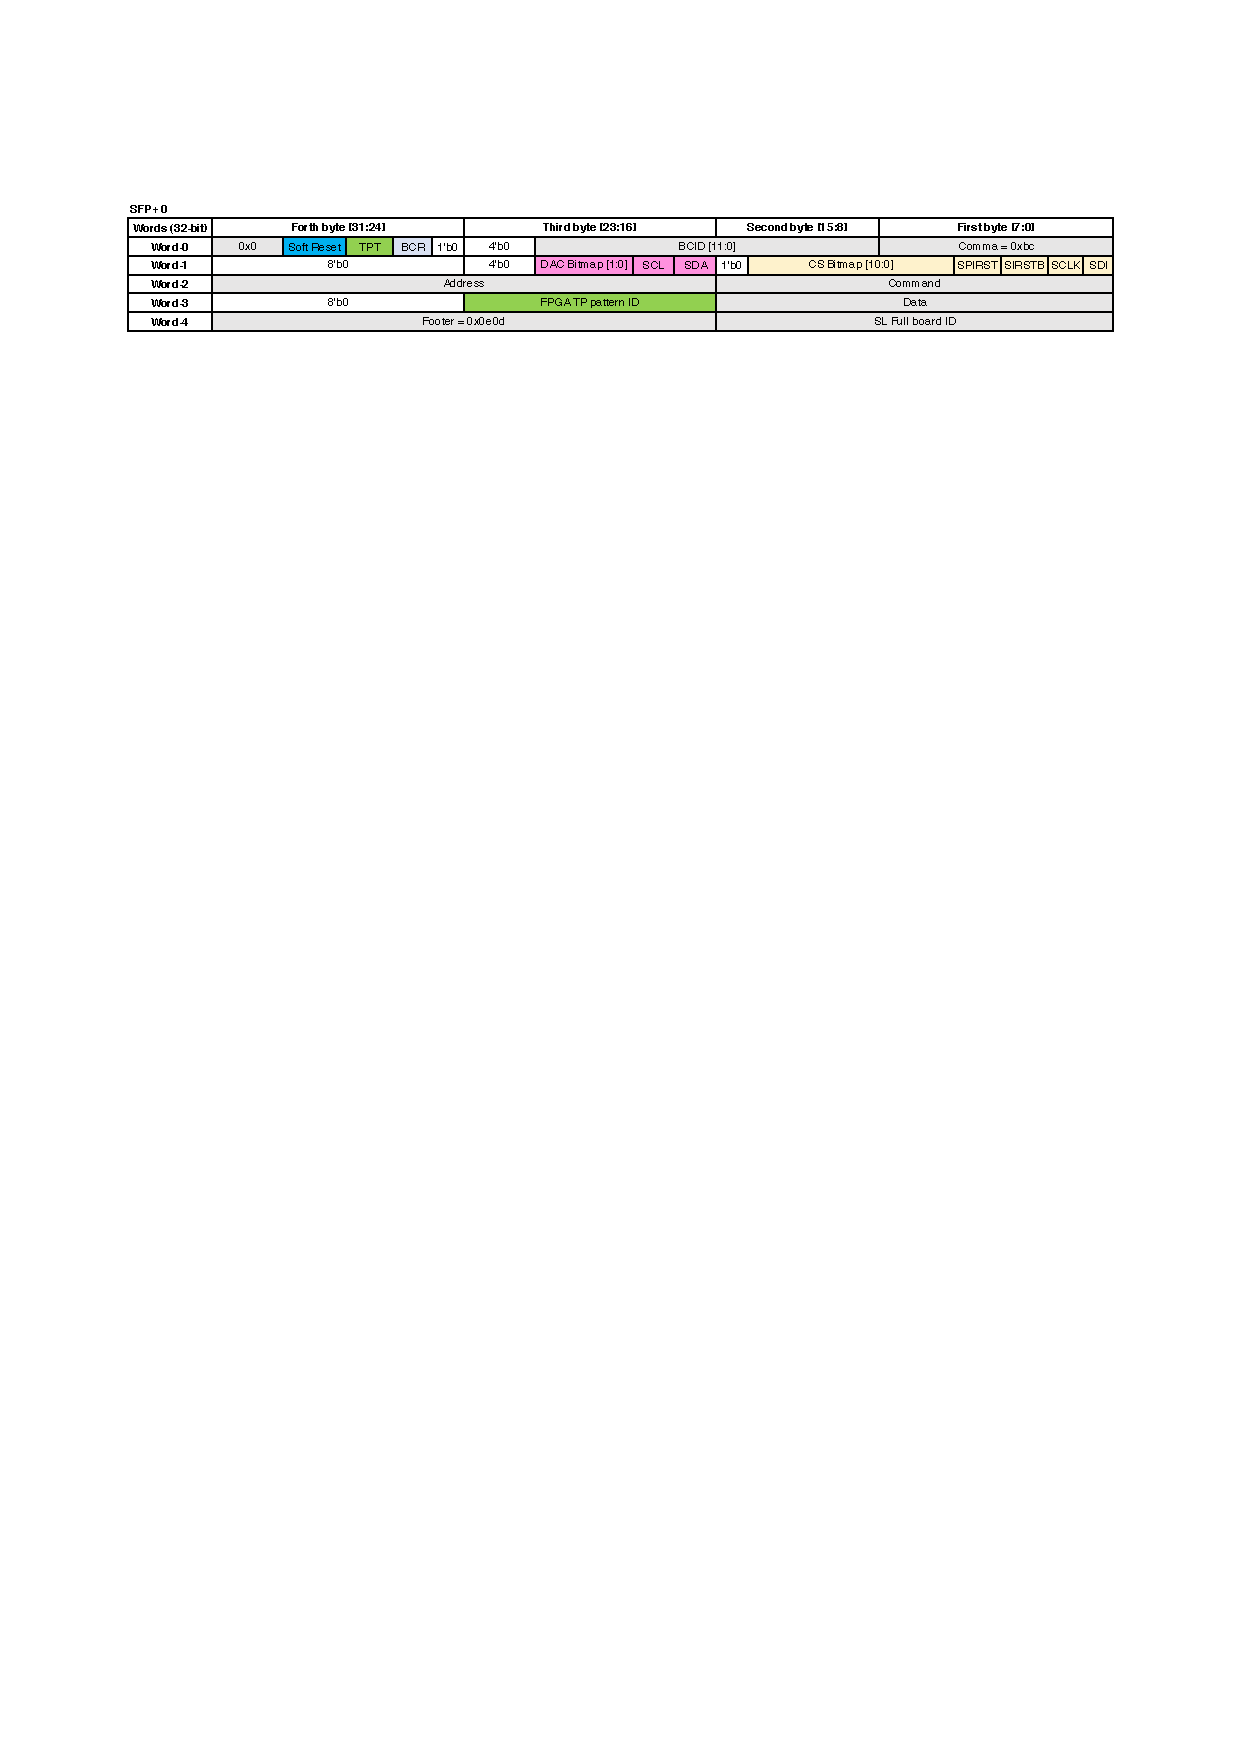
\includegraphics[width=16cm]{fig/Intro/TGC_PSBdownlink.pdf}
        \caption[SLからPS boardへ送るコントロールデータのフォーマット]{SLからPS boardへ送るコントロールデータのフォーマット\cite{mt_aoki}}
        \label{TGC_PSBdownlink}
    \end{figure}
    
    TTC信号もこのコントロール線に乗せられてPS boardに分配される。PS boardのGTXトランシーバーは、ワード0で定義されるComma ワードを使用して、シリアルデータからLHCバンチ交差クロックを再構成する。PS boardで再構成されたLHCバンチ交差クロックは適切な遅延が加えられた後、ジッタークリーナーを経由してFPGA、GTXトランシーバー、PP ASICへ分配される。    

    さらに、PS boardは放射線損傷に対する堅牢性を実現するシステムを搭載している。PS boardは実験室に置かれるため、FPGAは電子回路上のメモリのビットが反転してしまうSingle Event Upset  (SEU) などの放射線損傷を受ける可能性がある。先行研究\cite{PSB_SEU}によると、1つのPS board FPGAでは3時間に一回程度SEUが発生することが予想される。FPGAには修復可能なSEU  (1ビットエラーおよび隣接する2ビットエラー)を自動的に修復するSoft Error Mitigation Controller  (SEM) が実装されている。また修復不可能なSEU  (隣接しない2ビットエラーおよび3ビット以上のエラー) が生じた際には、PS boardの制御を担当するフロントエンドエレクトロニクスであるJATHubに対して救難信号を送り、JATHubからFPGAの再コンフィギュレーション用の信号を送ってもらうことでこれに対処する。これらの放射線損傷に対する堅牢なシステムを実現することで、データ取得時のデッドタイムを最小限に抑えることができる。

        \subsection*{JTAG AssisTance Hub (JATHub)}
    JATHubはデータパスとは独立した、PS board制御用の回路である。概要を図\ref{TGC_JATHub}に示す。JATHubはXilinx社製のZynq-7000 SoCをメインドライバーとして搭載する。Zynqはプロセッサー部分であるProcessing System  (PS) と、FPGA部分であるProgrammable Logic  (PL) で構成されている。PSにLinuxなどのカーネルを立ち上げ、C言語などで記述したアプリケーションを実行することでFPGAを操作することができる、高い自由度と拡張性を兼ね備えたデバイスである。
    JATHubはインターフェイスとして、PS boardとLVDS通信をするためのRJ45コネクターと、ATLAS回路室とのイーサーネット通信をするためのSFP+モジュールを搭載している。1枚のJATHubは最大で11枚のPS boardと接続可能であり、それぞれ2本のCat-6\footnote{Category-6 ケーブル。4対8線の動線で構成されており、4種類の差動信号線を束ねている。}ケーブルで接続される。一本のCat-6ケーブルはJTAGプロトコルでのビットバンギング用に定義されており、JTAG線と呼ぶ。FPGAはStatic Random Access Memory  (SRAM) にファームウェアを書き込むことにより、内部の論理回路を何度でも書き直すことができる。しかし、一般にファームウェアを書くには、書き込み用アプリケーションが走るホストPCをFPGAの近くまで持っていき、JTAG4線用のCopperケーブルでホストPCとFPGAを接続させる必要がある。PS boardはTGC検出器上に設置されており、実質的にそのようなアクセスはできない。そこで遠隔からのファームウェア書き込みの中継点として、JATHubが機能する。回路室のネットワークからJATHubにアクセスし、PSでアプリケーションを走らせることで、遠隔でJTAG線をドライブすることができる。また、SRAMは揮発性のメモリであり、PS boardの電源を入れ直すたびにファームウェアを書き直す必要があるが、PS boardではQSPIフラッシュメモリーにファームウェアを保存することで、電源を入れ直すと自動で電子回路を構成することができるようになっている。
    もう一本のCat-6ケーブルはPS boardの放射線損傷に対する回復、およびLHCバンチ交差クロックの再構成に利用され、Recovery/Monitor線と呼ぶ。図\ref{JATHubsem}にJATHubのRecovery/Monitorパスの概要を示す。PS board FPGAで自己修復不可能なSEUが生じた場合、RcvB線を通じて救難信号が出される。JATHubはこれを受けるとPS boardにFPGA再コンフィギュレーション用の信号をPROGB線を通じて送信する。この一連の手続きをリカバリー手続きと呼ぶ。MON線はPS boardが再構成したLHCバンチ交差クロックをJATHubに送信するために利用される。JATHubは接続される11台のPS boardで再構成されたクロックの位相をモニターし、その位相差を測定する。

    \begin{figure} 
        \centering
        \includegraphics[width=16cm]{fig/Intro/TGC_JATHub.pdf}
        \caption[JATHubの概要]{JATHubの概要}
        \label{TGC_JATHub}
    \end{figure}

    \begin{figure} 
    \centering
    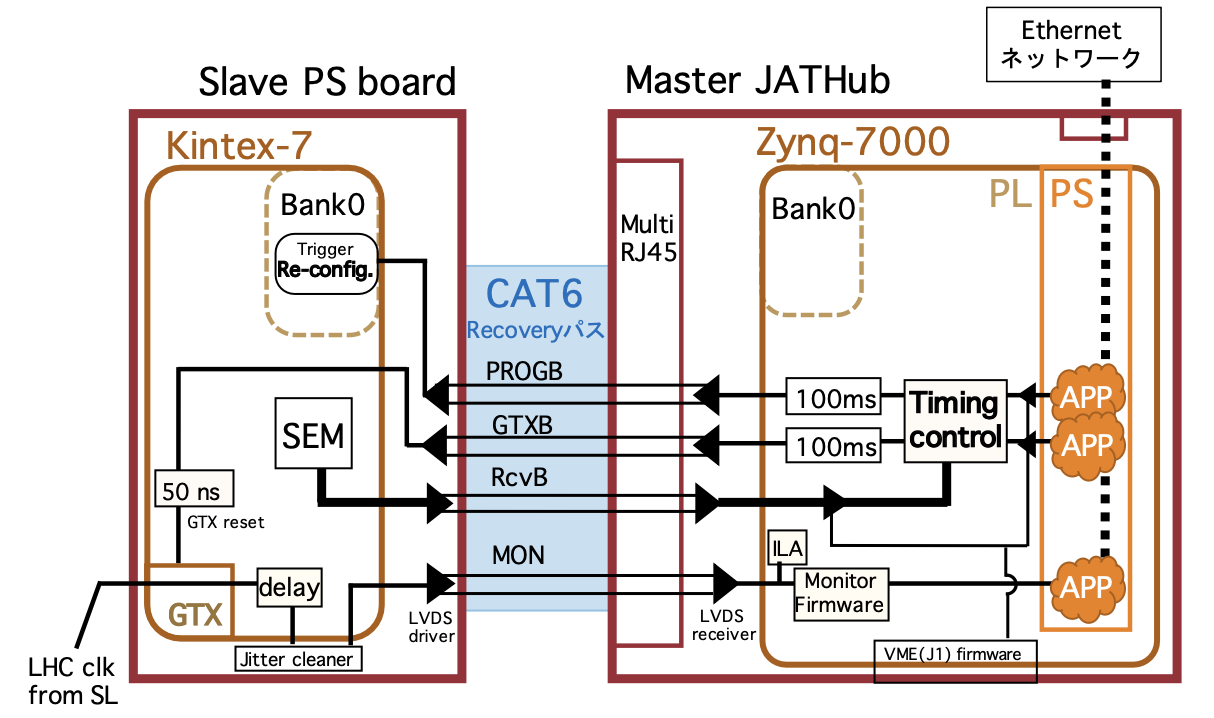
\includegraphics[width=16cm]{fig/QAQC/JATHubsem.png}
    \caption[JATHub によるリカバリー手続きの概要]{JATHub によるリカバリー手続きの概要\cite{mt_atanaka}。PS board に自己修復不可能な SEU 事象が発生した場合、RcvB線を通じてJATHubに救難信号が発出される。これを受信したJATHubはPROBG線をアサートすることでPS board FPGAの再コンフィギュレーションを行う。}
    \label{JATHubsem}
    \end{figure}

        \subsection*{Sector Logic  (SL) }
PS board FPGAでまとめられた256チャンネル分のヒットデータはSLに集められる。SLはVirtex UltraScale+ FPGAという大規模FPGAとZynq UltraScale+ MPSoCという2つの集積回路を搭載している。Virtex UltraScale+ FPGAのデバイスはSL FPGAと呼ばれ、PS boardから受信したヒットデータを用いてトリガー演算を行う。また、SL FPGAはCTPからL0Aが発行されるまでのデータバッファリングおよび後段への読み出しも担当する。Zynq UltraScale+ MPSoCはVirtex UltraScale+ FPGAやPS boardのコントロールマスターとして機能する。

\begin{figure} 
    \centering
    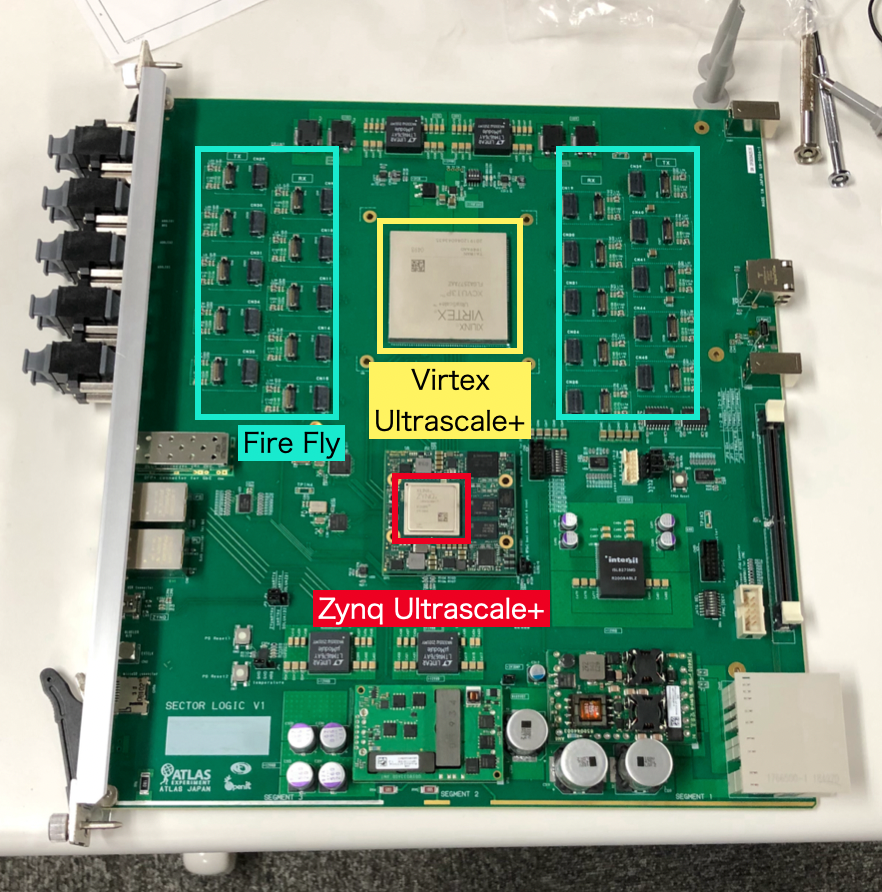
\includegraphics[width=16cm]{fig/Intro/TGC_SL.jpg}
    \caption[SL第一試作機の写真]{SL第一試作機の写真}
    \label{TGC_SL}
\end{figure}

SLの第一試作機の写真を図\ref{TGC_SL}に示す。
SLはAdvanced Telecommunications Computing Architecture (ATCA)規格のボードである。ユーザーはATCAクレートのShelf managerからCERNで開発されたIntelligent Platform Management Controller  (IPMC) を介して、SLの電源や電圧のモニター、遠隔での電源操作を行うことができる。SLは外部とのインターフェイスとして電気信号を光信号に変換するためのFireFlyを送信用に10個、受信用に10個搭載している。それぞれが12リンクを束ねるため、送受信120リンクの光通信が可能である。LANケーブルのインターフェイスであるRJ45コネクターも搭載しており、ethernetを介したネットワーク通信も可能である。

1枚のSLはTGCの1/24セクターからの信号処理を担当し、合計31台のPS boardと接続する (BW用に29 枚、EI用に2 枚)。AsideとCsideを合わせて、合計で48枚のSLが設置される。以下にそれぞれの集積回路の機能の詳細を述べる。

    \subsubsection{SL FPGA}
SL FPGAに実装するファームウェアの概要を図\ref{SL_FW_overview}に示す。ファームウェアは大別してトリガー回路、読み出し回路、コントロールパスに分けられる。PS boardから光リンクを経由して送られるヒット情報は、トリガー回路および読み出し回路に入れられる。

\begin{figure} 
\centering
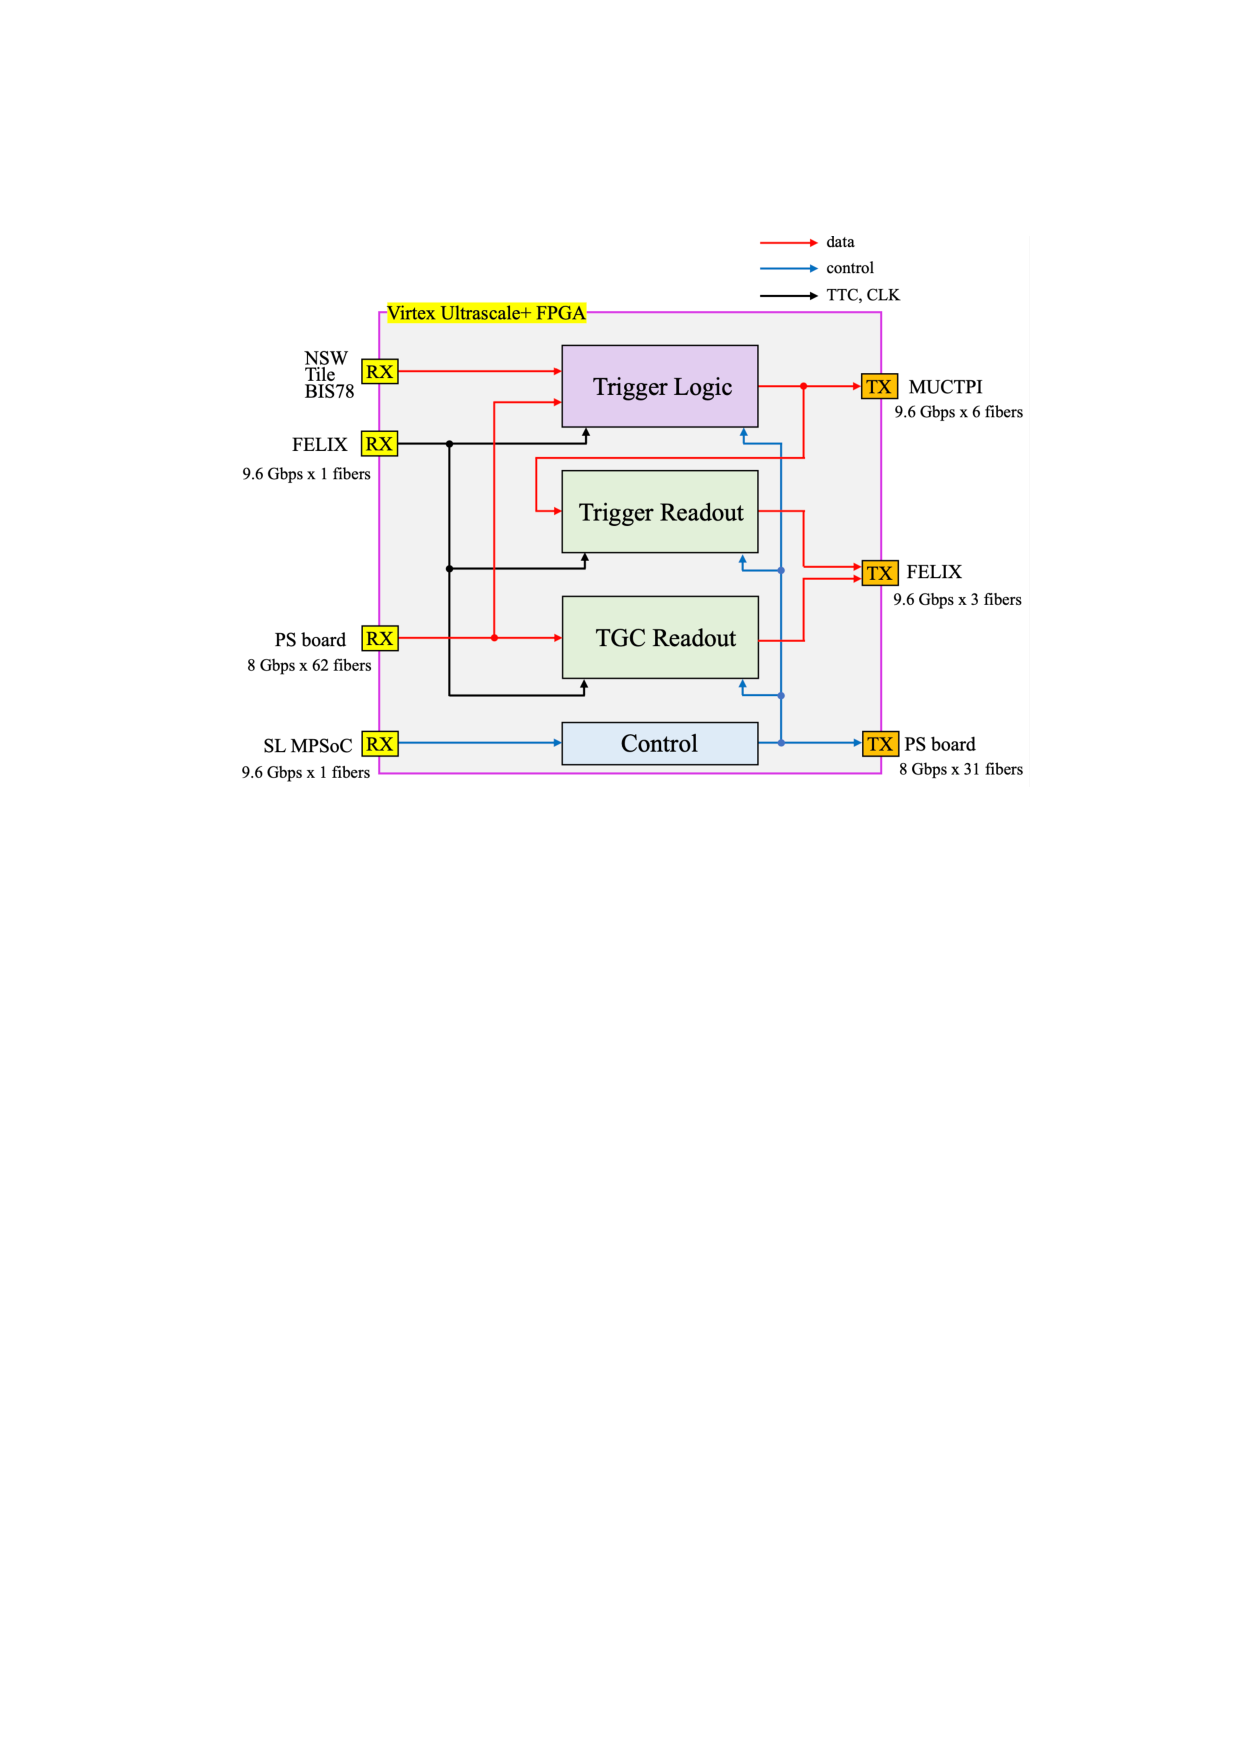
\includegraphics[width=16cm]{fig/Intro/SL_FW_overview.pdf}
\caption[SL FPGAに実装されるファームウェアの概要]{SL FPGAに実装されるファームウェアの概要\cite{mt_mishima}}
\label{SL_FW_overview}
\end{figure}

トリガー回路は、PS boardから送られるBW 7層分のヒットデータを用いて\pt 判定を行なった後、エンドキャップトロイド磁石より内側にあるNSW、RPC BIS78、TIleカロリメーターからの情報も用いて、より精度の高い\pt の概算を行う。
トリガー回路の出力は、L0 TriggerのためにMUCTPIへ転送される。またトリガーラインの正常動作を確かめるため、モニター用のデータがFELIXに転送される。
トリガー回路はこれまでにATLAS TGC JAPAN グループの共同研究として開発が進められてきた。本研究では開発されたモジュールの全体ファームウェアへのの統合および試験システムの開発を行った。これについては\ref{chap_TriggerIntegration}章、\ref{chap_TriggerTest}章で説明する。

読み出し回路は、PS board から送られてきたヒットデータとそのイベントに対応するトリガーデータをバッファーしておき、L0A が発行されたイベントのデータを選択的に後段へ転送する役割を担う。読み出されるデータにはゼロサプレスという圧縮処理が行われ、すべてのPS boardからのデータをイベントごとにパッキング  (Event Building) してから、FELIXに送信する。

コントロールパスは、SL FPGA内の設定やパラメーターの制御など、LHC バンチ交差クロックと同期する必要のないスローな制御を担当する。コントロールマスターのMPSoCからSL FPGA内のレジスタを操作することで、SLのトリガー・読み出しに関連するパラメーターの設定や、PS boardの制御を行う。

SL FPGAは4つのシリコンダイ (Super Logic Region, SLR) から構成される大規模FPGAである。図\ref{ISEE_abstract}に示すように、隣接するSLRはSuper Long Line (SLL) と呼ばれる専用のワイヤーで接続されていて、これを介して信号の送受信を行う。

\begin{figure} 
\centering
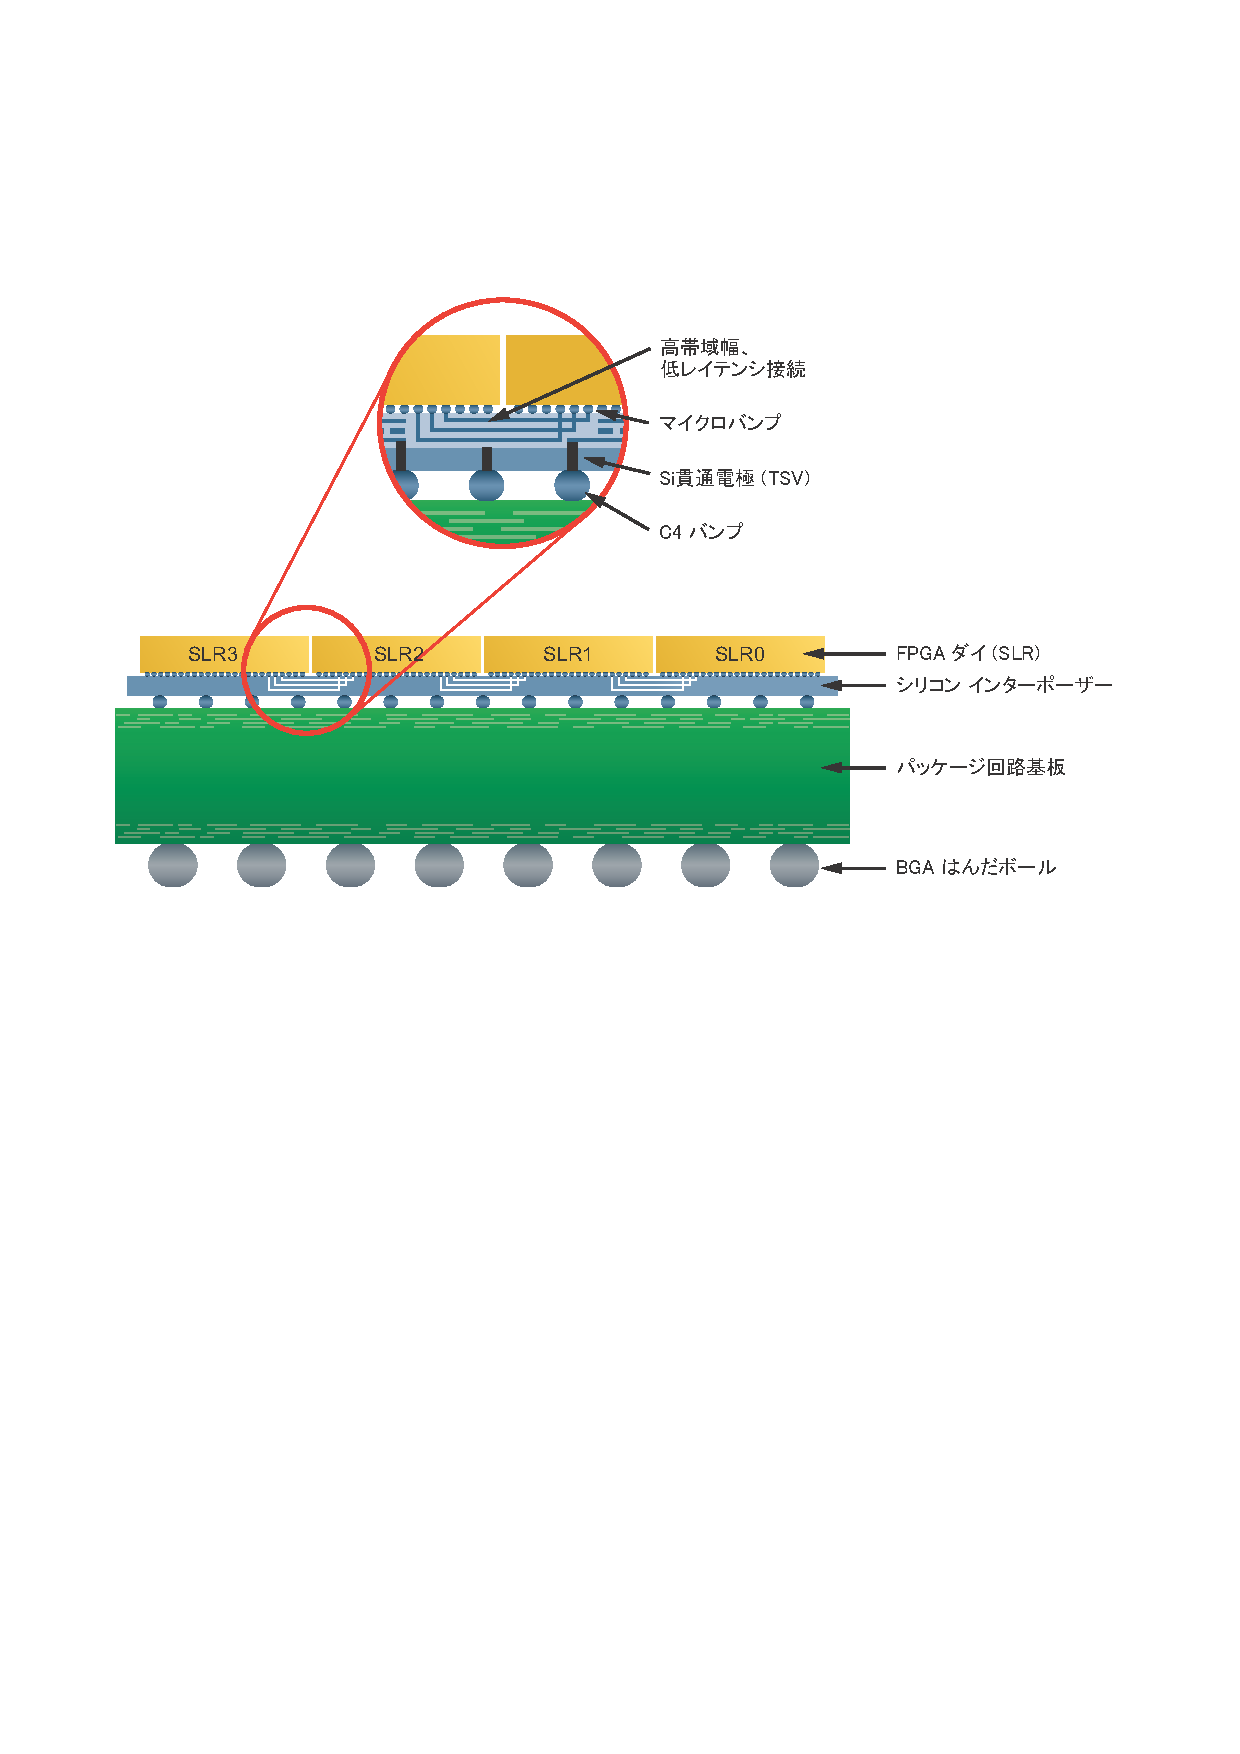
\includegraphics[width=16cm]{fig/Intro/ISEE_abstract.pdf}
\caption[SLRの概略図]{SLRの概略図}
\label{ISEE_abstract}
\end{figure}

ただ、SLLを介した信号の伝搬は通常よりも大きなレイテンシーがかかる。また、SLLの位置はSLR内で物理的に決まっているため、SLLが不要に多い設計ではタイミング制約を満たすのが厳しくなる。ファームウェア全体をタイミング制約やリソース使用量などの物理制約を満たして1枚のFPGAに実装しきるためには、どのSLRにI/Oや各ロジックを配置するか決めるフロアマッピングが重要となる。

図\ref{SL_floor}に設計されたSL FGPAのフロアマッピングを示す。PS boardからのヒット信号はSLR0・2・3で受信し、磁場内部の検出器からの信号はSLR1で受信する。そのため、TGCのヒット信号のみを用いるトリガーロジック ( TGC BW コインシデンス ) はそれぞれのSLRに配置し、データ量を削減した後、SLR1で磁場内部の検出器とのコインシデンスをとる。トリガーロジックはSLRごとにトリガーセクターを分けて配置しており、SLR0がエンドキャップ$\phi\,0$、SLR2がエンドキャップ$\phi\,1$、SLR3がフォワード領域を担当する。MUCTPIやMDTTPなどトリガー出力を送信するリンクはそのままSLR1に配置する。SLからFELIXにヒットデータを送信するリンクはSLR3に配置する。SLRを超える信号をできるだけ小さくするため、読み出し回路はZero Suppressなどのデータ圧縮作業はそれぞれのSLR内で行い、SLR3でイベントごとにパッキングして送信する。
MPSoCとSL FPGAのチップ間通信のためのリンクもSLR3に実装する。各SLRのレジスタ操作はSLR3を中継に行う。

\begin{figure} 
\centering
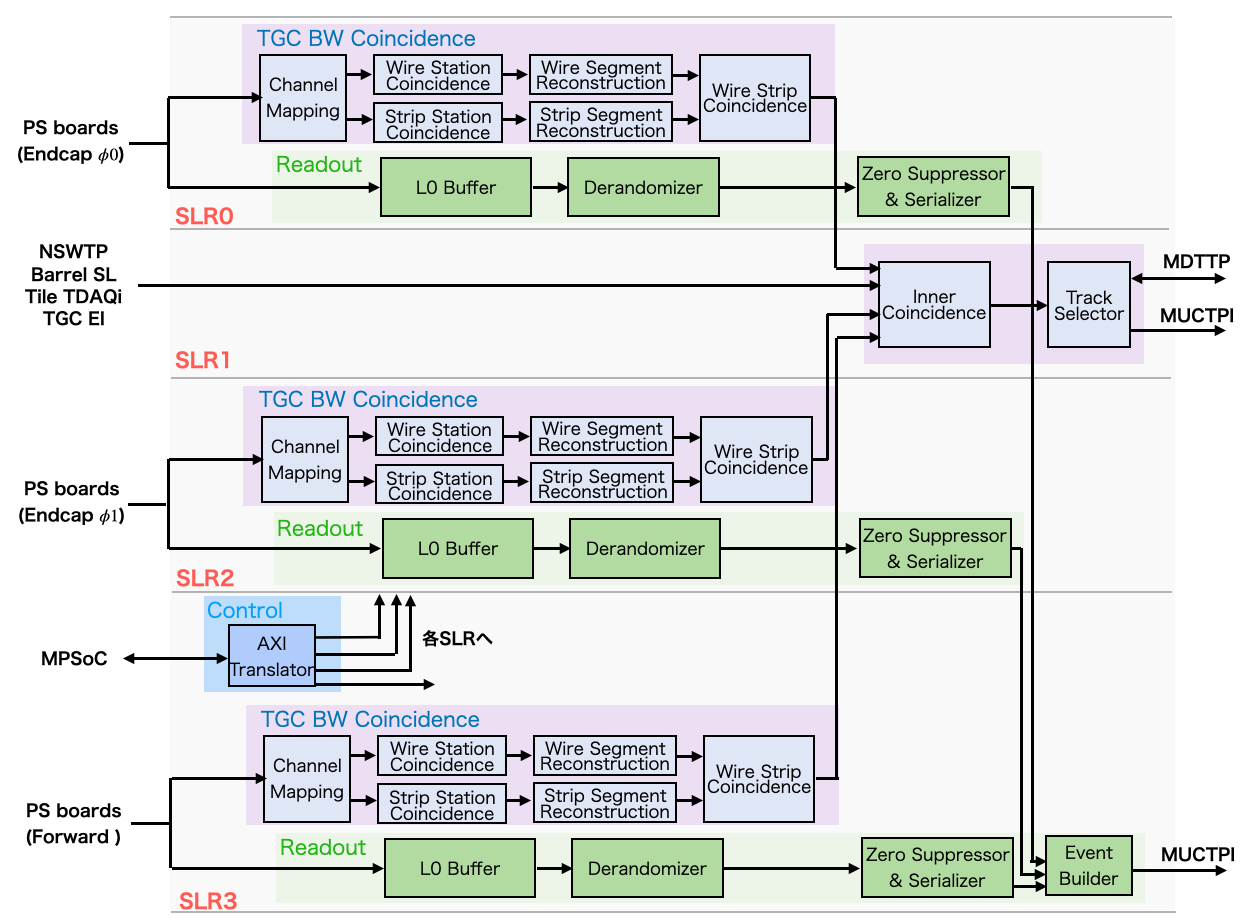
\includegraphics[width=16cm]{fig/Intro/SL_floor.png}
\caption[SL FPGA全体像]{SL FPGAの全体像}
\label{SL_floor}
\end{figure}



    \subsubsection*{Zynq MPSoC}
Zynq MPSoCはSL FPGAおよびPS boardのコントロールマスターとして動作する。加えてATLASのTDAQシステムやDetector Control System (DCS)とのインターフェイスとしての役割も果たす。
Zynq MPSoCもPSとPLから構成されるシリコンデバイスである。PSにはプロセッサやメモリが搭載されていて、SLでは標準的なOSであるCentOS7を起動する。ユーザーはネットワークを通じてSLにアクセスし、PSとPL間の通信を介してPLを操作することができる。SLのMPSoCはEnclustra社が開発しているMercury XC5メザニンカードに搭載されている。このメザニンにはSL FPGと高速通信を行うためのIOが搭載されており、チップ間通信を介してMPSoCのPSからSL FPGAを操作することができる。
Mercury XU5には他にも、DDR4 SDRAMやeMMC、Gigabit Ethernet PHY、USB PHY、QSPI フラッシュメモリなどが搭載されている。市販のメザニンを活用することで、SLボードの開発コストを下げることに加え、メンテナンスを容易にすることができる。Mercury XU5メザニンカードの構造と、SLボード上における接続関係を図\ref{SL_mezanin}に示す。

\begin{figure} 
\centering
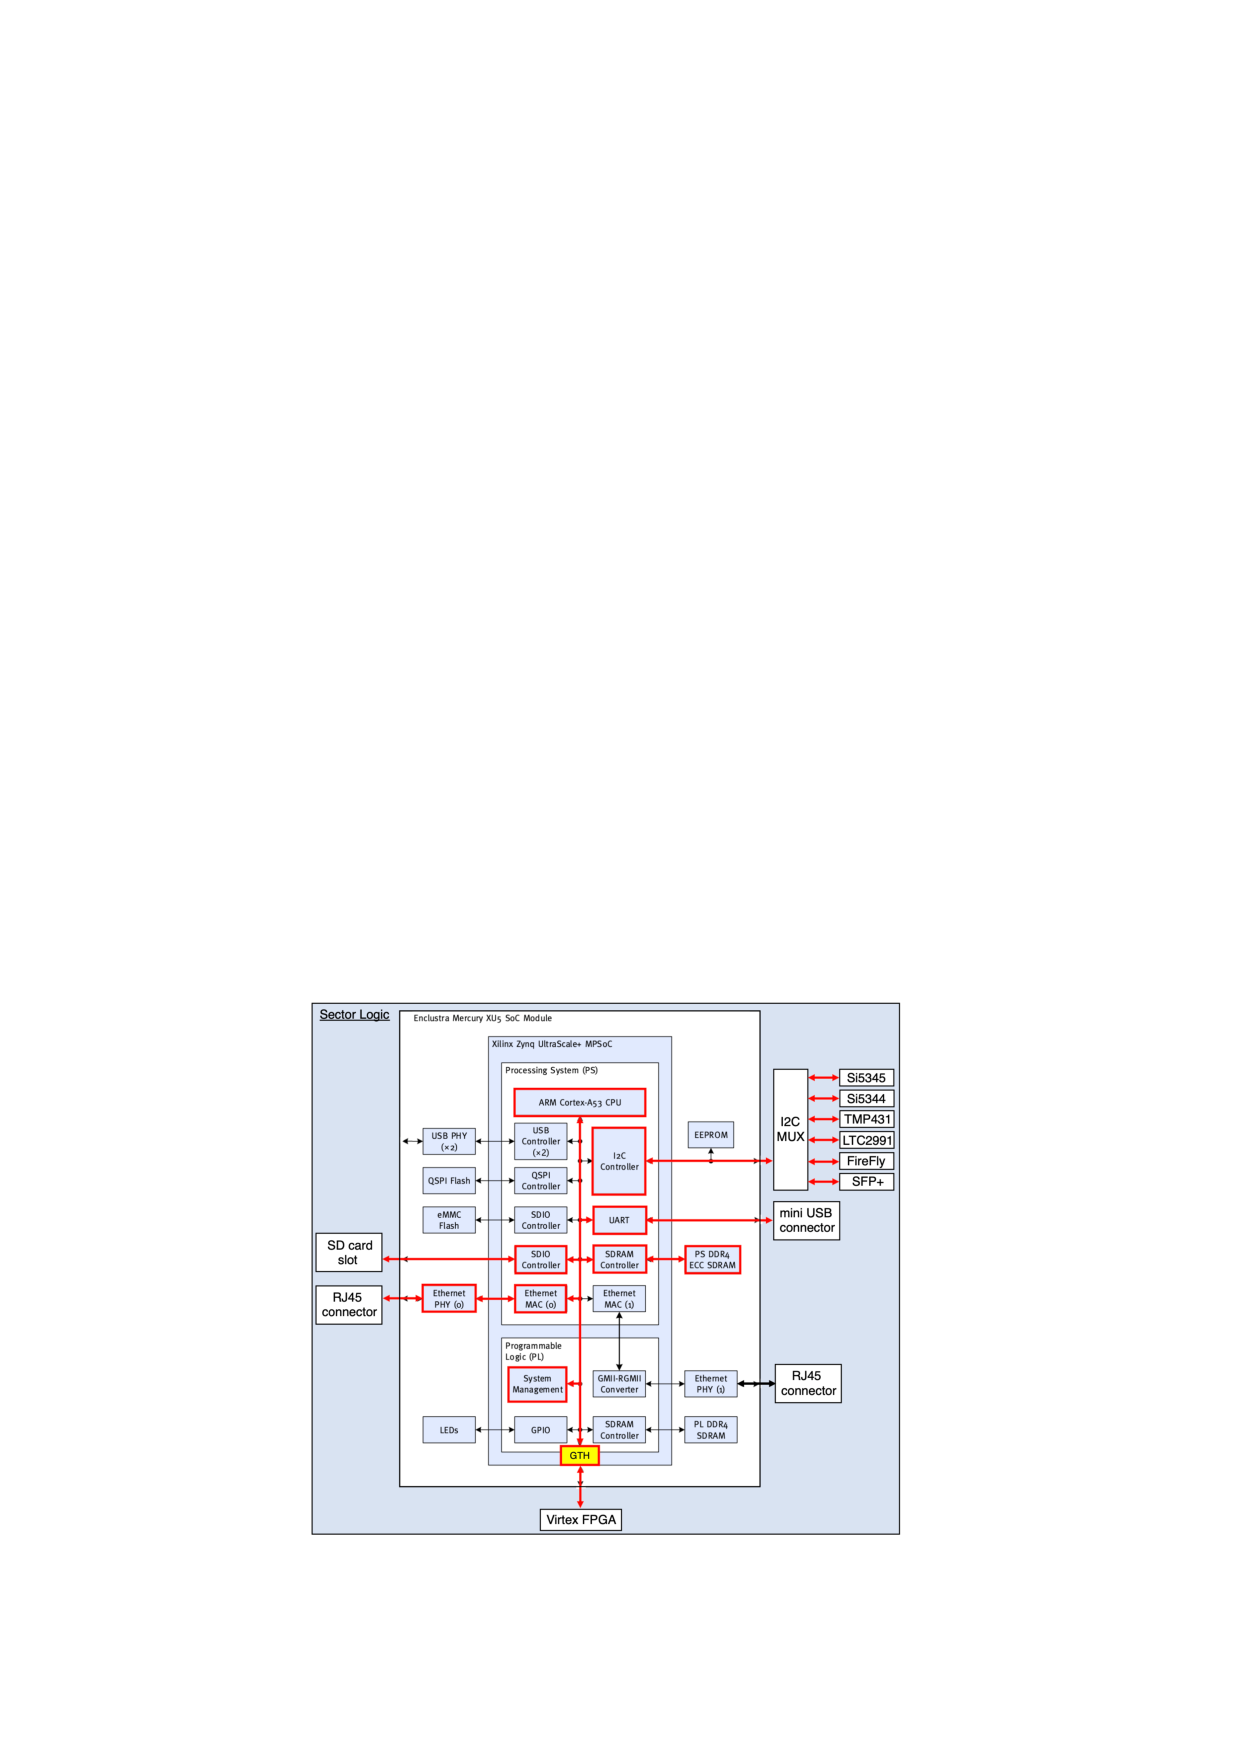
\includegraphics[width=16cm]{fig/Intro/SL_mezanin.pdf}
\caption[Mercury XU5 メザニンカードの構造とSLボード上における接続関係]{Mercury XU5 メザニンカードの構造とSLボード上における接続関係\cite{mt_mishima}}
\label{SL_mezanin}
\end{figure}